\documentclass[11pt]{article}

% ==============================================================================
%  Supporting Information (SI)
%  Manuscript: PhysiChem-GTX: A Physics Informed Dual Stream Framework
%              for Predicting Micropollutant Rejection in NF/RO Membranes
%  Target Outlets: ACS ES&T Engineering / Water Research / J. Membrane Science
% ==============================================================================

\usepackage[utf8]{inputenc}
\usepackage[T1]{fontenc}
\usepackage[margin=2.5cm]{geometry}
\usepackage{setspace}
\setstretch{1.15}
\usepackage{times}
\usepackage{amsmath,amssymb,amsfonts}
\usepackage{cite}
\usepackage{graphicx}
\usepackage{booktabs}
\usepackage{array}
\usepackage{multirow}
\usepackage{longtable}
\usepackage{tabularx}
\usepackage{float}
\usepackage{placeins}
\usepackage{caption}
\usepackage[hidelinks,colorlinks=true,citecolor=blue,linkcolor=blue,urlcolor=blue]{hyperref}
\usepackage{authblk}
\usepackage{titlesec}
\usepackage{enumitem}
\usepackage{xcolor}
\usepackage{siunitx}
\usepackage{fancyhdr}
\usepackage{listings}
\usepackage{algorithm}
\usepackage{algpseudocode}

\graphicspath{{./}{./figures/}{figures/}{../results/paper_figures/}{results/paper_figures/}}

% Supplementary Prefix Setup (S1, S2, Table S1, Figure S1, Eq. S1)
\renewcommand{\thesection}{S\arabic{section}}
\renewcommand{\thesubsection}{S\arabic{section}.\arabic{subsection}}
\renewcommand{\thesubsubsection}{S\arabic{section}.\arabic{subsection}.\arabic{subsubsection}}
\renewcommand{\thetable}{S\arabic{table}}
\renewcommand{\thefigure}{S\arabic{figure}}
\renewcommand{\theequation}{S\arabic{equation}}

\titleformat{\section}{\normalfont\large}{\thesection.}{0.6em}{}
\titleformat{\subsection}{\normalfont\normalsize}{\thesubsection}{0.6em}{}
\titleformat{\subsubsection}{\normalfont\normalsize\itshape}{\thesubsubsection}{0.6em}{}

\pagestyle{fancy}
\fancyhf{}
\fancyfoot[C]{\footnotesize Page S\thepage}
\renewcommand{\headrulewidth}{0pt}
\renewcommand{\footrulewidth}{0pt}

\captionsetup{font=small,justification=justified}
\newcommand{\rsq}{R^{2}}

\begin{document}

% ==============================================================================
% TITLE & AUTHOR METADATA
% ==============================================================================
\begin{center}
    {\Large Supporting Information for:}\\[0.4cm]
    {\LARGE PhysiChem-GTX: A Physics Informed Dual Stream Framework for Predicting Micropollutant Rejection in NF/RO Membranes}\\[0.8cm]

    {\large Raghav Gupta, Atulya Ishan, Krutarth Rupala, Aryan Tripathi}\\[0.3cm]
    {\normalsize \textit{Department of Data Science and Engineering, Manipal Institute of Technology,}}\\
    {\normalsize \textit{Manipal Academy of Higher Education, Manipal, Karnataka 576104, India}}\\[0.6cm]
\end{center}

\vspace{0.6cm}

% ==============================================================================
% TABLE OF CONTENTS / OUTLINE OF SUPPORTING INFORMATION
% ==============================================================================
\noindent{\large Table of Contents / Supplementary Outline}
\begin{itemize}[leftmargin=1.5cm, label=$\blacktriangleright$]
    \item Section S1: Separation Science Theory \& Physical Feature Derivations
    \begin{itemize}[label=$\circ$]
        \item S1.1: Extended Nernst-Planck Continuum Mass Transfer \& Interfacial Partitioning
        \item S1.2: Rigorous Derivations of the Five Physics Descriptors (Eq.~1 to Eq.~5 in Main Paper)
        \begin{itemize}[label=--]
            \item S1.2.1: Steric Sieve Ratio ($\lambda$, Eq.~1)
            \item S1.2.2: Ferry-Renkin Parabolic Convective Partition Factor ($\Phi$, Eq.~2)
            \item S1.2.3: Intrinsic Hydraulic Permeability ($L_p$, Eq.~3)
            \item S1.2.4: Electrostatic Donnan Interaction Index ($\Psi$, Eq.~4)
            \item S1.2.5: Thermodynamic Interfacial Adsorption Affinity ($H$, Eq.~5)
        \end{itemize}
        \item S1.3: Hydrodynamic Wall Drag Coefficients ($K_c, K_d$) in Laminar Stokes Flow
        \item S1.4: Dielectric and Solvation Energy Exclusion (Born \& Onsager Formulations)
    \end{itemize}
    \item Section S2: Benchmark Dataset Description \& Chemical Diversity
    \begin{itemize}[label=$\circ$]
        \item S2.1: Data Acquisition Protocol and Literature Harmonization
        \item S2.2: Description of the 19 Raw Experimental Descriptors (Table S1)
        \item S2.3: Specification Atlas of Commercial NF/RO Membranes (Table S2)
        \item S2.4: Comprehensive Catalog of the 169 Micropollutants (Table S3)
        \item S2.5: Cross-Feature Multicollinearity \& Correlation Heatmap (Figure S1)
    \end{itemize}
    \item Section S3: Complete Architecture Formulations \& Dual-Stream Derivations
    \begin{itemize}[label=$\circ$]
        \item S3.1: Attributed Molecular Graph Representation and 3D Conformer Featurization
        \item S3.2: Edge-Augmented Graph Attention Network (GATv2) Node Update (Eq.~6 in Main Paper)
        \item S3.3: Dynamic Bond-Aware Attention Softmax Mechanism (Eq.~7 in Main Paper)
        \item S3.4: Tri-Moment Multi-Scale Statistical Readout Pooling Layer (Eq.~8 in Main Paper)
        \item S3.5: Cross-Modal Tabular-Graph Conditioning Attention
        \item S3.6: Structural Layer Dimensions of PhysiChem-GT (Table S4)
        \item S3.7: Total Composite Huber Loss Function (Eq.~9 in Main Paper)
        \item S3.8: One-Sided Quadratic Steric Barrier Penalty (Eq.~10 in Main Paper)
        \item S3.9: Monotonic Gradient-Boosted Trees (PhysiChem-XGB) \& Split Constraints (Eq.~11 in Main Paper, Table S5)
        \item S3.10: Calibrated Hydrodynamic Gating Function (Eq.~12 in Main Paper), Dual-Stream Mixture (Eq.~13 in Main Paper), and Steric Monotonicity Proof (Theorem S1)
        \item S3.11: Dual-Stream Epistemic Uncertainty Propagation Formulation (Eq.~14 in Main Paper)
    \end{itemize}
    \item Section S4: Extended Experimental Benchmarks \& Uncertainty Quantification
    \begin{itemize}[label=$\circ$]
        \item S4.1: Full Benchmark Comparison Across 10 Baseline Models (Table S6)
        \item S4.2: Residual Error Distribution \& Outlier Physicochemical Case Studies (Figure S2)
        \item S4.3: Epistemic Uncertainty Estimation \& Calibration Reliability Diagrams (Figure S3)
    \end{itemize}
    \item Section S5: Complete End-to-End Computational Walkthrough: Step-by-Step Rejection Calculation
    \begin{itemize}[label=$\circ$]
        \item S5.1: Representative Case Definition (Ibuprofen on Commercial FilmTec NF90)
        \item S5.2: Stage 1: Explicit Physics-Informed Feature Engineering (From Scratch)
        \item S5.3: Stage 2: Deep Neural Stream (PhysiChem-GT) Graph Processing
        \item S5.4: Stage 3: Monotonic Physics Booster (PhysiChem-XGB) Tree Evaluation
        \item S5.5: Stage 4: Hydrodynamic Gating, Blending, and Hard-Constraint Enforcement
        \item S5.6: Comprehensive Numerical Trace \& Ground-Truth Validation
    \end{itemize}
    \item Supplementary References
\end{itemize}

\newpage

% ==============================================================================
% SECTION S1: SEPARATION SCIENCE THEORY & PHYSICAL FEATURE DERIVATIONS
% ==============================================================================
\section{Separation Science Theory \& Physical Feature Derivations}
\label{sec:theory}

\subsection{Extended Nernst-Planck Continuum Mass Transfer \& Interfacial Partitioning}
\label{sec:dspm}
Solute transport through thin-film composite (TFC) nanofiltration and reverse osmosis active polyamide separation layers ($\Delta x$) is fundamentally governed by the one-dimensional Extended Nernst-Planck equation. For any dissolved micropollutant or ionic solute $i$, the axial solute flux $J_i$ combines hindered diffusion, convective solvent drag, and electromigrative drift:
\begin{equation}
J_i = -K_{i,d} D_{i,\infty} \frac{dc_i}{dx} - \frac{z_i c_i K_{i,d} D_{i,\infty} F}{RT} \frac{d\psi}{dx} + K_{i,c} c_i V
\label{eq:s_enp}
\end{equation}
where:
\begin{itemize}[leftmargin=1.0cm]
    \item $c_i(x)$ is the local intra-pore solute concentration at axial depth $x \in [0, \Delta x]$,
    \item $D_{i,\infty} = \frac{k_B T}{6 \pi \eta r_s}$ is the infinite-dilution Stokes-Einstein bulk diffusivity in water with dynamic viscosity $\eta$,
    \item $z_i$ is the solute formal net valence,
    \item $F$ is Faraday's constant ($96{,}485\text{ C}\cdot\text{mol}^{-1}$),
    \item $\psi(x)$ is the local electrostatic potential within the pore channel,
    \item $V = J_w / \varepsilon$ is the convective solvent pore velocity through porosity $\varepsilon$,
    \item $K_{i,d}(\lambda)$ and $K_{i,c}(\lambda)$ represent the hydrodynamic diffusive and convective hindrance factors.
\end{itemize}

At the solution-membrane interfaces (feed entrance $x = 0$ and permeate exit $x = \Delta x$), thermodynamic phase equilibrium establishes the interface partitioning coefficient $\phi_i$:
\begin{equation}
\frac{c_i(0^+)}{c_i(0^-)} = \phi_i = \Phi_i \cdot \exp\left(-\frac{z_i F \Delta \psi_D}{RT}\right) \cdot \exp\left(-\frac{\Delta W_i}{k_B T}\right)
\label{eq:s_partitioning}
\end{equation}
where $\Phi_i$ is the steric exclusion coefficient, $\Delta \psi_D$ is the interfacial Donnan electric potential difference, and $\Delta W_i$ is the dielectric solvation self-energy exclusion barrier.

% ------------------------------------------------------------------------------
\subsection{Rigorous Derivations of the Five Physics Descriptors (Eq.~1 to Eq.~5)}
\label{sec:physics_descriptors_derivation}

In Section~2.2 of the main manuscript, five mechanistically grounded physical transport descriptors are embedded into the feature representation to constrain model predictions within thermodynamic boundaries. Below, we provide the complete mathematical derivations for each descriptor:

\subsubsection{1. Steric Sieve Ratio ($\lambda$, Eq.~1 in Main Paper)}
\begin{equation}
\lambda = \frac{r_{\mathrm{solute}}}{r_{\mathrm{pore}}}
\label{eq:s_lambda}
\end{equation}
\noindent\textit{Detailed Derivation:} Consider a rigid spherical molecule approaching a cylindrical membrane pore of uniform hydraulic radius $r_{\mathrm{pore}}$. The solute's hydrodynamic boundary is defined by its Stokes-Einstein radius $r_{\mathrm{solute}}$, derived from infinite-dilution diffusivity $D_\infty$:
\begin{equation}
r_{\mathrm{solute}} = \frac{k_B T}{6 \pi \eta D_\infty}
\label{eq:s_stokes_einstein}
\end{equation}
Because the hard atomic core of the solute cannot penetrate the electronic electron clouds of the pore wall, the center of mass of the solute is strictly restricted to radial coordinates $r \le (r_{\mathrm{pore}} - r_{\mathrm{solute}})$. The ratio $\lambda$ represents the dimensionless steric confinement parameter:
\begin{itemize}[leftmargin=1.0cm]
    \item When $\lambda < 1.0$, a non-zero radial channel core ($0 \le r \le r_{\mathrm{pore}}(1 - \lambda)$) is accessible for convective and diffusive entry.
    \item When $\lambda \ge 1.0$, $r_{\mathrm{solute}} \ge r_{\mathrm{pore}}$. Zero center-of-mass positions are kinematically accessible, establishing the physical threshold of total geometric sieving.
\end{itemize}

\subsubsection{2. Ferry-Renkin Parabolic Convective Partition Factor ($\Phi$, Eq.~2 in Main Paper)}
\begin{equation}
\Phi(\lambda) = (1-\lambda)^2 \left[2 - (1-\lambda)^2\right], \quad \lambda < 1.0
\label{eq:s_ferry_renkin}
\end{equation}
\noindent\textit{Detailed Derivation:} In fully developed laminar Stokes flow through a cylindrical capillary of radius $r_p$, the fluid velocity profile $u(r)$ as a function of radial position $r \in [0, r_p]$ is governed by the Hagen-Poiseuille equation:
\begin{equation}
u(r) = 2 \bar{u} \left(1 - \frac{r^2}{r_p^2}\right)
\label{eq:s_poiseuille}
\end{equation}
where $\bar{u}$ is the cross-sectional mean fluid velocity. The total convective volumetric fluid flux $Q_{\mathrm{total}}$ across the entire pore lumen is:
\begin{equation}
Q_{\mathrm{total}} = \int_0^{r_p} u(r) \cdot 2\pi r \, dr = 2\bar{u} \cdot 2\pi \int_0^{r_p} \left(r - \frac{r^3}{r_p^2}\right) dr = 4\pi\bar{u} \left[ \frac{r_p^2}{2} - \frac{r_p^4}{4r_p^2} \right] = \pi r_p^2 \bar{u}
\label{eq:s_q_total}
\end{equation}
A spherical solute of radius $r_s = \lambda r_p$ can only be transported through the accessible center-of-mass cross-section $0 \le r \le (r_p - r_s) = r_p(1 - \lambda)$. The convective solute flux $Q_{\mathrm{accessible}}$ carried through this accessible core is:
\begin{equation}
Q_{\mathrm{accessible}} = \int_0^{r_p(1-\lambda)} u(r) \cdot 2\pi r \, dr = 4\pi\bar{u} \int_0^{r_p(1-\lambda)} \left( r - \frac{r^3}{r_p^2} \right) dr
\label{eq:s_q_accessible}
\end{equation}
Evaluating the definite integral:
\begin{align}
Q_{\mathrm{accessible}} &= 4\pi\bar{u} \left[ \frac{r^2}{2} - \frac{r^4}{4r_p^2} \right]_0^{r_p(1-\lambda)} \nonumber \\
&= 4\pi\bar{u} \left[ \frac{r_p^2(1-\lambda)^2}{2} - \frac{r_p^4(1-\lambda)^4}{4r_p^2} \right] \nonumber \\
&= 4\pi\bar{u} r_p^2 (1-\lambda)^2 \left[ \frac{1}{2} - \frac{(1-\lambda)^2}{4} \right] \nonumber \\
&= \pi r_p^2 \bar{u} (1-\lambda)^2 \left[ 2 - (1-\lambda)^2 \right]
\label{eq:s_integral_eval}
\end{align}
The convective partitioning factor $\Phi(\lambda)$ is the ratio of accessible convective flux to total fluid flux:
\begin{equation}
\Phi(\lambda) = \frac{Q_{\mathrm{accessible}}}{Q_{\mathrm{total}}} = \frac{\pi r_p^2 \bar{u} (1-\lambda)^2 \left[ 2 - (1-\lambda)^2 \right]}{\pi r_p^2 \bar{u}} = (1-\lambda)^2 \left[ 2 - (1-\lambda)^2 \right]
\label{eq:s_phi_final}
\end{equation}
Equation~(\ref{eq:s_ferry_renkin}) decomposes into two distinct physical factors:
\begin{enumerate}[leftmargin=1.0cm]
    \item $(1 - \lambda)^2 = \frac{\pi r_p^2(1-\lambda)^2}{\pi r_p^2}$: The purely geometric cross-sectional area ratio accessible to the solute center of mass.
    \item $\left[2 - (1 - \lambda)^2\right] = 1 + 2\lambda - \lambda^2 \ge 1$: The parabolic velocity weighting term, accounting for the fact that fluid streamlines travel fastest near the centerline where the solute resides.
\end{enumerate}
The baseline theoretical steric rejection prior is $R_{\mathrm{theory}} = (1.0 - \Phi(\lambda)) \times 100\%$.

\subsubsection{3. Intrinsic Hydraulic Permeability ($L_p$, Eq.~3 in Main Paper)}
\begin{equation}
L_p = \frac{J_w}{\Delta P} \quad \left[\mathrm{L\,m^{-2}\,h^{-1}\,bar^{-1}}\right]
\label{eq:s_lp}
\end{equation}
\noindent\textit{Detailed Derivation:} According to Darcy's law for flow through porous media, the superficial fluid flux $J_w$ driven across a selective membrane layer of thickness $\Delta x$ and tortuosity $\tau_p$ is:
\begin{equation}
J_w = \frac{K_m}{\eta \Delta x} \Delta P
\label{eq:s_darcy_law}
\end{equation}
where $K_m$ is the intrinsic permeability of the porous matrix. In the pore bundle model (Hagen-Poiseuille representation with porosity $\varepsilon$ and mean pore radius $r_p$), the permeability coefficient is $K_m = \frac{\varepsilon r_p^2}{8\tau_p}$. Substituting this gives:
\begin{equation}
J_w = \left( \frac{\varepsilon r_p^2}{8\eta \tau_p \Delta x} \right) \Delta P
\label{eq:s_darcy_hp}
\end{equation}
Dividing $J_w$ by the net applied transmembrane driving pressure $\Delta P$ yields the intrinsic hydraulic permeability $L_p = \frac{\varepsilon r_p^2}{8\eta \tau_p \Delta x}$. This parameter isolates the physical compaction resistance and morphological thickness-to-porosity ratio of the selective polyamide layer from operational pressure fluctuations.

\subsubsection{4. Electrostatic Donnan Interaction Index ($\Psi$, Eq.~4 in Main Paper)}
\begin{equation}
\Psi = \frac{z \cdot \zeta}{\mathrm{pH}} \quad [\mathrm{mV}]
\label{eq:s_psi}
\end{equation}
\noindent\textit{Detailed Derivation:} In Gouy-Chapman electrical double-layer theory, the fixed volumetric charge density of a charged membrane surface creates an interfacial electrostatic potential $\psi_0$, which is directly monitored experimentally via the streaming potential (zeta potential, $\zeta$). The electrostatic free energy of bringing a solute with formal ionic valence $z$ from bulk solution to the membrane interface is:
\begin{equation}
\Delta G_{\mathrm{elec}} = z F \Delta \psi_D \propto z \cdot \zeta
\label{eq:s_elec_energy}
\end{equation}
Because the deprotonation of membrane carboxylic functional groups ($-\mathrm{COOH} \rightleftharpoons -\mathrm{COO}^- + \mathrm{H}^+$) and the protonation of unreacted amine cross-links ($-\mathrm{NH}_2 + \mathrm{H}^+ \rightleftharpoons -\mathrm{NH}_3^+$) follow Henderson-Hasselbalch equilibria governed by hydrogen ion activity, normalizing $z \cdot \zeta$ by feed $\mathrm{pH}$ yields the electrostatic interaction index $\Psi$. When $z$ and $\zeta$ have the same sign (e.g., anionic solute $z = -1$ encountering a negatively charged membrane $\zeta = -30\text{ mV}$ at neutral $\mathrm{pH}$), $\Psi > 0$, driving strong Donnan electrostatic repulsion and boosting rejection.

\subsubsection{5. Thermodynamic Interfacial Adsorption Affinity ($H$, Eq.~5 in Main Paper)}
\begin{equation}
H = \log D \cdot \cos(\theta)
\label{eq:s_h_affinity}
\end{equation}
\noindent\textit{Detailed Derivation:} The thermodynamic work of adhesion $W_{SL}$ between a liquid solution ($L$) and a solid polyamide membrane surface ($S$) in vapor ($V$) is formulated by the Young-Dupr\'e equation:
\begin{equation}
W_{SL} = \gamma_{LV} (1 + \cos\theta)
\label{eq:s_young_dupre}
\end{equation}
where $\gamma_{LV}$ is the liquid surface tension and $\theta$ is the sessile drop contact angle. As the membrane surface becomes more hydrophobic ($\theta \to 90^\circ$, $\cos\theta \to 0$), water molecules are less strongly bound to the polyamide matrix, lowering the dehydration energy barrier for organic solutes. The distribution coefficient $\log D$ measures the effective lipophilicity of the solute at operational feed pH:
\begin{equation}
\log D = \log K_{ow} - \log\left( 1 + 10^{\mathrm{pH} - \mathrm{p}K_a} \right) \quad \text{(for monoprotic acids)}
\label{eq:s_logd_def}
\end{equation}
Coupling $\log D$ with $\cos\theta$ parameterizes the thermodynamic free energy of organic solute hydrophobic partitioning into the membrane polymer matrix, separating matrix sorption from convective drag.

% ------------------------------------------------------------------------------
\subsection{Hydrodynamic Wall Drag Coefficients ($K_c, K_d$) in Laminar Stokes Flow}
\label{sec:ferry_renkin_drag}
Beyond the cross-sectional partition factor $\Phi(\lambda)$, intra-pore solute motion is hindered by frictional shear stresses against the pore walls. The convective drag coefficient $K_c(\lambda)$ and diffusive hindrance factor $K_d(\lambda)$ in Equation~(\ref{eq:s_enp}) are expressed using standard polynomial expansions for centerline laminar Stokes flow:
\begin{align}
K_c(\lambda) &= (2 - \Phi) \left[ 1 + 0.054 \lambda - 0.988 \lambda^2 + 0.441 \lambda^3 \right] \label{eq:s_kc} \\
K_d(\lambda) &= 1 - 2.104 \lambda + 2.089 \lambda^2 - 0.948 \lambda^3 \label{eq:s_kd}
\end{align}
Equations~(\ref{eq:s_kc}) and (\ref{eq:s_kd}) ensure that as $\lambda \to 1.0$, $K_d(\lambda) \to 0$ (molecular diffusion across the pore is completely arrested) and $K_c(\lambda) \to 0$, enforcing total hydrodynamic retention.

% ------------------------------------------------------------------------------
\subsection{Dielectric and Solvation Energy Exclusion (Born \& Onsager Formulations)}
\label{sec:dielectric_exclusion}
Within sub-nanometer membrane pores ($r_p \le 0.50\text{ nm}$), dipolar dielectric relaxation of confined water molecules is restricted. The local pore dielectric permittivity drops from bulk water ($\varepsilon_b \approx 80.4$) to confined pore water ($\varepsilon_p \approx 30 - 45$). The resulting Born solvation self-energy barrier $\Delta W_i$ experienced by an ion or charged solute of cavity radius $r_i$ is:
\begin{equation}
\Delta W_i = \frac{z_i^2 e^2}{8 \pi \varepsilon_0 r_i} \left( \frac{1}{\varepsilon_p} - \frac{1}{\varepsilon_b} \right)
\label{eq:s_born_energy}
\end{equation}
For neutral organic compounds with an electric dipole moment $\mu_D$, the reaction-field polarization produces an analogous quadratic barrier:
\begin{equation}
\Delta W_{\text{dipole}} = \frac{\mu_D^2}{4 \pi \varepsilon_0 r_s^3} \left[ \frac{\varepsilon_b - 1}{2\varepsilon_b + 1} - \frac{\varepsilon_p - 1}{2\varepsilon_p + 1} \right]
\label{eq:s_onsager_energy}
\end{equation}
This dielectric exclusion mechanism explains why even neutral solutes with significant polar surface area (TPSA) achieve high experimental rejections ($>85\%$) in tight NF membranes despite having $\lambda < 1.0$.

\newpage

% ==============================================================================
% SECTION S2: BENCHMARK DATASET DESCRIPTION & CHEMICAL DIVERSITY
% ==============================================================================
\section{Benchmark Dataset Description and Chemical Diversity}
\label{sec:dataset}

\subsection{Data Acquisition Protocol and Literature Harmonization}
The MemTrOC benchmark corpus was curated from $16$ authoritative experimental literature sources spanning global water research institutions. The dataset comprises $N = 1{,}618$ distinct filtration runs operating under strict bench-scale cross-flow filtration protocols:
\begin{itemize}[leftmargin=0.8cm, topsep=2pt, itemsep=1pt, parsep=0pt]
    \item Equilibrium Criteria: Rejection measurements were recorded only after steady-state permeate flux was achieved ($>4\text{ h}$ pre-compaction, $12 - 48\text{ h}$ total filtration duration).
    \item Feed Water Matrices: Real surface waters, secondary wastewater effluents, and synthetic electrolyte matrices ($0.001 - 0.1\text{ M}$ NaCl/$\text{CaCl}_2$, $\text{pH } 3.0 - 10.5$).
    \item Chemical Harmonization: All micropollutant chemical names were reconciled with PubChem CIDs and assigned canonical stereochemically unraveled SMILES strings using RDKit Release 2023.09.
\end{itemize}

\subsection{Comprehensive Description of the 19 Raw Experimental Descriptors}
The 19 experimental raw features span operational filtration conditions, membrane physicochemical specifications, and solute quantum/topological properties as detailed in Table~\ref{tab:s1_descriptors}.

\begin{table}[H]
\centering
\footnotesize
\renewcommand{\arraystretch}{0.84}
\setlength{\tabcolsep}{3.0pt}
\caption{Comprehensive specification of the 19 raw input features in the MemTrOC benchmark corpus. Features span operating conditions, membrane physicochemical properties, and solute quantum/topological descriptors.}
\label{tab:s1_descriptors}
\begin{tabularx}{\textwidth}{c l c c >{\raggedright\arraybackslash}X}
\toprule
Index & Descriptor Name & Units & Observed Range & Separation Mechanism / Role \\
\midrule
0  & Pore radius ($r_p$)         & \si{\nano\meter} & 0.25 -- 0.70 & Steric sieving and hydrodynamic drag \\
1  & Pure water flux ($J_w$)     & \si{\liter\per\meter\squared\per\hour} & 10.0 -- 180.0 & Convective solvent throughput \\
2  & Operating pressure ($\Delta P$) & \si{\bar} & 2.0 -- 20.0 & Transmembrane convective driving force \\
3  & Membrane zeta potential ($\zeta_m$) & \si{\milli\volt} & $-45.0$ -- $+10.0$ & Donnan electrostatic repulsion/attraction \\
4  & Feed pH                     & -- & 3.0 -- 10.5 & Governs ionization states ($\text{p}K_a$) \\
5  & Contact angle ($\theta$)    & degrees ($^\circ$) & 20.0 -- 75.0 & Membrane surface hydrophobicity \\
6  & Temperature ($T$)           & \si{\celsius} & 15.0 -- 35.0 & Water viscosity and solute diffusivity \\
7  & Feed solute concentration   & \si{\micro\mol\per\liter} & 0.1 -- 50.0 & Concentration polarization potential \\
8  & Background ionic strength   & \si{\mol\per\liter} & 0.001 -- 0.100 & Electrical double layer Debye screening \\
9  & Cross-flow velocity ($v$)   & \si{\meter\per\second} & 0.1 -- 2.5 & Boundary layer shear and mass transfer \\
10 & Molecular Stokes radius ($r_s$) & \si{\nano\meter} & 0.25 -- 0.85 & Hydrodynamic molecular size \\
11 & Molecular weight (MW)       & \si{\gram\per\mol} & 100.0 -- 800.0 & Molecular mass \\
12 & Net molecular charge ($z_s$)& integer & $-2, -1, 0, +1$ & Formal ionic state at operational pH \\
13 & $\log D$                    & log & $-3.0$ -- $+5.0$ & pH-dependent lipophilicity/hydrophobicity \\
14 & Molecular polarizability    & \si{\angstrom\cubed} & 10.0 -- 60.0 & Electronic dispersion and dipole forces \\
15 & Polar surface area (TPSA)   & \si{\angstrom\squared} & 10.0 -- 180.0 & Hydrogen-bonding and solvation capacity \\
16 & Hydrogen bond donors        & count & 0 -- 6 & Specific hydrogen-bonding with membrane matrix \\
17 & Hydrogen bond acceptors     & count & 1 -- 12 & Lewis base hydration sites \\
18 & Rotatable bonds             & count & 0 -- 15 & Conformational flexibility in pore confinement \\
\bottomrule
\end{tabularx}
\end{table}

\newpage

\subsection{Specification Atlas of Commercial NF/RO Membranes}
\label{sec:membrane_atlas}
The experimental observations in the MemTrOC corpus are derived predominantly ($>85\%$) from 16 commercial thin-film composite (TFC) nanofiltration and reverse osmosis membranes. Table~\ref{tab:s2_membranes} catalogs their manufacturer, polymer classification, molecular weight cut-off (MWCO), pore radius ($r_p$), isoelectric point (IEP), and water contact angle.

\begin{table}[H]
\centering
\small
\setlength{\tabcolsep}{3.5pt}
\renewcommand{\arraystretch}{0.92}
\caption{Morphological, surface charge, and transport properties of the dominant commercial NF/RO membranes in the MemTrOC corpus (accounting for $>85\%$ of experimental observations).}
\label{tab:s2_membranes}
\begin{tabularx}{\textwidth}{>{\raggedright\arraybackslash}p{2.6cm} >{\raggedright\arraybackslash}p{2.8cm} >{\raggedright\arraybackslash}X c c c c}
\toprule
Membrane & Manufacturer & Polymer Class & \begin{tabular}{@{}c@{}}MWCO\\(Da)\end{tabular} & \begin{tabular}{@{}c@{}}$r_p$\\(nm)\end{tabular} & \begin{tabular}{@{}c@{}}IEP\\(pH)\end{tabular} & \begin{tabular}{@{}c@{}}Contact\\Angle ($^\circ$)\end{tabular} \\
\midrule
FilmTec NF90     & DuPont / FilmTec           & Fully aromatic polyamide    & 100 -- 200 & 0.34 & 4.0 & 54 \\
FilmTec NF270    & DuPont / FilmTec           & Polypiperazine amide        & 200 -- 400 & 0.42 & 3.5 & 30 \\
FilmTec XLE      & DuPont / FilmTec           & Fully aromatic polyamide    & $<100$     & 0.30 & 4.0 & 58 \\
Desal-HL (De-HL) & Suez / GE Osmonics         & Polypiperazine amide        & 150 -- 300 & 0.40 & 3.8 & 40 \\
NF200            & Woongjin Chemical          & Polypiperazine amide        & 150 -- 300 & 0.38 & 3.9 & 44 \\
Toray UTC-60     & Toray Industries           & Cross-linked polyamide      & 200 -- 350 & 0.37 & 4.5 & 48 \\
Hydranautics ES20& Nitto Denko / Hydranautics & Polyamide                   & 150 -- 250 & 0.36 & 4.2 & 52 \\
TriSep TS80      & Microdyn-Nadir / TriSep    & Polyamide                   & 100 -- 200 & 0.35 & 4.1 & 56 \\
FilmTec BW30     & DuPont / FilmTec           & Fully aromatic polyamide    & $<100$     & 0.28 & 4.2 & 62 \\
Toray UTC-70     & Toray Industries           & Cross-linked polyamide      & 100 -- 200 & 0.32 & 4.3 & 55 \\
FilmTec LE440    & DuPont / FilmTec           & Fully aromatic polyamide    & $<100$     & 0.29 & 4.1 & 60 \\
NTR7450          & Nitto Denko                & Sulfonated polyethersulfone & 600 -- 800 & 0.58 & 2.8 & 38 \\
ESPA1            & Hydranautics               & Cross-linked polyamide      & $<100$     & 0.30 & 4.0 & 57 \\
ESNA             & Hydranautics               & Polyamide                   & 200 -- 300 & 0.39 & 3.6 & 43 \\
Desal-5 DK       & Suez / GE Osmonics         & Polypiperazine amide        & 150 -- 300 & 0.39 & 3.8 & 45 \\
Desal-5 DL       & Suez / GE Osmonics         & Polypiperazine amide        & 150 -- 300 & 0.40 & 4.0 & 42 \\
\bottomrule
\end{tabularx}
\end{table}

\subsection{Comprehensive Catalog of the 169 Micropollutants}
\label{sec:troc_catalog}
The complete library of all 169 micropollutant chemical structures, molecular masses, partition coefficients ($\log K_{ow}$), distribution coefficients at operational pH ($\log D$), and net formal charges ($z_s$) is tabulated in Table~\ref{tab:s3_trocs}, generated directly from the benchmark corpus. Solutes encompass active pharmaceutical ingredients (APIs), endocrine disrupting compounds (EDCs), pesticides, personal care products, and industrial additives spanning diverse functional chemistries.

\clearpage

% Input multi-page longtable (handles flat, folder, and relative structures)
\IfFileExists{table_s3_troc_catalog.tex}{\begin{footnotesize}
\setlength{\tabcolsep}{3.5pt}
\begin{longtable}{>{\raggedright\arraybackslash}p{3.5cm} >{\raggedright\arraybackslash\ttfamily}p{5.8cm} c c c c}
\caption{Comprehensive physicochemical library of all 169 micropollutants compiled in the MemTrOC benchmark corpus. Compounds are listed alphabetically with canonical SMILES representations, molecular weight (MW), octanol-water partition coefficient ($\log K_{ow}$), operational pH distribution coefficient ($\log D$), and formal net charge ($z_s$).}\label{tab:s3_trocs} \\
\toprule
Compound Name & \multicolumn{1}{l}{Canonical SMILES} & \begin{tabular}{@{}c@{}}MW\\(Da)\end{tabular} & $\log K_{ow}$ & $\log D$ & $z_s$ \\
\midrule
\endfirsthead
\multicolumn{6}{c}{{Table \thetable\ continued from previous page}} \\
\toprule
Compound Name & \multicolumn{1}{l}{Canonical SMILES} & \begin{tabular}{@{}c@{}}MW\\(Da)\end{tabular} & $\log K_{ow}$ & $\log D$ & $z_s$ \\
\midrule
\endhead
\midrule
\multicolumn{6}{r}{{\textit{Continued on next page...}}} \\
\bottomrule
\endfoot
\bottomrule
\endlastfoot
1,2-ethanediol & O\allowbreak C\allowbreak C\allowbreak O & 62.1 & -1.36 & -1.36 & 0 \\
1,3-Propandiol & O\allowbreak C\allowbreak C\allowbreak C\allowbreak O & 76.1 & -1.04 & -1.04 & 0 \\
1,4-Butanediol & O\allowbreak C\allowbreak C\allowbreak C\allowbreak C\allowbreak O & 90.1 & -0.83 & -0.83 & 0 \\
1,4-Dioxane & C\allowbreak 1\allowbreak C\allowbreak O\allowbreak C\allowbreak C\allowbreak O\allowbreak 1 & 88.1 & -0.27 & -0.27 & 0 \\
1,5-naphthalenedisulfonic acid & O\allowbreak [\allowbreak S\allowbreak ]\allowbreak (\allowbreak =\allowbreak O\allowbreak )\allowbreak (\allowbreak =\allowbreak O\allowbreak )\allowbreak c\allowbreak 1\allowbreak c\allowbreak c\allowbreak c\allowbreak c\allowbreak 2\allowbreak c\allowbreak 1\allowbreak c\allowbreak c\allowbreak c\allowbreak c\allowbreak 2\allowbreak [\allowbreak S\allowbreak ]\allowbreak (\allowbreak O\allowbreak )\allowbreak (\allowbreak =\allowbreak O\allowbreak )\allowbreak =\allowbreak O & 288.3 & 0.60 & -5.39 & -1 \\
1,5-Pentanediol & O\allowbreak C\allowbreak C\allowbreak C\allowbreak C\allowbreak C\allowbreak O & 104.1 & -0.10 & -0.10 & 0 \\
1-Butanol & C\allowbreak C\allowbreak C\allowbreak C\allowbreak O & 74.1 & 0.88 & 0.88 & 0 \\
17$\alpha$-Estradiol & C\allowbreak [\allowbreak C\allowbreak @\allowbreak ]\allowbreak 1\allowbreak 2\allowbreak C\allowbreak C\allowbreak [\allowbreak C\allowbreak @\allowbreak H\allowbreak ]\allowbreak 3\allowbreak [\allowbreak C\allowbreak @\allowbreak @\allowbreak H\allowbreak ]\allowbreak (\allowbreak C\allowbreak C\allowbreak c\allowbreak 4\allowbreak c\allowbreak c\allowbreak (\allowbreak O\allowbreak )\allowbreak c\allowbreak c\allowbreak c\allowbreak 3\allowbreak 4\allowbreak )\allowbreak [\allowbreak C\allowbreak @\allowbreak @\allowbreak H\allowbreak ]\allowbreak 1\allowbreak C\allowbreak C\allowbreak [\allowbreak C\allowbreak @\allowbreak H\allowbreak ]\allowbreak 2\allowbreak O & 272.4 & 4.01 & 4.01 & 0 \\
17$\alpha$-Ethynilestradiol & C\allowbreak [\allowbreak C\allowbreak @\allowbreak ]\allowbreak 1\allowbreak 2\allowbreak C\allowbreak C\allowbreak [\allowbreak C\allowbreak @\allowbreak H\allowbreak ]\allowbreak 3\allowbreak [\allowbreak C\allowbreak @\allowbreak @\allowbreak H\allowbreak ]\allowbreak (\allowbreak C\allowbreak C\allowbreak c\allowbreak 4\allowbreak c\allowbreak c\allowbreak (\allowbreak O\allowbreak )\allowbreak c\allowbreak c\allowbreak c\allowbreak 3\allowbreak 4\allowbreak )\allowbreak [\allowbreak C\allowbreak @\allowbreak @\allowbreak H\allowbreak ]\allowbreak 1\allowbreak C\allowbreak C\allowbreak [\allowbreak C\allowbreak @\allowbreak @\allowbreak ]\allowbreak 2\allowbreak (\allowbreak O\allowbreak )\allowbreak C\allowbreak \#\allowbreak C & 296.4 & 3.67 & 3.67 & 0 \\
17$\beta$-Estradiol & C\allowbreak [\allowbreak C\allowbreak @\allowbreak ]\allowbreak 1\allowbreak 2\allowbreak C\allowbreak C\allowbreak [\allowbreak C\allowbreak @\allowbreak H\allowbreak ]\allowbreak 3\allowbreak [\allowbreak C\allowbreak @\allowbreak @\allowbreak H\allowbreak ]\allowbreak (\allowbreak C\allowbreak C\allowbreak c\allowbreak 4\allowbreak c\allowbreak c\allowbreak (\allowbreak O\allowbreak )\allowbreak c\allowbreak c\allowbreak c\allowbreak 3\allowbreak 4\allowbreak )\allowbreak [\allowbreak C\allowbreak @\allowbreak @\allowbreak H\allowbreak ]\allowbreak 1\allowbreak C\allowbreak C\allowbreak [\allowbreak C\allowbreak @\allowbreak @\allowbreak H\allowbreak ]\allowbreak 2\allowbreak O & 272.4 & 4.01 & 4.01 & 0 \\
2,3-Dichlorophenol & O\allowbreak c\allowbreak 1\allowbreak c\allowbreak c\allowbreak c\allowbreak c\allowbreak (\allowbreak C\allowbreak l\allowbreak )\allowbreak c\allowbreak 1\allowbreak C\allowbreak l & 163.0 & 2.84 & 2.84 & 0 \\
2,4,5-trichlorophenol & C\allowbreak 1\allowbreak =\allowbreak C\allowbreak (\allowbreak C\allowbreak (\allowbreak =\allowbreak C\allowbreak C\allowbreak (\allowbreak =\allowbreak C\allowbreak 1\allowbreak C\allowbreak l\allowbreak )\allowbreak C\allowbreak l\allowbreak )\allowbreak C\allowbreak l\allowbreak )\allowbreak O & 195.9 & 3.72 & 3.72 & 0 \\
2,4-dichlorophenol & O\allowbreak c\allowbreak 1\allowbreak c\allowbreak c\allowbreak c\allowbreak (\allowbreak C\allowbreak l\allowbreak )\allowbreak c\allowbreak c\allowbreak 1\allowbreak C\allowbreak l & 163.0 & 3.06 & 3.06 & 0 \\
2,4-Dihydroxybenzoic acid & O\allowbreak C\allowbreak (\allowbreak =\allowbreak O\allowbreak )\allowbreak c\allowbreak 1\allowbreak c\allowbreak c\allowbreak c\allowbreak (\allowbreak O\allowbreak )\allowbreak c\allowbreak c\allowbreak 1\allowbreak O & 154.1 & 1.63 & 0.37 & 0 \\
2,4-Dinitrophenol & O\allowbreak c\allowbreak 1\allowbreak c\allowbreak c\allowbreak c\allowbreak (\allowbreak c\allowbreak c\allowbreak 1\allowbreak [\allowbreak N\allowbreak +\allowbreak ]\allowbreak (\allowbreak [\allowbreak O\allowbreak -\allowbreak ]\allowbreak )\allowbreak =\allowbreak O\allowbreak )\allowbreak [\allowbreak N\allowbreak +\allowbreak ]\allowbreak (\allowbreak [\allowbreak O\allowbreak -\allowbreak ]\allowbreak )\allowbreak =\allowbreak O & 184.1 & 1.67 & 1.50 & 0 \\
2,6-Dichlorobenzamide & N\allowbreak C\allowbreak (\allowbreak =\allowbreak O\allowbreak )\allowbreak c\allowbreak 1\allowbreak c\allowbreak (\allowbreak C\allowbreak l\allowbreak )\allowbreak c\allowbreak c\allowbreak c\allowbreak c\allowbreak 1\allowbreak C\allowbreak l & 190.0 & 0.77 & 0.77 & 0 \\
2-(1H)-Quinoline & C\allowbreak 1\allowbreak =\allowbreak C\allowbreak C\allowbreak (\allowbreak =\allowbreak O\allowbreak )\allowbreak N\allowbreak C\allowbreak =\allowbreak C\allowbreak 1 & 95.1 & 1.26 & 1.26 & 0 \\
2-(2-Butoxyethoxy)ethanol & C\allowbreak C\allowbreak C\allowbreak C\allowbreak O\allowbreak C\allowbreak C\allowbreak O\allowbreak C\allowbreak C\allowbreak O & 162.2 & 0.56 & 0.56 & 0 \\
2-Butanol & C\allowbreak C\allowbreak C\allowbreak (\allowbreak C\allowbreak )\allowbreak O & 74.1 & 0.61 & 0.61 & 0 \\
2-Ethoxyethanol & C\allowbreak C\allowbreak O\allowbreak C\allowbreak C\allowbreak O & 90.1 & -0.32 & -0.32 & 0 \\
2-Methoxyethanol & C\allowbreak O\allowbreak C\allowbreak C\allowbreak O & 76.1 & -0.77 & -0.77 & 0 \\
2-Naphthalenesulfonic acid & O\allowbreak [\allowbreak S\allowbreak ]\allowbreak (\allowbreak =\allowbreak O\allowbreak )\allowbreak (\allowbreak =\allowbreak O\allowbreak )\allowbreak c\allowbreak 1\allowbreak c\allowbreak c\allowbreak c\allowbreak 2\allowbreak c\allowbreak c\allowbreak c\allowbreak c\allowbreak c\allowbreak 2\allowbreak c\allowbreak 1 & 208.2 & 0.63 & -2.69 & -1 \\
2-Naphthol & O\allowbreak c\allowbreak 1\allowbreak c\allowbreak c\allowbreak c\allowbreak 2\allowbreak c\allowbreak c\allowbreak c\allowbreak c\allowbreak c\allowbreak 2\allowbreak c\allowbreak 1 & 144.2 & 2.70 & 2.70 & 0 \\
3,5-Dihydroxybenzoic acid & O\allowbreak C\allowbreak (\allowbreak =\allowbreak O\allowbreak )\allowbreak c\allowbreak 1\allowbreak c\allowbreak c\allowbreak (\allowbreak O\allowbreak )\allowbreak c\allowbreak c\allowbreak (\allowbreak O\allowbreak )\allowbreak c\allowbreak 1 & 154.1 & 0.86 & -1.40 & -1 \\
4-Chloro-3-nitrobenzaldehyde & [\allowbreak O\allowbreak -\allowbreak ]\allowbreak [\allowbreak N\allowbreak +\allowbreak ]\allowbreak (\allowbreak =\allowbreak O\allowbreak )\allowbreak c\allowbreak 1\allowbreak c\allowbreak c\allowbreak (\allowbreak C\allowbreak =\allowbreak O\allowbreak )\allowbreak c\allowbreak c\allowbreak c\allowbreak 1\allowbreak C\allowbreak l & 185.6 & 2.18 & 2.18 & 0 \\
4-Chlorophenol & O\allowbreak c\allowbreak 1\allowbreak c\allowbreak c\allowbreak c\allowbreak (\allowbreak C\allowbreak l\allowbreak )\allowbreak c\allowbreak c\allowbreak 1 & 128.6 & 2.39 & 2.39 & 0 \\
4-Hydroxybenzoic Acid & O\allowbreak C\allowbreak (\allowbreak =\allowbreak O\allowbreak )\allowbreak c\allowbreak 1\allowbreak c\allowbreak c\allowbreak c\allowbreak (\allowbreak O\allowbreak )\allowbreak c\allowbreak c\allowbreak 1 & 138.1 & 1.58 & 1.52 & 0 \\
4-Methyl-3-nitrophenol & C\allowbreak c\allowbreak 1\allowbreak c\allowbreak c\allowbreak c\allowbreak (\allowbreak O\allowbreak )\allowbreak c\allowbreak c\allowbreak 1\allowbreak [\allowbreak N\allowbreak +\allowbreak ]\allowbreak (\allowbreak [\allowbreak O\allowbreak -\allowbreak ]\allowbreak )\allowbreak =\allowbreak O & 153.1 & 2.10 & 2.10 & 0 \\
4-Phenylphenol & O\allowbreak c\allowbreak 1\allowbreak c\allowbreak c\allowbreak c\allowbreak (\allowbreak c\allowbreak c\allowbreak 1\allowbreak )\allowbreak c\allowbreak 2\allowbreak c\allowbreak c\allowbreak c\allowbreak c\allowbreak c\allowbreak 2 & 170.2 & 3.20 & 3.20 & 0 \\
9-Anthracenecarboxylic acid & O\allowbreak C\allowbreak (\allowbreak =\allowbreak O\allowbreak )\allowbreak c\allowbreak 1\allowbreak c\allowbreak 2\allowbreak c\allowbreak c\allowbreak c\allowbreak c\allowbreak c\allowbreak 2\allowbreak c\allowbreak c\allowbreak 3\allowbreak c\allowbreak c\allowbreak c\allowbreak c\allowbreak c\allowbreak 1\allowbreak 3 & 222.2 & 3.85 & 1.93 & -1 \\
Acenaphthylene & c\allowbreak 1\allowbreak c\allowbreak c\allowbreak 2\allowbreak c\allowbreak c\allowbreak c\allowbreak c\allowbreak 3\allowbreak C\allowbreak =\allowbreak C\allowbreak c\allowbreak (\allowbreak c\allowbreak 1\allowbreak )\allowbreak c\allowbreak 2\allowbreak 3 & 152.2 & 3.93 & 3.93 & 0 \\
Acetaminophen & C\allowbreak C\allowbreak (\allowbreak =\allowbreak O\allowbreak )\allowbreak N\allowbreak c\allowbreak 1\allowbreak c\allowbreak c\allowbreak c\allowbreak (\allowbreak O\allowbreak )\allowbreak c\allowbreak c\allowbreak 1 & 151.2 & 0.49 & 0.49 & 0 \\
Acetic acid & C\allowbreak C\allowbreak (\allowbreak O\allowbreak )\allowbreak =\allowbreak O & 60.1 & 2.14 & 2.10 & 0 \\
Albendazole & C\allowbreak C\allowbreak C\allowbreak S\allowbreak c\allowbreak 1\allowbreak c\allowbreak c\allowbreak c\allowbreak 2\allowbreak n\allowbreak c\allowbreak (\allowbreak N\allowbreak C\allowbreak (\allowbreak =\allowbreak O\allowbreak )\allowbreak O\allowbreak C\allowbreak )\allowbreak [\allowbreak n\allowbreak H\allowbreak ]\allowbreak c\allowbreak 2\allowbreak c\allowbreak 1 & 265.3 & 2.70 & 2.99 & -1 \\
Aminopyrine & C\allowbreak N\allowbreak (\allowbreak C\allowbreak )\allowbreak C\allowbreak 1\allowbreak =\allowbreak C\allowbreak (\allowbreak C\allowbreak )\allowbreak N\allowbreak (\allowbreak C\allowbreak )\allowbreak N\allowbreak (\allowbreak c\allowbreak 2\allowbreak c\allowbreak c\allowbreak c\allowbreak c\allowbreak c\allowbreak 2\allowbreak )\allowbreak C\allowbreak 1\allowbreak =\allowbreak O & 231.3 & 1.00 & 1.09 & -1 \\
Amoxicillin & O\allowbreak .\allowbreak O\allowbreak .\allowbreak O\allowbreak .\allowbreak C\allowbreak C\allowbreak 1\allowbreak (\allowbreak C\allowbreak )\allowbreak S\allowbreak [\allowbreak C\allowbreak @\allowbreak @\allowbreak H\allowbreak ]\allowbreak 2\allowbreak [\allowbreak C\allowbreak @\allowbreak H\allowbreak ]\allowbreak (\allowbreak N\allowbreak C\allowbreak (\allowbreak =\allowbreak O\allowbreak )\allowbreak [\allowbreak C\allowbreak @\allowbreak H\allowbreak ]\allowbreak (\allowbreak N\allowbreak )\allowbreak c\allowbreak 3\allowbreak c\allowbreak c\allowbreak c\allowbreak (\allowbreak O\allowbreak )\allowbreak c\allowbreak c\allowbreak 3\allowbreak )\allowbreak C\allowbreak (\allowbreak =\allowbreak O\allowbreak )\allowbreak N\allowbreak 2\allowbreak [\allowbreak C\allowbreak @\allowbreak H\allowbreak ]\allowbreak 1\allowbreak C\allowbreak (\allowbreak O\allowbreak )\allowbreak =\allowbreak O & 419.5 & 0.87 & -2.38 & -1 \\
Ampicillin & C\allowbreak C\allowbreak 1\allowbreak (\allowbreak C\allowbreak )\allowbreak S\allowbreak [\allowbreak C\allowbreak @\allowbreak @\allowbreak H\allowbreak ]\allowbreak 2\allowbreak [\allowbreak C\allowbreak @\allowbreak H\allowbreak ]\allowbreak (\allowbreak N\allowbreak C\allowbreak (\allowbreak =\allowbreak O\allowbreak )\allowbreak [\allowbreak C\allowbreak @\allowbreak H\allowbreak ]\allowbreak (\allowbreak N\allowbreak )\allowbreak c\allowbreak 3\allowbreak c\allowbreak c\allowbreak c\allowbreak c\allowbreak c\allowbreak 3\allowbreak )\allowbreak C\allowbreak (\allowbreak =\allowbreak O\allowbreak )\allowbreak N\allowbreak 2\allowbreak [\allowbreak C\allowbreak @\allowbreak H\allowbreak ]\allowbreak 1\allowbreak C\allowbreak (\allowbreak O\allowbreak )\allowbreak =\allowbreak O & 349.4 & 1.35 & -2.21 & -1 \\
Aniline & N\allowbreak c\allowbreak 1\allowbreak c\allowbreak c\allowbreak c\allowbreak c\allowbreak c\allowbreak 1 & 93.1 & 0.90 & 0.64 & -1 \\
Antipyrine & C\allowbreak N\allowbreak 1\allowbreak N\allowbreak (\allowbreak C\allowbreak (\allowbreak =\allowbreak O\allowbreak )\allowbreak C\allowbreak =\allowbreak C\allowbreak 1\allowbreak C\allowbreak )\allowbreak c\allowbreak 2\allowbreak c\allowbreak c\allowbreak c\allowbreak c\allowbreak c\allowbreak 2 & 188.2 & 0.38 & 0.72 & -1 \\
Atrazine & C\allowbreak C\allowbreak N\allowbreak c\allowbreak 1\allowbreak n\allowbreak c\allowbreak (\allowbreak C\allowbreak l\allowbreak )\allowbreak n\allowbreak c\allowbreak (\allowbreak N\allowbreak C\allowbreak (\allowbreak C\allowbreak )\allowbreak C\allowbreak )\allowbreak n\allowbreak 1 & 215.7 & 2.61 & 2.66 & -1 \\
Bentazon & C\allowbreak C\allowbreak (\allowbreak C\allowbreak )\allowbreak N\allowbreak 1\allowbreak C\allowbreak (\allowbreak =\allowbreak O\allowbreak )\allowbreak c\allowbreak 2\allowbreak c\allowbreak c\allowbreak c\allowbreak c\allowbreak c\allowbreak 2\allowbreak N\allowbreak [\allowbreak S\allowbreak ]\allowbreak 1\allowbreak (\allowbreak =\allowbreak O\allowbreak )\allowbreak =\allowbreak O & 240.3 & 2.34 & 0.13 & -1 \\
Benzoic acid & O\allowbreak C\allowbreak (\allowbreak =\allowbreak O\allowbreak )\allowbreak c\allowbreak 1\allowbreak c\allowbreak c\allowbreak c\allowbreak c\allowbreak c\allowbreak 1 & 122.1 & 1.87 & -0.29 & -1 \\
Benzonitrile & N\allowbreak \#\allowbreak C\allowbreak c\allowbreak 1\allowbreak c\allowbreak c\allowbreak c\allowbreak c\allowbreak c\allowbreak 1 & 103.1 & 1.56 & 1.56 & 0 \\
Benzotriazole & [\allowbreak n\allowbreak H\allowbreak ]\allowbreak 1\allowbreak n\allowbreak n\allowbreak c\allowbreak 2\allowbreak c\allowbreak c\allowbreak c\allowbreak c\allowbreak c\allowbreak 1\allowbreak 2 & 119.1 & 1.30 & 1.30 & 0 \\
Benzylalcohol & O\allowbreak C\allowbreak c\allowbreak 1\allowbreak c\allowbreak c\allowbreak c\allowbreak c\allowbreak c\allowbreak 1 & 108.1 & 1.10 & 1.10 & 0 \\
Benzylideneacetone & C\allowbreak C\allowbreak (\allowbreak =\allowbreak O\allowbreak )\allowbreak C\allowbreak =\allowbreak C\allowbreak c\allowbreak 1\allowbreak c\allowbreak c\allowbreak c\allowbreak c\allowbreak c\allowbreak 1 & 146.2 & 2.07 & 2.07 & 0 \\
Benzylparaben & O\allowbreak c\allowbreak 1\allowbreak c\allowbreak c\allowbreak c\allowbreak (\allowbreak c\allowbreak c\allowbreak 1\allowbreak )\allowbreak C\allowbreak (\allowbreak =\allowbreak O\allowbreak )\allowbreak O\allowbreak C\allowbreak c\allowbreak 2\allowbreak c\allowbreak c\allowbreak c\allowbreak c\allowbreak c\allowbreak 2 & 228.2 & 3.56 & 3.56 & 0 \\
Bezafibrate & C\allowbreak C\allowbreak (\allowbreak C\allowbreak )\allowbreak (\allowbreak O\allowbreak c\allowbreak 1\allowbreak c\allowbreak c\allowbreak c\allowbreak (\allowbreak C\allowbreak C\allowbreak N\allowbreak C\allowbreak (\allowbreak =\allowbreak O\allowbreak )\allowbreak c\allowbreak 2\allowbreak c\allowbreak c\allowbreak c\allowbreak (\allowbreak C\allowbreak l\allowbreak )\allowbreak c\allowbreak c\allowbreak 2\allowbreak )\allowbreak c\allowbreak c\allowbreak 1\allowbreak )\allowbreak C\allowbreak (\allowbreak O\allowbreak )\allowbreak =\allowbreak O & 361.8 & 3.80 & 0.57 & -1 \\
Bisphenol A & C\allowbreak C\allowbreak (\allowbreak C\allowbreak )\allowbreak (\allowbreak c\allowbreak 1\allowbreak c\allowbreak c\allowbreak c\allowbreak (\allowbreak O\allowbreak )\allowbreak c\allowbreak c\allowbreak 1\allowbreak )\allowbreak c\allowbreak 2\allowbreak c\allowbreak c\allowbreak c\allowbreak (\allowbreak O\allowbreak )\allowbreak c\allowbreak c\allowbreak 2 & 228.3 & 3.32 & 3.32 & 0 \\
Boric Acid & O\allowbreak B\allowbreak (\allowbreak O\allowbreak )\allowbreak O & 61.8 & 0.17 & 0.17 & 0 \\
Bromoacetic acid & O\allowbreak C\allowbreak (\allowbreak =\allowbreak O\allowbreak )\allowbreak C\allowbreak B\allowbreak r & 138.9 & 0.41 & -2.05 & -1 \\
Bromochloroacetic acid & O\allowbreak C\allowbreak (\allowbreak =\allowbreak O\allowbreak )\allowbreak C\allowbreak (\allowbreak C\allowbreak l\allowbreak )\allowbreak B\allowbreak r & 173.4 & 0.61 & -2.56 & -1 \\
Bromodichloroacetic acid & O\allowbreak C\allowbreak (\allowbreak =\allowbreak O\allowbreak )\allowbreak C\allowbreak (\allowbreak C\allowbreak l\allowbreak )\allowbreak (\allowbreak C\allowbreak l\allowbreak )\allowbreak B\allowbreak r & 207.8 & 1.53 & -1.96 & -1 \\
Bromoform & B\allowbreak r\allowbreak C\allowbreak (\allowbreak B\allowbreak r\allowbreak )\allowbreak B\allowbreak r & 252.7 & 2.40 & 2.40 & 0 \\
Butyric acid & C\allowbreak C\allowbreak C\allowbreak C\allowbreak (\allowbreak O\allowbreak )\allowbreak =\allowbreak O & 88.1 & 0.79 & 0.76 & 0 \\
Caffeine & C\allowbreak n\allowbreak 1\allowbreak c\allowbreak n\allowbreak c\allowbreak 2\allowbreak N\allowbreak (\allowbreak C\allowbreak )\allowbreak C\allowbreak (\allowbreak =\allowbreak O\allowbreak )\allowbreak N\allowbreak (\allowbreak C\allowbreak )\allowbreak C\allowbreak (\allowbreak =\allowbreak O\allowbreak )\allowbreak c\allowbreak 1\allowbreak 2 & 194.2 & -0.07 & -0.07 & 0 \\
Candesartan & C\allowbreak C\allowbreak O\allowbreak c\allowbreak 1\allowbreak n\allowbreak c\allowbreak 2\allowbreak c\allowbreak c\allowbreak c\allowbreak c\allowbreak (\allowbreak C\allowbreak (\allowbreak O\allowbreak )\allowbreak =\allowbreak O\allowbreak )\allowbreak c\allowbreak 2\allowbreak n\allowbreak 1\allowbreak C\allowbreak c\allowbreak 3\allowbreak c\allowbreak c\allowbreak c\allowbreak (\allowbreak c\allowbreak c\allowbreak 3\allowbreak )\allowbreak c\allowbreak 4\allowbreak c\allowbreak c\allowbreak c\allowbreak c\allowbreak c\allowbreak 4\allowbreak c\allowbreak 5\allowbreak n\allowbreak [\allowbreak n\allowbreak H\allowbreak ]\allowbreak n\allowbreak n\allowbreak 5 & 440.5 & 5.01 & 0.40 & -1 \\
Carbamazepine & N\allowbreak C\allowbreak (\allowbreak =\allowbreak O\allowbreak )\allowbreak N\allowbreak 1\allowbreak c\allowbreak 2\allowbreak c\allowbreak c\allowbreak c\allowbreak c\allowbreak c\allowbreak 2\allowbreak C\allowbreak =\allowbreak C\allowbreak c\allowbreak 3\allowbreak c\allowbreak c\allowbreak c\allowbreak c\allowbreak c\allowbreak 1\allowbreak 3 & 236.3 & 2.45 & 2.45 & 0 \\
Cephalexin & O\allowbreak .\allowbreak C\allowbreak C\allowbreak 1\allowbreak =\allowbreak C\allowbreak (\allowbreak N\allowbreak 2\allowbreak [\allowbreak C\allowbreak @\allowbreak H\allowbreak ]\allowbreak (\allowbreak S\allowbreak C\allowbreak 1\allowbreak )\allowbreak [\allowbreak C\allowbreak @\allowbreak H\allowbreak ]\allowbreak (\allowbreak N\allowbreak C\allowbreak (\allowbreak =\allowbreak O\allowbreak )\allowbreak [\allowbreak C\allowbreak @\allowbreak H\allowbreak ]\allowbreak (\allowbreak N\allowbreak )\allowbreak c\allowbreak 3\allowbreak c\allowbreak c\allowbreak c\allowbreak c\allowbreak c\allowbreak 3\allowbreak )\allowbreak C\allowbreak 2\allowbreak =\allowbreak O\allowbreak )\allowbreak C\allowbreak (\allowbreak O\allowbreak )\allowbreak =\allowbreak O & 365.4 & 0.65 & -3.42 & -1 \\
Chloramphenicol & O\allowbreak C\allowbreak C\allowbreak (\allowbreak N\allowbreak C\allowbreak (\allowbreak =\allowbreak O\allowbreak )\allowbreak C\allowbreak (\allowbreak C\allowbreak l\allowbreak )\allowbreak C\allowbreak l\allowbreak )\allowbreak C\allowbreak (\allowbreak O\allowbreak )\allowbreak c\allowbreak 1\allowbreak c\allowbreak c\allowbreak c\allowbreak (\allowbreak c\allowbreak c\allowbreak 1\allowbreak )\allowbreak [\allowbreak N\allowbreak +\allowbreak ]\allowbreak (\allowbreak [\allowbreak O\allowbreak -\allowbreak ]\allowbreak )\allowbreak =\allowbreak O & 323.1 & 1.10 & 1.10 & 0 \\
Chloroacetic acid & O\allowbreak C\allowbreak (\allowbreak =\allowbreak O\allowbreak )\allowbreak C\allowbreak C\allowbreak l & 94.5 & 0.22 & -2.44 & -1 \\
Chlortoluron & C\allowbreak N\allowbreak (\allowbreak C\allowbreak )\allowbreak C\allowbreak (\allowbreak =\allowbreak O\allowbreak )\allowbreak N\allowbreak c\allowbreak 1\allowbreak c\allowbreak c\allowbreak c\allowbreak (\allowbreak C\allowbreak )\allowbreak c\allowbreak (\allowbreak C\allowbreak l\allowbreak )\allowbreak c\allowbreak 1 & 212.7 & 2.41 & 2.41 & 0 \\
Cinnamic Acid & O\allowbreak C\allowbreak (\allowbreak =\allowbreak O\allowbreak )\allowbreak C\allowbreak =\allowbreak C\allowbreak c\allowbreak 1\allowbreak c\allowbreak c\allowbreak c\allowbreak c\allowbreak c\allowbreak 1 & 148.2 & 2.13 & 2.04 & 0 \\
Ciprofloxacin & O\allowbreak C\allowbreak (\allowbreak =\allowbreak O\allowbreak )\allowbreak C\allowbreak 1\allowbreak =\allowbreak C\allowbreak N\allowbreak (\allowbreak C\allowbreak 2\allowbreak C\allowbreak C\allowbreak 2\allowbreak )\allowbreak c\allowbreak 3\allowbreak c\allowbreak c\allowbreak (\allowbreak N\allowbreak 4\allowbreak C\allowbreak C\allowbreak N\allowbreak C\allowbreak C\allowbreak 4\allowbreak )\allowbreak c\allowbreak (\allowbreak F\allowbreak )\allowbreak c\allowbreak c\allowbreak 3\allowbreak C\allowbreak 1\allowbreak =\allowbreak O & 331.3 & 0.28 & -1.97 & 1 \\
Clofibric acid & C\allowbreak C\allowbreak (\allowbreak C\allowbreak )\allowbreak (\allowbreak O\allowbreak c\allowbreak 1\allowbreak c\allowbreak c\allowbreak c\allowbreak (\allowbreak C\allowbreak l\allowbreak )\allowbreak c\allowbreak c\allowbreak 1\allowbreak )\allowbreak C\allowbreak (\allowbreak O\allowbreak )\allowbreak =\allowbreak O & 214.6 & 2.57 & -0.23 & -1 \\
Creatine & C\allowbreak N\allowbreak (\allowbreak C\allowbreak C\allowbreak (\allowbreak O\allowbreak )\allowbreak =\allowbreak O\allowbreak )\allowbreak C\allowbreak (\allowbreak N\allowbreak )\allowbreak =\allowbreak N & 131.1 & -3.72 & -3.97 & 1 \\
Cyclohexanon & O\allowbreak =\allowbreak C\allowbreak 1\allowbreak C\allowbreak C\allowbreak C\allowbreak C\allowbreak C\allowbreak 1 & 98.1 & 0.81 & 0.81 & 0 \\
Dexamethasone & C\allowbreak [\allowbreak C\allowbreak @\allowbreak @\allowbreak H\allowbreak ]\allowbreak 1\allowbreak C\allowbreak [\allowbreak C\allowbreak @\allowbreak H\allowbreak ]\allowbreak 2\allowbreak [\allowbreak C\allowbreak @\allowbreak @\allowbreak H\allowbreak ]\allowbreak 3\allowbreak C\allowbreak C\allowbreak C\allowbreak 4\allowbreak =\allowbreak C\allowbreak C\allowbreak (\allowbreak =\allowbreak O\allowbreak )\allowbreak C\allowbreak =\allowbreak C\allowbreak [\allowbreak C\allowbreak @\allowbreak ]\allowbreak 4\allowbreak (\allowbreak C\allowbreak )\allowbreak [\allowbreak C\allowbreak @\allowbreak @\allowbreak ]\allowbreak 3\allowbreak (\allowbreak F\allowbreak )\allowbreak [\allowbreak C\allowbreak @\allowbreak @\allowbreak H\allowbreak ]\allowbreak (\allowbreak O\allowbreak )\allowbreak C\allowbreak [\allowbreak C\allowbreak @\allowbreak ]\allowbreak 2\allowbreak (\allowbreak C\allowbreak )\allowbreak [\allowbreak C\allowbreak @\allowbreak @\allowbreak ]\allowbreak 1\allowbreak (\allowbreak O\allowbreak )\allowbreak C\allowbreak (\allowbreak =\allowbreak O\allowbreak )\allowbreak C\allowbreak O & 392.5 & 1.83 & 1.83 & 0 \\
Diatrizoate & [\allowbreak N\allowbreak a\allowbreak ]\allowbreak .\allowbreak C\allowbreak C\allowbreak (\allowbreak =\allowbreak O\allowbreak )\allowbreak N\allowbreak c\allowbreak 1\allowbreak c\allowbreak (\allowbreak I\allowbreak )\allowbreak c\allowbreak (\allowbreak N\allowbreak C\allowbreak (\allowbreak C\allowbreak )\allowbreak =\allowbreak O\allowbreak )\allowbreak c\allowbreak (\allowbreak I\allowbreak )\allowbreak c\allowbreak (\allowbreak C\allowbreak (\allowbreak O\allowbreak )\allowbreak =\allowbreak O\allowbreak )\allowbreak c\allowbreak 1\allowbreak I & 636.9 & 0.45 & -1.00 & -1 \\
Dibromoacetic acid & O\allowbreak C\allowbreak (\allowbreak =\allowbreak O\allowbreak )\allowbreak C\allowbreak (\allowbreak B\allowbreak r\allowbreak )\allowbreak B\allowbreak r & 217.8 & 1.65 & -0.66 & -1 \\
Dibromochloroacetic acid & O\allowbreak C\allowbreak (\allowbreak =\allowbreak O\allowbreak )\allowbreak C\allowbreak (\allowbreak C\allowbreak l\allowbreak )\allowbreak (\allowbreak B\allowbreak r\allowbreak )\allowbreak B\allowbreak r & 252.3 & 2.86 & -1.73 & -1 \\
Dibutyl phthalate & C\allowbreak C\allowbreak C\allowbreak C\allowbreak O\allowbreak C\allowbreak (\allowbreak =\allowbreak O\allowbreak )\allowbreak c\allowbreak 1\allowbreak c\allowbreak c\allowbreak c\allowbreak c\allowbreak c\allowbreak 1\allowbreak C\allowbreak (\allowbreak =\allowbreak O\allowbreak )\allowbreak O\allowbreak C\allowbreak C\allowbreak C\allowbreak C & 278.3 & 4.50 & 4.50 & -1 \\
Dichloroacetic acid & O\allowbreak C\allowbreak (\allowbreak =\allowbreak O\allowbreak )\allowbreak C\allowbreak (\allowbreak C\allowbreak l\allowbreak )\allowbreak C\allowbreak l & 128.9 & 0.92 & -2.79 & -1 \\
Diclofenac & O\allowbreak C\allowbreak (\allowbreak =\allowbreak O\allowbreak )\allowbreak C\allowbreak c\allowbreak 1\allowbreak c\allowbreak c\allowbreak c\allowbreak c\allowbreak c\allowbreak 1\allowbreak N\allowbreak c\allowbreak 2\allowbreak c\allowbreak (\allowbreak C\allowbreak l\allowbreak )\allowbreak c\allowbreak c\allowbreak c\allowbreak c\allowbreak 2\allowbreak C\allowbreak l & 296.2 & 4.51 & 2.47 & -1 \\
Diethyl phthalate & C\allowbreak C\allowbreak O\allowbreak C\allowbreak (\allowbreak =\allowbreak O\allowbreak )\allowbreak c\allowbreak 1\allowbreak c\allowbreak c\allowbreak c\allowbreak c\allowbreak c\allowbreak 1\allowbreak C\allowbreak (\allowbreak =\allowbreak O\allowbreak )\allowbreak O\allowbreak C\allowbreak C & 222.2 & 2.47 & 2.47 & 0 \\
Diethylstilbesterol & C\allowbreak C\allowbreak \textbackslash{}\allowbreak C\allowbreak (\allowbreak c\allowbreak 1\allowbreak c\allowbreak c\allowbreak c\allowbreak (\allowbreak O\allowbreak )\allowbreak c\allowbreak c\allowbreak 1\allowbreak )\allowbreak =\allowbreak C\allowbreak (\allowbreak \textbackslash{}\allowbreak C\allowbreak C\allowbreak )\allowbreak c\allowbreak 2\allowbreak c\allowbreak c\allowbreak c\allowbreak (\allowbreak O\allowbreak )\allowbreak c\allowbreak c\allowbreak 2 & 268.4 & 5.07 & 5.07 & 0 \\
Dikegulac & O\allowbreak .\allowbreak C\allowbreak C\allowbreak 1\allowbreak (\allowbreak C\allowbreak )\allowbreak O\allowbreak C\allowbreak [\allowbreak C\allowbreak @\allowbreak @\allowbreak H\allowbreak ]\allowbreak 2\allowbreak O\allowbreak [\allowbreak C\allowbreak @\allowbreak ]\allowbreak 3\allowbreak (\allowbreak O\allowbreak C\allowbreak (\allowbreak C\allowbreak )\allowbreak (\allowbreak C\allowbreak )\allowbreak O\allowbreak [\allowbreak C\allowbreak @\allowbreak H\allowbreak ]\allowbreak 3\allowbreak [\allowbreak C\allowbreak @\allowbreak @\allowbreak H\allowbreak ]\allowbreak 2\allowbreak O\allowbreak 1\allowbreak )\allowbreak C\allowbreak (\allowbreak O\allowbreak )\allowbreak =\allowbreak O & 292.3 & 1.35 & -1.95 & -1 \\
Dimethyl phthalate & C\allowbreak O\allowbreak C\allowbreak (\allowbreak =\allowbreak O\allowbreak )\allowbreak c\allowbreak 1\allowbreak c\allowbreak c\allowbreak c\allowbreak c\allowbreak c\allowbreak 1\allowbreak C\allowbreak (\allowbreak =\allowbreak O\allowbreak )\allowbreak O\allowbreak C & 194.2 & 1.60 & 1.60 & -1 \\
Diphenylaminosulfonic acid & O\allowbreak [\allowbreak S\allowbreak ]\allowbreak (\allowbreak =\allowbreak O\allowbreak )\allowbreak (\allowbreak =\allowbreak O\allowbreak )\allowbreak N\allowbreak (\allowbreak c\allowbreak 1\allowbreak c\allowbreak c\allowbreak c\allowbreak c\allowbreak c\allowbreak 1\allowbreak )\allowbreak c\allowbreak 2\allowbreak c\allowbreak c\allowbreak c\allowbreak c\allowbreak c\allowbreak 2 & 249.3 & 2.39 & -1.92 & -1 \\
Diuron & C\allowbreak N\allowbreak (\allowbreak C\allowbreak )\allowbreak C\allowbreak (\allowbreak =\allowbreak O\allowbreak )\allowbreak N\allowbreak c\allowbreak 1\allowbreak c\allowbreak c\allowbreak c\allowbreak (\allowbreak C\allowbreak l\allowbreak )\allowbreak c\allowbreak (\allowbreak C\allowbreak l\allowbreak )\allowbreak c\allowbreak 1 & 233.1 & 2.68 & 2.68 & 0 \\
Equilin & C\allowbreak [\allowbreak C\allowbreak @\allowbreak ]\allowbreak 1\allowbreak 2\allowbreak C\allowbreak C\allowbreak [\allowbreak C\allowbreak @\allowbreak H\allowbreak ]\allowbreak 3\allowbreak C\allowbreak (\allowbreak =\allowbreak C\allowbreak C\allowbreak c\allowbreak 4\allowbreak c\allowbreak c\allowbreak (\allowbreak O\allowbreak )\allowbreak c\allowbreak c\allowbreak c\allowbreak 3\allowbreak 4\allowbreak )\allowbreak [\allowbreak C\allowbreak @\allowbreak @\allowbreak H\allowbreak ]\allowbreak 1\allowbreak C\allowbreak C\allowbreak C\allowbreak 2\allowbreak =\allowbreak O & 268.4 & 2.90 & 2.90 & 0 \\
Erythritol & O\allowbreak C\allowbreak [\allowbreak C\allowbreak @\allowbreak @\allowbreak H\allowbreak ]\allowbreak (\allowbreak O\allowbreak )\allowbreak [\allowbreak C\allowbreak @\allowbreak @\allowbreak H\allowbreak ]\allowbreak (\allowbreak O\allowbreak )\allowbreak C\allowbreak O & 122.1 & -2.29 & -2.29 & 0 \\
Estriol & C\allowbreak [\allowbreak C\allowbreak @\allowbreak ]\allowbreak 1\allowbreak 2\allowbreak C\allowbreak C\allowbreak [\allowbreak C\allowbreak @\allowbreak H\allowbreak ]\allowbreak 3\allowbreak [\allowbreak C\allowbreak @\allowbreak @\allowbreak H\allowbreak ]\allowbreak (\allowbreak C\allowbreak C\allowbreak c\allowbreak 4\allowbreak c\allowbreak c\allowbreak (\allowbreak O\allowbreak )\allowbreak c\allowbreak c\allowbreak c\allowbreak 3\allowbreak 4\allowbreak )\allowbreak [\allowbreak C\allowbreak @\allowbreak @\allowbreak H\allowbreak ]\allowbreak 1\allowbreak C\allowbreak [\allowbreak C\allowbreak @\allowbreak @\allowbreak H\allowbreak ]\allowbreak (\allowbreak O\allowbreak )\allowbreak [\allowbreak C\allowbreak @\allowbreak @\allowbreak H\allowbreak ]\allowbreak 2\allowbreak O & 288.4 & 2.45 & 2.45 & 0 \\
Estrone & C\allowbreak [\allowbreak C\allowbreak @\allowbreak ]\allowbreak 1\allowbreak 2\allowbreak C\allowbreak C\allowbreak [\allowbreak C\allowbreak @\allowbreak H\allowbreak ]\allowbreak 3\allowbreak [\allowbreak C\allowbreak @\allowbreak @\allowbreak H\allowbreak ]\allowbreak (\allowbreak C\allowbreak C\allowbreak c\allowbreak 4\allowbreak c\allowbreak c\allowbreak (\allowbreak O\allowbreak )\allowbreak c\allowbreak c\allowbreak c\allowbreak 3\allowbreak 4\allowbreak )\allowbreak [\allowbreak C\allowbreak @\allowbreak @\allowbreak H\allowbreak ]\allowbreak 1\allowbreak C\allowbreak C\allowbreak C\allowbreak 2\allowbreak =\allowbreak O & 270.4 & 3.13 & 3.13 & 0 \\
Ethanol & C\allowbreak C\allowbreak O & 46.1 & -0.31 & -0.31 & 0 \\
Ethylacetate & C\allowbreak C\allowbreak O\allowbreak C\allowbreak (\allowbreak C\allowbreak )\allowbreak =\allowbreak O & 88.1 & 0.73 & 0.00 & -1 \\
Ethylparaben & C\allowbreak C\allowbreak O\allowbreak C\allowbreak (\allowbreak =\allowbreak O\allowbreak )\allowbreak c\allowbreak 1\allowbreak c\allowbreak c\allowbreak c\allowbreak (\allowbreak O\allowbreak )\allowbreak c\allowbreak c\allowbreak 1 & 166.2 & 2.47 & 2.47 & 0 \\
Fenoprofen & C\allowbreak C\allowbreak (\allowbreak C\allowbreak (\allowbreak O\allowbreak )\allowbreak =\allowbreak O\allowbreak )\allowbreak c\allowbreak 1\allowbreak c\allowbreak c\allowbreak c\allowbreak c\allowbreak (\allowbreak O\allowbreak c\allowbreak 2\allowbreak c\allowbreak c\allowbreak c\allowbreak c\allowbreak c\allowbreak 2\allowbreak )\allowbreak c\allowbreak 1 & 242.3 & 3.10 & 0.84 & -1 \\
Formaldehyde & C\allowbreak =\allowbreak O & 30.0 & 0.35 & 0.35 & 0 \\
Galactose & O\allowbreak C\allowbreak [\allowbreak C\allowbreak @\allowbreak @\allowbreak H\allowbreak ]\allowbreak (\allowbreak O\allowbreak )\allowbreak [\allowbreak C\allowbreak @\allowbreak H\allowbreak ]\allowbreak (\allowbreak O\allowbreak )\allowbreak [\allowbreak C\allowbreak @\allowbreak H\allowbreak ]\allowbreak (\allowbreak O\allowbreak )\allowbreak [\allowbreak C\allowbreak @\allowbreak @\allowbreak H\allowbreak ]\allowbreak (\allowbreak O\allowbreak )\allowbreak C\allowbreak =\allowbreak O & 180.2 & -3.24 & -3.24 & 0 \\
Gemfibrozil & C\allowbreak c\allowbreak 1\allowbreak c\allowbreak c\allowbreak c\allowbreak (\allowbreak C\allowbreak )\allowbreak c\allowbreak (\allowbreak O\allowbreak C\allowbreak C\allowbreak C\allowbreak C\allowbreak (\allowbreak C\allowbreak )\allowbreak (\allowbreak C\allowbreak )\allowbreak C\allowbreak (\allowbreak O\allowbreak )\allowbreak =\allowbreak O\allowbreak )\allowbreak c\allowbreak 1 & 250.3 & 4.39 & 2.34 & -1 \\
Glucose & O\allowbreak C\allowbreak [\allowbreak C\allowbreak @\allowbreak @\allowbreak H\allowbreak ]\allowbreak (\allowbreak O\allowbreak )\allowbreak [\allowbreak C\allowbreak @\allowbreak @\allowbreak H\allowbreak ]\allowbreak (\allowbreak O\allowbreak )\allowbreak [\allowbreak C\allowbreak @\allowbreak H\allowbreak ]\allowbreak (\allowbreak O\allowbreak )\allowbreak [\allowbreak C\allowbreak @\allowbreak @\allowbreak H\allowbreak ]\allowbreak (\allowbreak O\allowbreak )\allowbreak C\allowbreak =\allowbreak O & 180.2 & -3.24 & -3.24 & 0 \\
Glutamine & N\allowbreak [\allowbreak C\allowbreak @\allowbreak @\allowbreak H\allowbreak ]\allowbreak (\allowbreak C\allowbreak C\allowbreak C\allowbreak (\allowbreak N\allowbreak )\allowbreak =\allowbreak O\allowbreak )\allowbreak C\allowbreak (\allowbreak O\allowbreak )\allowbreak =\allowbreak O & 146.1 & -3.64 & -3.80 & -1 \\
Glutaric acid & O\allowbreak C\allowbreak (\allowbreak =\allowbreak O\allowbreak )\allowbreak C\allowbreak C\allowbreak C\allowbreak C\allowbreak (\allowbreak O\allowbreak )\allowbreak =\allowbreak O & 132.1 & -0.29 & -0.29 & 0 \\
Glycerol & O\allowbreak C\allowbreak C\allowbreak (\allowbreak O\allowbreak )\allowbreak C\allowbreak O & 92.1 & -1.76 & -1.76 & 0 \\
Heptafluorobutyric acid & O\allowbreak C\allowbreak (\allowbreak =\allowbreak O\allowbreak )\allowbreak C\allowbreak (\allowbreak F\allowbreak )\allowbreak (\allowbreak F\allowbreak )\allowbreak C\allowbreak (\allowbreak F\allowbreak )\allowbreak (\allowbreak F\allowbreak )\allowbreak C\allowbreak (\allowbreak F\allowbreak )\allowbreak (\allowbreak F\allowbreak )\allowbreak F & 214.0 & 3.93 & -1.12 & -1 \\
Hydrochlorothiazide & N\allowbreak [\allowbreak S\allowbreak ]\allowbreak (\allowbreak =\allowbreak O\allowbreak )\allowbreak (\allowbreak =\allowbreak O\allowbreak )\allowbreak c\allowbreak 1\allowbreak c\allowbreak c\allowbreak 2\allowbreak c\allowbreak (\allowbreak N\allowbreak C\allowbreak N\allowbreak [\allowbreak S\allowbreak ]\allowbreak 2\allowbreak (\allowbreak =\allowbreak O\allowbreak )\allowbreak =\allowbreak O\allowbreak )\allowbreak c\allowbreak c\allowbreak 1\allowbreak C\allowbreak l & 297.7 & -0.58 & -0.58 & 1 \\
Hydrocortisone & C\allowbreak [\allowbreak C\allowbreak @\allowbreak ]\allowbreak 1\allowbreak 2\allowbreak C\allowbreak C\allowbreak C\allowbreak (\allowbreak =\allowbreak O\allowbreak )\allowbreak C\allowbreak =\allowbreak C\allowbreak 1\allowbreak C\allowbreak C\allowbreak [\allowbreak C\allowbreak @\allowbreak H\allowbreak ]\allowbreak 3\allowbreak [\allowbreak C\allowbreak @\allowbreak @\allowbreak H\allowbreak ]\allowbreak 4\allowbreak C\allowbreak C\allowbreak [\allowbreak C\allowbreak @\allowbreak ]\allowbreak (\allowbreak O\allowbreak )\allowbreak (\allowbreak C\allowbreak (\allowbreak =\allowbreak O\allowbreak )\allowbreak C\allowbreak O\allowbreak )\allowbreak [\allowbreak C\allowbreak @\allowbreak @\allowbreak ]\allowbreak 4\allowbreak (\allowbreak C\allowbreak )\allowbreak C\allowbreak [\allowbreak C\allowbreak @\allowbreak H\allowbreak ]\allowbreak (\allowbreak O\allowbreak )\allowbreak [\allowbreak C\allowbreak @\allowbreak H\allowbreak ]\allowbreak 2\allowbreak 3 & 362.5 & 1.61 & 1.61 & 0 \\
Ibuprofen & C\allowbreak C\allowbreak (\allowbreak C\allowbreak )\allowbreak C\allowbreak c\allowbreak 1\allowbreak c\allowbreak c\allowbreak c\allowbreak (\allowbreak c\allowbreak c\allowbreak 1\allowbreak )\allowbreak C\allowbreak (\allowbreak C\allowbreak )\allowbreak C\allowbreak (\allowbreak O\allowbreak )\allowbreak =\allowbreak O & 206.3 & 3.97 & 3.78 & 0 \\
Indomethacin & C\allowbreak O\allowbreak c\allowbreak 1\allowbreak c\allowbreak c\allowbreak c\allowbreak 2\allowbreak n\allowbreak (\allowbreak c\allowbreak (\allowbreak C\allowbreak )\allowbreak c\allowbreak (\allowbreak C\allowbreak C\allowbreak (\allowbreak O\allowbreak )\allowbreak =\allowbreak O\allowbreak )\allowbreak c\allowbreak 2\allowbreak c\allowbreak 1\allowbreak )\allowbreak C\allowbreak (\allowbreak =\allowbreak O\allowbreak )\allowbreak c\allowbreak 3\allowbreak c\allowbreak c\allowbreak c\allowbreak (\allowbreak C\allowbreak l\allowbreak )\allowbreak c\allowbreak c\allowbreak 3 & 357.8 & 4.27 & 1.45 & -1 \\
Isoleucine & C\allowbreak C\allowbreak [\allowbreak C\allowbreak @\allowbreak H\allowbreak ]\allowbreak (\allowbreak C\allowbreak )\allowbreak [\allowbreak C\allowbreak @\allowbreak H\allowbreak ]\allowbreak (\allowbreak N\allowbreak )\allowbreak C\allowbreak (\allowbreak O\allowbreak )\allowbreak =\allowbreak O & 131.2 & -1.70 & -1.60 & 1 \\
Isopropanol & C\allowbreak C\allowbreak (\allowbreak C\allowbreak )\allowbreak O & 60.1 & 0.05 & 0.05 & 0 \\
Isoproturon & C\allowbreak C\allowbreak (\allowbreak C\allowbreak )\allowbreak c\allowbreak 1\allowbreak c\allowbreak c\allowbreak c\allowbreak (\allowbreak N\allowbreak C\allowbreak (\allowbreak =\allowbreak O\allowbreak )\allowbreak N\allowbreak (\allowbreak C\allowbreak )\allowbreak C\allowbreak )\allowbreak c\allowbreak c\allowbreak 1 & 206.3 & 2.87 & 2.87 & 0 \\
Ketoprofen & C\allowbreak C\allowbreak (\allowbreak C\allowbreak (\allowbreak O\allowbreak )\allowbreak =\allowbreak O\allowbreak )\allowbreak c\allowbreak 1\allowbreak c\allowbreak c\allowbreak c\allowbreak c\allowbreak (\allowbreak c\allowbreak 1\allowbreak )\allowbreak C\allowbreak (\allowbreak =\allowbreak O\allowbreak )\allowbreak c\allowbreak 2\allowbreak c\allowbreak c\allowbreak c\allowbreak c\allowbreak c\allowbreak 2 & 254.3 & 3.12 & 0.90 & -1 \\
Lidocaine & C\allowbreak C\allowbreak N\allowbreak (\allowbreak C\allowbreak C\allowbreak )\allowbreak C\allowbreak C\allowbreak (\allowbreak =\allowbreak O\allowbreak )\allowbreak N\allowbreak c\allowbreak 1\allowbreak c\allowbreak (\allowbreak C\allowbreak )\allowbreak c\allowbreak c\allowbreak c\allowbreak c\allowbreak 1\allowbreak C & 234.3 & 2.44 & 2.44 & 1 \\
Lindane & C\allowbreak l\allowbreak C\allowbreak 1\allowbreak C\allowbreak (\allowbreak C\allowbreak l\allowbreak )\allowbreak C\allowbreak (\allowbreak C\allowbreak l\allowbreak )\allowbreak C\allowbreak (\allowbreak C\allowbreak l\allowbreak )\allowbreak C\allowbreak (\allowbreak C\allowbreak l\allowbreak )\allowbreak C\allowbreak 1\allowbreak C\allowbreak l & 290.8 & 3.72 & 3.72 & 0 \\
Linuron & C\allowbreak O\allowbreak N\allowbreak (\allowbreak C\allowbreak )\allowbreak C\allowbreak (\allowbreak =\allowbreak O\allowbreak )\allowbreak N\allowbreak c\allowbreak 1\allowbreak c\allowbreak c\allowbreak c\allowbreak (\allowbreak C\allowbreak l\allowbreak )\allowbreak c\allowbreak (\allowbreak C\allowbreak l\allowbreak )\allowbreak c\allowbreak 1 & 249.1 & 3.20 & 3.20 & 0 \\
Malachite green & [\allowbreak C\allowbreak l\allowbreak -\allowbreak ]\allowbreak .\allowbreak C\allowbreak N\allowbreak (\allowbreak C\allowbreak )\allowbreak c\allowbreak 1\allowbreak c\allowbreak c\allowbreak c\allowbreak (\allowbreak c\allowbreak c\allowbreak 1\allowbreak )\allowbreak [\allowbreak C\allowbreak +\allowbreak ]\allowbreak (\allowbreak c\allowbreak 2\allowbreak c\allowbreak c\allowbreak c\allowbreak c\allowbreak c\allowbreak 2\allowbreak )\allowbreak c\allowbreak 3\allowbreak c\allowbreak c\allowbreak c\allowbreak (\allowbreak c\allowbreak c\allowbreak 3\allowbreak )\allowbreak N\allowbreak (\allowbreak C\allowbreak )\allowbreak C & 364.9 & 0.62 & 0.62 & -1 \\
Mannitol & O\allowbreak C\allowbreak [\allowbreak C\allowbreak @\allowbreak @\allowbreak H\allowbreak ]\allowbreak (\allowbreak O\allowbreak )\allowbreak [\allowbreak C\allowbreak @\allowbreak @\allowbreak H\allowbreak ]\allowbreak (\allowbreak O\allowbreak )\allowbreak [\allowbreak C\allowbreak @\allowbreak H\allowbreak ]\allowbreak (\allowbreak O\allowbreak )\allowbreak [\allowbreak C\allowbreak @\allowbreak H\allowbreak ]\allowbreak (\allowbreak O\allowbreak )\allowbreak C\allowbreak O & 182.2 & -3.10 & -3.10 & 0 \\
MCPA & C\allowbreak c\allowbreak 1\allowbreak c\allowbreak c\allowbreak (\allowbreak C\allowbreak l\allowbreak )\allowbreak c\allowbreak c\allowbreak c\allowbreak 1\allowbreak O\allowbreak C\allowbreak C\allowbreak (\allowbreak O\allowbreak )\allowbreak =\allowbreak O & 200.6 & 3.25 & -0.45 & -1 \\
Mecoprop & C\allowbreak C\allowbreak (\allowbreak O\allowbreak c\allowbreak 1\allowbreak c\allowbreak c\allowbreak c\allowbreak (\allowbreak C\allowbreak l\allowbreak )\allowbreak c\allowbreak c\allowbreak 1\allowbreak C\allowbreak )\allowbreak C\allowbreak (\allowbreak O\allowbreak )\allowbreak =\allowbreak O & 214.6 & 3.13 & 0.00 & -1 \\
Mefenamic acid & C\allowbreak c\allowbreak 1\allowbreak c\allowbreak c\allowbreak c\allowbreak c\allowbreak (\allowbreak N\allowbreak c\allowbreak 2\allowbreak c\allowbreak c\allowbreak c\allowbreak c\allowbreak c\allowbreak 2\allowbreak C\allowbreak (\allowbreak O\allowbreak )\allowbreak =\allowbreak O\allowbreak )\allowbreak c\allowbreak 1\allowbreak C & 241.3 & 5.12 & 2.69 & -1 \\
Methanol & C\allowbreak O & 32.0 & -0.77 & -0.77 & 0 \\
Methyl 3-hydroxy-2-methylacrylate & C\allowbreak O\allowbreak C\allowbreak (\allowbreak =\allowbreak O\allowbreak )\allowbreak C\allowbreak (\allowbreak C\allowbreak )\allowbreak =\allowbreak C\allowbreak O & 116.1 & 0.90 & -1.49 & -1 \\
Methyl ethyl ketone & C\allowbreak C\allowbreak C\allowbreak (\allowbreak C\allowbreak )\allowbreak =\allowbreak O & 72.1 & 0.29 & 0.29 & 0 \\
Methyl isobutyl ketone & C\allowbreak C\allowbreak (\allowbreak C\allowbreak )\allowbreak C\allowbreak C\allowbreak (\allowbreak =\allowbreak O\allowbreak )\allowbreak C & 100.2 & 1.31 & 1.31 & 0 \\
Methyl tert-butyl ether & C\allowbreak O\allowbreak C\allowbreak (\allowbreak C\allowbreak )\allowbreak (\allowbreak C\allowbreak )\allowbreak C & 88.1 & 0.94 & 1.33 & -1 \\
Methylparaben & C\allowbreak O\allowbreak C\allowbreak (\allowbreak =\allowbreak O\allowbreak )\allowbreak c\allowbreak 1\allowbreak c\allowbreak c\allowbreak c\allowbreak (\allowbreak O\allowbreak )\allowbreak c\allowbreak c\allowbreak 1 & 152.1 & 1.96 & 1.96 & 0 \\
Metobromuron & C\allowbreak O\allowbreak N\allowbreak (\allowbreak C\allowbreak )\allowbreak C\allowbreak (\allowbreak =\allowbreak O\allowbreak )\allowbreak N\allowbreak c\allowbreak 1\allowbreak c\allowbreak c\allowbreak c\allowbreak (\allowbreak B\allowbreak r\allowbreak )\allowbreak c\allowbreak c\allowbreak 1 & 259.1 & 2.38 & 2.38 & 0 \\
Metoxuron & C\allowbreak O\allowbreak c\allowbreak 1\allowbreak c\allowbreak c\allowbreak c\allowbreak (\allowbreak N\allowbreak C\allowbreak (\allowbreak =\allowbreak O\allowbreak )\allowbreak N\allowbreak (\allowbreak C\allowbreak )\allowbreak C\allowbreak )\allowbreak c\allowbreak c\allowbreak 1\allowbreak C\allowbreak l & 228.7 & 1.64 & 1.64 & 0 \\
Metronidazole & C\allowbreak c\allowbreak 1\allowbreak n\allowbreak c\allowbreak c\allowbreak (\allowbreak n\allowbreak 1\allowbreak C\allowbreak C\allowbreak O\allowbreak )\allowbreak [\allowbreak N\allowbreak +\allowbreak ]\allowbreak (\allowbreak [\allowbreak O\allowbreak -\allowbreak ]\allowbreak )\allowbreak =\allowbreak O & 171.2 & -0.02 & -0.02 & 1 \\
Monolinuron & C\allowbreak O\allowbreak N\allowbreak (\allowbreak C\allowbreak )\allowbreak C\allowbreak (\allowbreak =\allowbreak O\allowbreak )\allowbreak N\allowbreak c\allowbreak 1\allowbreak c\allowbreak c\allowbreak c\allowbreak (\allowbreak C\allowbreak l\allowbreak )\allowbreak c\allowbreak c\allowbreak 1 & 214.7 & 2.30 & 2.30 & 0 \\
Monomethyl phthalate & C\allowbreak O\allowbreak C\allowbreak (\allowbreak =\allowbreak O\allowbreak )\allowbreak c\allowbreak 1\allowbreak c\allowbreak c\allowbreak c\allowbreak c\allowbreak c\allowbreak 1\allowbreak C\allowbreak (\allowbreak [\allowbreak O\allowbreak -\allowbreak ]\allowbreak )\allowbreak =\allowbreak O & 179.2 & 1.13 & 1.06 & -1 \\
N-(4-Methoxyphenyl)acetamide & C\allowbreak O\allowbreak c\allowbreak 1\allowbreak c\allowbreak c\allowbreak c\allowbreak (\allowbreak N\allowbreak C\allowbreak (\allowbreak C\allowbreak )\allowbreak =\allowbreak O\allowbreak )\allowbreak c\allowbreak c\allowbreak 1 & 165.2 & 1.03 & 1.03 & 0 \\
N-acetyl-L-cysteine & C\allowbreak C\allowbreak (\allowbreak =\allowbreak O\allowbreak )\allowbreak N\allowbreak [\allowbreak C\allowbreak @\allowbreak @\allowbreak H\allowbreak ]\allowbreak (\allowbreak C\allowbreak S\allowbreak )\allowbreak C\allowbreak (\allowbreak O\allowbreak )\allowbreak =\allowbreak O & 163.2 & -0.15 & -0.65 & -1 \\
N-acetyl-L-tyrosine & C\allowbreak C\allowbreak (\allowbreak =\allowbreak O\allowbreak )\allowbreak N\allowbreak [\allowbreak C\allowbreak @\allowbreak @\allowbreak H\allowbreak ]\allowbreak (\allowbreak C\allowbreak c\allowbreak 1\allowbreak c\allowbreak c\allowbreak c\allowbreak (\allowbreak O\allowbreak )\allowbreak c\allowbreak c\allowbreak 1\allowbreak )\allowbreak C\allowbreak (\allowbreak O\allowbreak )\allowbreak =\allowbreak O & 223.2 & 1.32 & -2.91 & -1 \\
Nalidixic acid & C\allowbreak C\allowbreak N\allowbreak 1\allowbreak C\allowbreak =\allowbreak C\allowbreak (\allowbreak C\allowbreak (\allowbreak O\allowbreak )\allowbreak =\allowbreak O\allowbreak )\allowbreak C\allowbreak (\allowbreak =\allowbreak O\allowbreak )\allowbreak c\allowbreak 2\allowbreak c\allowbreak c\allowbreak c\allowbreak (\allowbreak C\allowbreak )\allowbreak n\allowbreak c\allowbreak 1\allowbreak 2 & 232.2 & 1.59 & 0.99 & -1 \\
Naproxen & C\allowbreak O\allowbreak c\allowbreak 1\allowbreak c\allowbreak c\allowbreak c\allowbreak 2\allowbreak c\allowbreak c\allowbreak (\allowbreak c\allowbreak c\allowbreak c\allowbreak 2\allowbreak c\allowbreak 1\allowbreak )\allowbreak C\allowbreak (\allowbreak C\allowbreak )\allowbreak C\allowbreak (\allowbreak O\allowbreak )\allowbreak =\allowbreak O & 230.3 & 3.18 & 1.09 & -1 \\
Nitrobenzene & [\allowbreak O\allowbreak -\allowbreak ]\allowbreak [\allowbreak N\allowbreak +\allowbreak ]\allowbreak (\allowbreak =\allowbreak O\allowbreak )\allowbreak c\allowbreak 1\allowbreak c\allowbreak c\allowbreak c\allowbreak c\allowbreak c\allowbreak 1 & 123.1 & 1.85 & 1.81 & -1 \\
Nonylphenol & C\allowbreak C\allowbreak C\allowbreak C\allowbreak C\allowbreak C\allowbreak C\allowbreak C\allowbreak C\allowbreak c\allowbreak 1\allowbreak c\allowbreak c\allowbreak c\allowbreak c\allowbreak c\allowbreak 1\allowbreak O & 220.4 & 5.71 & 5.71 & 0 \\
Norfloxacin & C\allowbreak C\allowbreak N\allowbreak 1\allowbreak C\allowbreak =\allowbreak C\allowbreak (\allowbreak C\allowbreak (\allowbreak O\allowbreak )\allowbreak =\allowbreak O\allowbreak )\allowbreak C\allowbreak (\allowbreak =\allowbreak O\allowbreak )\allowbreak c\allowbreak 2\allowbreak c\allowbreak c\allowbreak (\allowbreak F\allowbreak )\allowbreak c\allowbreak (\allowbreak c\allowbreak c\allowbreak 1\allowbreak 2\allowbreak )\allowbreak N\allowbreak 3\allowbreak C\allowbreak C\allowbreak N\allowbreak C\allowbreak C\allowbreak 3 & 319.3 & -1.03 & -3.14 & 1 \\
o-Nitrophenol & O\allowbreak c\allowbreak 1\allowbreak c\allowbreak c\allowbreak c\allowbreak c\allowbreak c\allowbreak 1\allowbreak [\allowbreak N\allowbreak +\allowbreak ]\allowbreak (\allowbreak [\allowbreak O\allowbreak -\allowbreak ]\allowbreak )\allowbreak =\allowbreak O & 139.1 & 1.79 & 1.79 & 0 \\
Ofloxacin & C\allowbreak C\allowbreak 1\allowbreak C\allowbreak O\allowbreak c\allowbreak 2\allowbreak c\allowbreak (\allowbreak N\allowbreak 3\allowbreak C\allowbreak C\allowbreak N\allowbreak (\allowbreak C\allowbreak )\allowbreak C\allowbreak C\allowbreak 3\allowbreak )\allowbreak c\allowbreak (\allowbreak F\allowbreak )\allowbreak c\allowbreak c\allowbreak 4\allowbreak C\allowbreak (\allowbreak =\allowbreak O\allowbreak )\allowbreak C\allowbreak (\allowbreak =\allowbreak C\allowbreak N\allowbreak 1\allowbreak c\allowbreak 2\allowbreak 4\allowbreak )\allowbreak C\allowbreak (\allowbreak O\allowbreak )\allowbreak =\allowbreak O & 361.4 & -0.39 & -2.02 & 1 \\
Oxybenzone & C\allowbreak O\allowbreak c\allowbreak 1\allowbreak c\allowbreak c\allowbreak c\allowbreak (\allowbreak c\allowbreak (\allowbreak O\allowbreak )\allowbreak c\allowbreak 1\allowbreak )\allowbreak C\allowbreak (\allowbreak =\allowbreak O\allowbreak )\allowbreak c\allowbreak 2\allowbreak c\allowbreak c\allowbreak c\allowbreak c\allowbreak c\allowbreak 2 & 228.2 & 3.79 & 3.79 & -1 \\
p-Nitrophenol & O\allowbreak c\allowbreak 1\allowbreak c\allowbreak c\allowbreak c\allowbreak (\allowbreak c\allowbreak c\allowbreak 1\allowbreak )\allowbreak [\allowbreak N\allowbreak +\allowbreak ]\allowbreak (\allowbreak [\allowbreak O\allowbreak -\allowbreak ]\allowbreak )\allowbreak =\allowbreak O & 139.1 & 1.91 & 1.91 & 0 \\
p-Tolualdehyde & C\allowbreak c\allowbreak 1\allowbreak c\allowbreak c\allowbreak c\allowbreak (\allowbreak C\allowbreak =\allowbreak O\allowbreak )\allowbreak c\allowbreak c\allowbreak 1 & 120.2 & 2.26 & 2.26 & 0 \\
Pentachlorophenol & O\allowbreak c\allowbreak 1\allowbreak c\allowbreak (\allowbreak C\allowbreak l\allowbreak )\allowbreak c\allowbreak (\allowbreak C\allowbreak l\allowbreak )\allowbreak c\allowbreak (\allowbreak C\allowbreak l\allowbreak )\allowbreak c\allowbreak (\allowbreak C\allowbreak l\allowbreak )\allowbreak c\allowbreak 1\allowbreak C\allowbreak l & 266.3 & 5.12 & 5.08 & 0 \\
Perfluoroheptanoic acid & O\allowbreak C\allowbreak (\allowbreak =\allowbreak O\allowbreak )\allowbreak C\allowbreak (\allowbreak F\allowbreak )\allowbreak (\allowbreak F\allowbreak )\allowbreak C\allowbreak (\allowbreak F\allowbreak )\allowbreak (\allowbreak F\allowbreak )\allowbreak C\allowbreak (\allowbreak F\allowbreak )\allowbreak (\allowbreak F\allowbreak )\allowbreak C\allowbreak (\allowbreak F\allowbreak )\allowbreak (\allowbreak F\allowbreak )\allowbreak C\allowbreak (\allowbreak F\allowbreak )\allowbreak (\allowbreak F\allowbreak )\allowbreak C\allowbreak (\allowbreak F\allowbreak )\allowbreak (\allowbreak F\allowbreak )\allowbreak F & 364.1 & 6.86 & 1.12 & -1 \\
Phenacetine & C\allowbreak C\allowbreak O\allowbreak c\allowbreak 1\allowbreak c\allowbreak c\allowbreak c\allowbreak (\allowbreak N\allowbreak C\allowbreak (\allowbreak C\allowbreak )\allowbreak =\allowbreak O\allowbreak )\allowbreak c\allowbreak c\allowbreak 1 & 179.2 & 1.58 & 1.58 & 0 \\
Phenanthrene & c\allowbreak 1\allowbreak c\allowbreak c\allowbreak c\allowbreak 2\allowbreak c\allowbreak (\allowbreak c\allowbreak 1\allowbreak )\allowbreak c\allowbreak c\allowbreak c\allowbreak 3\allowbreak c\allowbreak c\allowbreak c\allowbreak c\allowbreak c\allowbreak 2\allowbreak 3 & 194.2 & 1.60 & 1.60 & -1 \\
Phenol & O\allowbreak c\allowbreak 1\allowbreak c\allowbreak c\allowbreak c\allowbreak c\allowbreak c\allowbreak 1 & 94.1 & 1.67 & 1.67 & 0 \\
Phenylalanine & N\allowbreak [\allowbreak C\allowbreak @\allowbreak @\allowbreak H\allowbreak ]\allowbreak (\allowbreak C\allowbreak c\allowbreak 1\allowbreak c\allowbreak c\allowbreak c\allowbreak c\allowbreak c\allowbreak 1\allowbreak )\allowbreak C\allowbreak (\allowbreak O\allowbreak )\allowbreak =\allowbreak O & 165.2 & -1.38 & -1.33 & 1 \\
Primidone & C\allowbreak C\allowbreak C\allowbreak 1\allowbreak (\allowbreak C\allowbreak (\allowbreak =\allowbreak O\allowbreak )\allowbreak N\allowbreak C\allowbreak N\allowbreak C\allowbreak 1\allowbreak =\allowbreak O\allowbreak )\allowbreak c\allowbreak 2\allowbreak c\allowbreak c\allowbreak c\allowbreak c\allowbreak c\allowbreak 2 & 218.3 & 0.91 & 0.91 & 0 \\
Propanoic Acid & C\allowbreak C\allowbreak C\allowbreak (\allowbreak O\allowbreak )\allowbreak =\allowbreak O & 74.1 & 0.33 & 0.31 & 0 \\
Propylparaben & C\allowbreak C\allowbreak C\allowbreak O\allowbreak C\allowbreak (\allowbreak =\allowbreak O\allowbreak )\allowbreak c\allowbreak 1\allowbreak c\allowbreak c\allowbreak c\allowbreak (\allowbreak O\allowbreak )\allowbreak c\allowbreak c\allowbreak 1 & 180.2 & 3.04 & 3.04 & 0 \\
Pyrene & c\allowbreak 1\allowbreak c\allowbreak c\allowbreak 2\allowbreak c\allowbreak c\allowbreak c\allowbreak 3\allowbreak c\allowbreak c\allowbreak c\allowbreak c\allowbreak 4\allowbreak c\allowbreak c\allowbreak c\allowbreak (\allowbreak c\allowbreak 1\allowbreak )\allowbreak c\allowbreak 2\allowbreak c\allowbreak 3\allowbreak 4 & 194.2 & 1.60 & 1.60 & -1 \\
Raffinose & O\allowbreak C\allowbreak [\allowbreak C\allowbreak @\allowbreak H\allowbreak ]\allowbreak 1\allowbreak O\allowbreak [\allowbreak C\allowbreak @\allowbreak H\allowbreak ]\allowbreak (\allowbreak O\allowbreak C\allowbreak [\allowbreak C\allowbreak @\allowbreak H\allowbreak ]\allowbreak 2\allowbreak O\allowbreak [\allowbreak C\allowbreak @\allowbreak H\allowbreak ]\allowbreak (\allowbreak O\allowbreak [\allowbreak C\allowbreak @\allowbreak ]\allowbreak 3\allowbreak (\allowbreak C\allowbreak O\allowbreak )\allowbreak O\allowbreak [\allowbreak C\allowbreak @\allowbreak H\allowbreak ]\allowbreak (\allowbreak C\allowbreak O\allowbreak )\allowbreak [\allowbreak C\allowbreak @\allowbreak @\allowbreak H\allowbreak ]\allowbreak (\allowbreak O\allowbreak )\allowbreak [\allowbreak C\allowbreak @\allowbreak @\allowbreak H\allowbreak ]\allowbreak 3\allowbreak O\allowbreak )\allowbreak [\allowbreak C\allowbreak @\allowbreak H\allowbreak ]\allowbreak (\allowbreak O\allowbreak )\allowbreak [\allowbreak C\allowbreak @\allowbreak @\allowbreak H\allowbreak ]\allowbreak (\allowbreak O\allowbreak )\allowbreak [\allowbreak C\allowbreak @\allowbreak @\allowbreak H\allowbreak ]\allowbreak 2\allowbreak O\allowbreak )\allowbreak [\allowbreak C\allowbreak @\allowbreak H\allowbreak ]\allowbreak (\allowbreak O\allowbreak )\allowbreak [\allowbreak C\allowbreak @\allowbreak @\allowbreak H\allowbreak ]\allowbreak (\allowbreak O\allowbreak )\allowbreak [\allowbreak C\allowbreak @\allowbreak H\allowbreak ]\allowbreak 1\allowbreak O & 504.4 & -5.10 & -5.10 & 0 \\
Salicylic acid & O\allowbreak C\allowbreak (\allowbreak =\allowbreak O\allowbreak )\allowbreak c\allowbreak 1\allowbreak c\allowbreak c\allowbreak c\allowbreak c\allowbreak c\allowbreak 1\allowbreak O & 138.1 & 2.26 & 0.53 & 1 \\
Serine & N\allowbreak [\allowbreak C\allowbreak @\allowbreak @\allowbreak H\allowbreak ]\allowbreak (\allowbreak C\allowbreak O\allowbreak )\allowbreak C\allowbreak (\allowbreak O\allowbreak )\allowbreak =\allowbreak O & 105.1 & -3.07 & -2.76 & 1 \\
Simazine & C\allowbreak C\allowbreak N\allowbreak c\allowbreak 1\allowbreak n\allowbreak c\allowbreak (\allowbreak C\allowbreak l\allowbreak )\allowbreak n\allowbreak c\allowbreak (\allowbreak N\allowbreak C\allowbreak C\allowbreak )\allowbreak n\allowbreak 1 & 201.7 & 2.18 & 2.30 & -1 \\
Sucrose & O\allowbreak C\allowbreak [\allowbreak C\allowbreak @\allowbreak H\allowbreak ]\allowbreak 1\allowbreak O\allowbreak [\allowbreak C\allowbreak @\allowbreak H\allowbreak ]\allowbreak (\allowbreak O\allowbreak [\allowbreak C\allowbreak @\allowbreak ]\allowbreak 2\allowbreak (\allowbreak C\allowbreak O\allowbreak )\allowbreak O\allowbreak [\allowbreak C\allowbreak @\allowbreak H\allowbreak ]\allowbreak (\allowbreak C\allowbreak O\allowbreak )\allowbreak [\allowbreak C\allowbreak @\allowbreak @\allowbreak H\allowbreak ]\allowbreak (\allowbreak O\allowbreak )\allowbreak [\allowbreak C\allowbreak @\allowbreak @\allowbreak H\allowbreak ]\allowbreak 2\allowbreak O\allowbreak )\allowbreak [\allowbreak C\allowbreak @\allowbreak H\allowbreak ]\allowbreak (\allowbreak O\allowbreak )\allowbreak [\allowbreak C\allowbreak @\allowbreak @\allowbreak H\allowbreak ]\allowbreak (\allowbreak O\allowbreak )\allowbreak [\allowbreak C\allowbreak @\allowbreak @\allowbreak H\allowbreak ]\allowbreak 1\allowbreak O & 342.3 & -3.70 & -3.70 & 0 \\
Sulfachloropyridazine & N\allowbreak c\allowbreak 1\allowbreak c\allowbreak c\allowbreak c\allowbreak (\allowbreak c\allowbreak c\allowbreak 1\allowbreak )\allowbreak [\allowbreak S\allowbreak ]\allowbreak (\allowbreak =\allowbreak O\allowbreak )\allowbreak (\allowbreak =\allowbreak O\allowbreak )\allowbreak N\allowbreak c\allowbreak 2\allowbreak c\allowbreak c\allowbreak c\allowbreak (\allowbreak C\allowbreak l\allowbreak )\allowbreak n\allowbreak n\allowbreak 2 & 284.7 & 1.02 & -0.72 & -1 \\
Sulfadiazine & N\allowbreak c\allowbreak 1\allowbreak c\allowbreak c\allowbreak c\allowbreak (\allowbreak c\allowbreak c\allowbreak 1\allowbreak )\allowbreak [\allowbreak S\allowbreak ]\allowbreak (\allowbreak =\allowbreak O\allowbreak )\allowbreak (\allowbreak =\allowbreak O\allowbreak )\allowbreak N\allowbreak c\allowbreak 2\allowbreak n\allowbreak c\allowbreak c\allowbreak c\allowbreak n\allowbreak 2 & 250.3 & -0.09 & -0.09 & -1 \\
Sulfaguanidine & N\allowbreak C\allowbreak (\allowbreak N\allowbreak )\allowbreak =\allowbreak N\allowbreak [\allowbreak S\allowbreak ]\allowbreak (\allowbreak =\allowbreak O\allowbreak )\allowbreak (\allowbreak =\allowbreak O\allowbreak )\allowbreak c\allowbreak 1\allowbreak c\allowbreak c\allowbreak c\allowbreak (\allowbreak N\allowbreak )\allowbreak c\allowbreak c\allowbreak 1 & 214.2 & -0.70 & -0.70 & 0 \\
Sulfamerazine & C\allowbreak c\allowbreak 1\allowbreak c\allowbreak c\allowbreak n\allowbreak c\allowbreak (\allowbreak N\allowbreak [\allowbreak S\allowbreak ]\allowbreak (\allowbreak =\allowbreak O\allowbreak )\allowbreak (\allowbreak =\allowbreak O\allowbreak )\allowbreak c\allowbreak 2\allowbreak c\allowbreak c\allowbreak c\allowbreak (\allowbreak N\allowbreak )\allowbreak c\allowbreak c\allowbreak 2\allowbreak )\allowbreak n\allowbreak 1 & 264.3 & 0.14 & 0.14 & 0 \\
Sulfamethazine & C\allowbreak c\allowbreak 1\allowbreak c\allowbreak c\allowbreak (\allowbreak C\allowbreak )\allowbreak n\allowbreak c\allowbreak (\allowbreak N\allowbreak [\allowbreak S\allowbreak ]\allowbreak (\allowbreak =\allowbreak O\allowbreak )\allowbreak (\allowbreak =\allowbreak O\allowbreak )\allowbreak c\allowbreak 2\allowbreak c\allowbreak c\allowbreak c\allowbreak (\allowbreak N\allowbreak )\allowbreak c\allowbreak c\allowbreak 2\allowbreak )\allowbreak n\allowbreak 1 & 278.3 & 0.89 & 0.89 & -1 \\
Sulfamethizole & C\allowbreak c\allowbreak 1\allowbreak s\allowbreak c\allowbreak (\allowbreak N\allowbreak [\allowbreak S\allowbreak ]\allowbreak (\allowbreak =\allowbreak O\allowbreak )\allowbreak (\allowbreak =\allowbreak O\allowbreak )\allowbreak c\allowbreak 2\allowbreak c\allowbreak c\allowbreak c\allowbreak (\allowbreak N\allowbreak )\allowbreak c\allowbreak c\allowbreak 2\allowbreak )\allowbreak n\allowbreak n\allowbreak 1 & 270.3 & 0.54 & -0.47 & -1 \\
Sulfamethoxazole & C\allowbreak c\allowbreak 1\allowbreak o\allowbreak n\allowbreak c\allowbreak (\allowbreak N\allowbreak [\allowbreak S\allowbreak ]\allowbreak (\allowbreak =\allowbreak O\allowbreak )\allowbreak (\allowbreak =\allowbreak O\allowbreak )\allowbreak c\allowbreak 2\allowbreak c\allowbreak c\allowbreak c\allowbreak (\allowbreak N\allowbreak )\allowbreak c\allowbreak c\allowbreak 2\allowbreak )\allowbreak c\allowbreak 1 & 253.3 & 0.89 & -0.22 & -2 \\
Tetracycline & C\allowbreak N\allowbreak (\allowbreak C\allowbreak )\allowbreak [\allowbreak C\allowbreak @\allowbreak H\allowbreak ]\allowbreak 1\allowbreak [\allowbreak C\allowbreak @\allowbreak @\allowbreak H\allowbreak ]\allowbreak 2\allowbreak C\allowbreak [\allowbreak C\allowbreak @\allowbreak H\allowbreak ]\allowbreak 3\allowbreak C\allowbreak (\allowbreak =\allowbreak C\allowbreak (\allowbreak O\allowbreak )\allowbreak c\allowbreak 4\allowbreak c\allowbreak (\allowbreak O\allowbreak )\allowbreak c\allowbreak c\allowbreak c\allowbreak c\allowbreak 4\allowbreak [\allowbreak C\allowbreak @\allowbreak @\allowbreak ]\allowbreak 3\allowbreak (\allowbreak C\allowbreak )\allowbreak O\allowbreak )\allowbreak C\allowbreak (\allowbreak =\allowbreak O\allowbreak )\allowbreak [\allowbreak C\allowbreak @\allowbreak ]\allowbreak 2\allowbreak (\allowbreak O\allowbreak )\allowbreak C\allowbreak (\allowbreak =\allowbreak O\allowbreak )\allowbreak \textbackslash{}\allowbreak C\allowbreak (\allowbreak =\allowbreak C\allowbreak (\allowbreak N\allowbreak )\allowbreak /\allowbreak O\allowbreak )\allowbreak C\allowbreak 1\allowbreak =\allowbreak O & 444.4 & -1.30 & -1.30 & 0 \\
Thymol & C\allowbreak C\allowbreak (\allowbreak C\allowbreak )\allowbreak c\allowbreak 1\allowbreak c\allowbreak c\allowbreak c\allowbreak (\allowbreak C\allowbreak )\allowbreak c\allowbreak c\allowbreak 1\allowbreak O & 150.2 & 3.30 & 3.30 & 0 \\
Toluene & C\allowbreak c\allowbreak 1\allowbreak c\allowbreak c\allowbreak c\allowbreak c\allowbreak c\allowbreak 1 & 92.1 & 2.73 & 0.00 & 0 \\
Tribromoacetic acid & O\allowbreak C\allowbreak (\allowbreak =\allowbreak O\allowbreak )\allowbreak C\allowbreak (\allowbreak B\allowbreak r\allowbreak )\allowbreak (\allowbreak B\allowbreak r\allowbreak )\allowbreak B\allowbreak r & 296.7 & 3.33 & -1.25 & -1 \\
Trichloroacetic acid & O\allowbreak C\allowbreak (\allowbreak =\allowbreak O\allowbreak )\allowbreak C\allowbreak (\allowbreak C\allowbreak l\allowbreak )\allowbreak (\allowbreak C\allowbreak l\allowbreak )\allowbreak C\allowbreak l & 163.4 & 1.33 & -2.23 & -1 \\
Triclosan & O\allowbreak c\allowbreak 1\allowbreak c\allowbreak c\allowbreak (\allowbreak C\allowbreak l\allowbreak )\allowbreak c\allowbreak c\allowbreak c\allowbreak 1\allowbreak O\allowbreak c\allowbreak 2\allowbreak c\allowbreak c\allowbreak c\allowbreak (\allowbreak C\allowbreak l\allowbreak )\allowbreak c\allowbreak c\allowbreak 2\allowbreak C\allowbreak l & 289.5 & 4.76 & 0.00 & 0 \\
Triethylene glycol & O\allowbreak C\allowbreak C\allowbreak O\allowbreak C\allowbreak C\allowbreak O\allowbreak C\allowbreak C\allowbreak O & 150.2 & -1.98 & -1.98 & 0 \\
Tryptophane & N\allowbreak [\allowbreak C\allowbreak @\allowbreak @\allowbreak H\allowbreak ]\allowbreak (\allowbreak C\allowbreak c\allowbreak 1\allowbreak c\allowbreak [\allowbreak n\allowbreak H\allowbreak ]\allowbreak c\allowbreak 2\allowbreak c\allowbreak c\allowbreak c\allowbreak c\allowbreak c\allowbreak 1\allowbreak 2\allowbreak )\allowbreak C\allowbreak (\allowbreak O\allowbreak )\allowbreak =\allowbreak O & 204.2 & -1.06 & -1.06 & 1 \\
Urea & N\allowbreak C\allowbreak (\allowbreak N\allowbreak )\allowbreak =\allowbreak O & 60.1 & -2.11 & -3.74 & -1 \\
Xylitol & O\allowbreak C\allowbreak [\allowbreak C\allowbreak @\allowbreak @\allowbreak H\allowbreak ]\allowbreak (\allowbreak O\allowbreak )\allowbreak [\allowbreak C\allowbreak @\allowbreak H\allowbreak ]\allowbreak (\allowbreak O\allowbreak )\allowbreak [\allowbreak C\allowbreak @\allowbreak @\allowbreak H\allowbreak ]\allowbreak (\allowbreak O\allowbreak )\allowbreak C\allowbreak O & 152.1 & -2.56 & -2.56 & 0 \\
Xylose & O\allowbreak C\allowbreak [\allowbreak C\allowbreak @\allowbreak @\allowbreak H\allowbreak ]\allowbreak (\allowbreak O\allowbreak )\allowbreak [\allowbreak C\allowbreak @\allowbreak H\allowbreak ]\allowbreak (\allowbreak O\allowbreak )\allowbreak [\allowbreak C\allowbreak @\allowbreak @\allowbreak H\allowbreak ]\allowbreak (\allowbreak O\allowbreak )\allowbreak C\allowbreak =\allowbreak O & 150.1 & -2.39 & -2.39 & 0 \\
\end{longtable}
\end{footnotesize}}{\IfFileExists{results/paper_figures/table_s3_troc_catalog.tex}{\input{results/paper_figures/table_s3_troc_catalog.tex}}{\begin{footnotesize}
\setlength{\tabcolsep}{3.5pt}
\begin{longtable}{>{\raggedright\arraybackslash}p{3.5cm} >{\raggedright\arraybackslash\ttfamily}p{5.8cm} c c c c}
\caption{Comprehensive physicochemical library of all 169 micropollutants compiled in the MemTrOC benchmark corpus. Compounds are listed alphabetically with canonical SMILES representations, molecular weight (MW), octanol-water partition coefficient ($\log K_{ow}$), operational pH distribution coefficient ($\log D$), and formal net charge ($z_s$).}\label{tab:s3_trocs} \\
\toprule
Compound Name & \multicolumn{1}{l}{Canonical SMILES} & \begin{tabular}{@{}c@{}}MW\\(Da)\end{tabular} & $\log K_{ow}$ & $\log D$ & $z_s$ \\
\midrule
\endfirsthead
\multicolumn{6}{c}{{Table \thetable\ continued from previous page}} \\
\toprule
Compound Name & \multicolumn{1}{l}{Canonical SMILES} & \begin{tabular}{@{}c@{}}MW\\(Da)\end{tabular} & $\log K_{ow}$ & $\log D$ & $z_s$ \\
\midrule
\endhead
\midrule
\multicolumn{6}{r}{{\textit{Continued on next page...}}} \\
\bottomrule
\endfoot
\bottomrule
\endlastfoot
1,2-ethanediol & O\allowbreak C\allowbreak C\allowbreak O & 62.1 & -1.36 & -1.36 & 0 \\
1,3-Propandiol & O\allowbreak C\allowbreak C\allowbreak C\allowbreak O & 76.1 & -1.04 & -1.04 & 0 \\
1,4-Butanediol & O\allowbreak C\allowbreak C\allowbreak C\allowbreak C\allowbreak O & 90.1 & -0.83 & -0.83 & 0 \\
1,4-Dioxane & C\allowbreak 1\allowbreak C\allowbreak O\allowbreak C\allowbreak C\allowbreak O\allowbreak 1 & 88.1 & -0.27 & -0.27 & 0 \\
1,5-naphthalenedisulfonic acid & O\allowbreak [\allowbreak S\allowbreak ]\allowbreak (\allowbreak =\allowbreak O\allowbreak )\allowbreak (\allowbreak =\allowbreak O\allowbreak )\allowbreak c\allowbreak 1\allowbreak c\allowbreak c\allowbreak c\allowbreak c\allowbreak 2\allowbreak c\allowbreak 1\allowbreak c\allowbreak c\allowbreak c\allowbreak c\allowbreak 2\allowbreak [\allowbreak S\allowbreak ]\allowbreak (\allowbreak O\allowbreak )\allowbreak (\allowbreak =\allowbreak O\allowbreak )\allowbreak =\allowbreak O & 288.3 & 0.60 & -5.39 & -1 \\
1,5-Pentanediol & O\allowbreak C\allowbreak C\allowbreak C\allowbreak C\allowbreak C\allowbreak O & 104.1 & -0.10 & -0.10 & 0 \\
1-Butanol & C\allowbreak C\allowbreak C\allowbreak C\allowbreak O & 74.1 & 0.88 & 0.88 & 0 \\
17$\alpha$-Estradiol & C\allowbreak [\allowbreak C\allowbreak @\allowbreak ]\allowbreak 1\allowbreak 2\allowbreak C\allowbreak C\allowbreak [\allowbreak C\allowbreak @\allowbreak H\allowbreak ]\allowbreak 3\allowbreak [\allowbreak C\allowbreak @\allowbreak @\allowbreak H\allowbreak ]\allowbreak (\allowbreak C\allowbreak C\allowbreak c\allowbreak 4\allowbreak c\allowbreak c\allowbreak (\allowbreak O\allowbreak )\allowbreak c\allowbreak c\allowbreak c\allowbreak 3\allowbreak 4\allowbreak )\allowbreak [\allowbreak C\allowbreak @\allowbreak @\allowbreak H\allowbreak ]\allowbreak 1\allowbreak C\allowbreak C\allowbreak [\allowbreak C\allowbreak @\allowbreak H\allowbreak ]\allowbreak 2\allowbreak O & 272.4 & 4.01 & 4.01 & 0 \\
17$\alpha$-Ethynilestradiol & C\allowbreak [\allowbreak C\allowbreak @\allowbreak ]\allowbreak 1\allowbreak 2\allowbreak C\allowbreak C\allowbreak [\allowbreak C\allowbreak @\allowbreak H\allowbreak ]\allowbreak 3\allowbreak [\allowbreak C\allowbreak @\allowbreak @\allowbreak H\allowbreak ]\allowbreak (\allowbreak C\allowbreak C\allowbreak c\allowbreak 4\allowbreak c\allowbreak c\allowbreak (\allowbreak O\allowbreak )\allowbreak c\allowbreak c\allowbreak c\allowbreak 3\allowbreak 4\allowbreak )\allowbreak [\allowbreak C\allowbreak @\allowbreak @\allowbreak H\allowbreak ]\allowbreak 1\allowbreak C\allowbreak C\allowbreak [\allowbreak C\allowbreak @\allowbreak @\allowbreak ]\allowbreak 2\allowbreak (\allowbreak O\allowbreak )\allowbreak C\allowbreak \#\allowbreak C & 296.4 & 3.67 & 3.67 & 0 \\
17$\beta$-Estradiol & C\allowbreak [\allowbreak C\allowbreak @\allowbreak ]\allowbreak 1\allowbreak 2\allowbreak C\allowbreak C\allowbreak [\allowbreak C\allowbreak @\allowbreak H\allowbreak ]\allowbreak 3\allowbreak [\allowbreak C\allowbreak @\allowbreak @\allowbreak H\allowbreak ]\allowbreak (\allowbreak C\allowbreak C\allowbreak c\allowbreak 4\allowbreak c\allowbreak c\allowbreak (\allowbreak O\allowbreak )\allowbreak c\allowbreak c\allowbreak c\allowbreak 3\allowbreak 4\allowbreak )\allowbreak [\allowbreak C\allowbreak @\allowbreak @\allowbreak H\allowbreak ]\allowbreak 1\allowbreak C\allowbreak C\allowbreak [\allowbreak C\allowbreak @\allowbreak @\allowbreak H\allowbreak ]\allowbreak 2\allowbreak O & 272.4 & 4.01 & 4.01 & 0 \\
2,3-Dichlorophenol & O\allowbreak c\allowbreak 1\allowbreak c\allowbreak c\allowbreak c\allowbreak c\allowbreak (\allowbreak C\allowbreak l\allowbreak )\allowbreak c\allowbreak 1\allowbreak C\allowbreak l & 163.0 & 2.84 & 2.84 & 0 \\
2,4,5-trichlorophenol & C\allowbreak 1\allowbreak =\allowbreak C\allowbreak (\allowbreak C\allowbreak (\allowbreak =\allowbreak C\allowbreak C\allowbreak (\allowbreak =\allowbreak C\allowbreak 1\allowbreak C\allowbreak l\allowbreak )\allowbreak C\allowbreak l\allowbreak )\allowbreak C\allowbreak l\allowbreak )\allowbreak O & 195.9 & 3.72 & 3.72 & 0 \\
2,4-dichlorophenol & O\allowbreak c\allowbreak 1\allowbreak c\allowbreak c\allowbreak c\allowbreak (\allowbreak C\allowbreak l\allowbreak )\allowbreak c\allowbreak c\allowbreak 1\allowbreak C\allowbreak l & 163.0 & 3.06 & 3.06 & 0 \\
2,4-Dihydroxybenzoic acid & O\allowbreak C\allowbreak (\allowbreak =\allowbreak O\allowbreak )\allowbreak c\allowbreak 1\allowbreak c\allowbreak c\allowbreak c\allowbreak (\allowbreak O\allowbreak )\allowbreak c\allowbreak c\allowbreak 1\allowbreak O & 154.1 & 1.63 & 0.37 & 0 \\
2,4-Dinitrophenol & O\allowbreak c\allowbreak 1\allowbreak c\allowbreak c\allowbreak c\allowbreak (\allowbreak c\allowbreak c\allowbreak 1\allowbreak [\allowbreak N\allowbreak +\allowbreak ]\allowbreak (\allowbreak [\allowbreak O\allowbreak -\allowbreak ]\allowbreak )\allowbreak =\allowbreak O\allowbreak )\allowbreak [\allowbreak N\allowbreak +\allowbreak ]\allowbreak (\allowbreak [\allowbreak O\allowbreak -\allowbreak ]\allowbreak )\allowbreak =\allowbreak O & 184.1 & 1.67 & 1.50 & 0 \\
2,6-Dichlorobenzamide & N\allowbreak C\allowbreak (\allowbreak =\allowbreak O\allowbreak )\allowbreak c\allowbreak 1\allowbreak c\allowbreak (\allowbreak C\allowbreak l\allowbreak )\allowbreak c\allowbreak c\allowbreak c\allowbreak c\allowbreak 1\allowbreak C\allowbreak l & 190.0 & 0.77 & 0.77 & 0 \\
2-(1H)-Quinoline & C\allowbreak 1\allowbreak =\allowbreak C\allowbreak C\allowbreak (\allowbreak =\allowbreak O\allowbreak )\allowbreak N\allowbreak C\allowbreak =\allowbreak C\allowbreak 1 & 95.1 & 1.26 & 1.26 & 0 \\
2-(2-Butoxyethoxy)ethanol & C\allowbreak C\allowbreak C\allowbreak C\allowbreak O\allowbreak C\allowbreak C\allowbreak O\allowbreak C\allowbreak C\allowbreak O & 162.2 & 0.56 & 0.56 & 0 \\
2-Butanol & C\allowbreak C\allowbreak C\allowbreak (\allowbreak C\allowbreak )\allowbreak O & 74.1 & 0.61 & 0.61 & 0 \\
2-Ethoxyethanol & C\allowbreak C\allowbreak O\allowbreak C\allowbreak C\allowbreak O & 90.1 & -0.32 & -0.32 & 0 \\
2-Methoxyethanol & C\allowbreak O\allowbreak C\allowbreak C\allowbreak O & 76.1 & -0.77 & -0.77 & 0 \\
2-Naphthalenesulfonic acid & O\allowbreak [\allowbreak S\allowbreak ]\allowbreak (\allowbreak =\allowbreak O\allowbreak )\allowbreak (\allowbreak =\allowbreak O\allowbreak )\allowbreak c\allowbreak 1\allowbreak c\allowbreak c\allowbreak c\allowbreak 2\allowbreak c\allowbreak c\allowbreak c\allowbreak c\allowbreak c\allowbreak 2\allowbreak c\allowbreak 1 & 208.2 & 0.63 & -2.69 & -1 \\
2-Naphthol & O\allowbreak c\allowbreak 1\allowbreak c\allowbreak c\allowbreak c\allowbreak 2\allowbreak c\allowbreak c\allowbreak c\allowbreak c\allowbreak c\allowbreak 2\allowbreak c\allowbreak 1 & 144.2 & 2.70 & 2.70 & 0 \\
3,5-Dihydroxybenzoic acid & O\allowbreak C\allowbreak (\allowbreak =\allowbreak O\allowbreak )\allowbreak c\allowbreak 1\allowbreak c\allowbreak c\allowbreak (\allowbreak O\allowbreak )\allowbreak c\allowbreak c\allowbreak (\allowbreak O\allowbreak )\allowbreak c\allowbreak 1 & 154.1 & 0.86 & -1.40 & -1 \\
4-Chloro-3-nitrobenzaldehyde & [\allowbreak O\allowbreak -\allowbreak ]\allowbreak [\allowbreak N\allowbreak +\allowbreak ]\allowbreak (\allowbreak =\allowbreak O\allowbreak )\allowbreak c\allowbreak 1\allowbreak c\allowbreak c\allowbreak (\allowbreak C\allowbreak =\allowbreak O\allowbreak )\allowbreak c\allowbreak c\allowbreak c\allowbreak 1\allowbreak C\allowbreak l & 185.6 & 2.18 & 2.18 & 0 \\
4-Chlorophenol & O\allowbreak c\allowbreak 1\allowbreak c\allowbreak c\allowbreak c\allowbreak (\allowbreak C\allowbreak l\allowbreak )\allowbreak c\allowbreak c\allowbreak 1 & 128.6 & 2.39 & 2.39 & 0 \\
4-Hydroxybenzoic Acid & O\allowbreak C\allowbreak (\allowbreak =\allowbreak O\allowbreak )\allowbreak c\allowbreak 1\allowbreak c\allowbreak c\allowbreak c\allowbreak (\allowbreak O\allowbreak )\allowbreak c\allowbreak c\allowbreak 1 & 138.1 & 1.58 & 1.52 & 0 \\
4-Methyl-3-nitrophenol & C\allowbreak c\allowbreak 1\allowbreak c\allowbreak c\allowbreak c\allowbreak (\allowbreak O\allowbreak )\allowbreak c\allowbreak c\allowbreak 1\allowbreak [\allowbreak N\allowbreak +\allowbreak ]\allowbreak (\allowbreak [\allowbreak O\allowbreak -\allowbreak ]\allowbreak )\allowbreak =\allowbreak O & 153.1 & 2.10 & 2.10 & 0 \\
4-Phenylphenol & O\allowbreak c\allowbreak 1\allowbreak c\allowbreak c\allowbreak c\allowbreak (\allowbreak c\allowbreak c\allowbreak 1\allowbreak )\allowbreak c\allowbreak 2\allowbreak c\allowbreak c\allowbreak c\allowbreak c\allowbreak c\allowbreak 2 & 170.2 & 3.20 & 3.20 & 0 \\
9-Anthracenecarboxylic acid & O\allowbreak C\allowbreak (\allowbreak =\allowbreak O\allowbreak )\allowbreak c\allowbreak 1\allowbreak c\allowbreak 2\allowbreak c\allowbreak c\allowbreak c\allowbreak c\allowbreak c\allowbreak 2\allowbreak c\allowbreak c\allowbreak 3\allowbreak c\allowbreak c\allowbreak c\allowbreak c\allowbreak c\allowbreak 1\allowbreak 3 & 222.2 & 3.85 & 1.93 & -1 \\
Acenaphthylene & c\allowbreak 1\allowbreak c\allowbreak c\allowbreak 2\allowbreak c\allowbreak c\allowbreak c\allowbreak c\allowbreak 3\allowbreak C\allowbreak =\allowbreak C\allowbreak c\allowbreak (\allowbreak c\allowbreak 1\allowbreak )\allowbreak c\allowbreak 2\allowbreak 3 & 152.2 & 3.93 & 3.93 & 0 \\
Acetaminophen & C\allowbreak C\allowbreak (\allowbreak =\allowbreak O\allowbreak )\allowbreak N\allowbreak c\allowbreak 1\allowbreak c\allowbreak c\allowbreak c\allowbreak (\allowbreak O\allowbreak )\allowbreak c\allowbreak c\allowbreak 1 & 151.2 & 0.49 & 0.49 & 0 \\
Acetic acid & C\allowbreak C\allowbreak (\allowbreak O\allowbreak )\allowbreak =\allowbreak O & 60.1 & 2.14 & 2.10 & 0 \\
Albendazole & C\allowbreak C\allowbreak C\allowbreak S\allowbreak c\allowbreak 1\allowbreak c\allowbreak c\allowbreak c\allowbreak 2\allowbreak n\allowbreak c\allowbreak (\allowbreak N\allowbreak C\allowbreak (\allowbreak =\allowbreak O\allowbreak )\allowbreak O\allowbreak C\allowbreak )\allowbreak [\allowbreak n\allowbreak H\allowbreak ]\allowbreak c\allowbreak 2\allowbreak c\allowbreak 1 & 265.3 & 2.70 & 2.99 & -1 \\
Aminopyrine & C\allowbreak N\allowbreak (\allowbreak C\allowbreak )\allowbreak C\allowbreak 1\allowbreak =\allowbreak C\allowbreak (\allowbreak C\allowbreak )\allowbreak N\allowbreak (\allowbreak C\allowbreak )\allowbreak N\allowbreak (\allowbreak c\allowbreak 2\allowbreak c\allowbreak c\allowbreak c\allowbreak c\allowbreak c\allowbreak 2\allowbreak )\allowbreak C\allowbreak 1\allowbreak =\allowbreak O & 231.3 & 1.00 & 1.09 & -1 \\
Amoxicillin & O\allowbreak .\allowbreak O\allowbreak .\allowbreak O\allowbreak .\allowbreak C\allowbreak C\allowbreak 1\allowbreak (\allowbreak C\allowbreak )\allowbreak S\allowbreak [\allowbreak C\allowbreak @\allowbreak @\allowbreak H\allowbreak ]\allowbreak 2\allowbreak [\allowbreak C\allowbreak @\allowbreak H\allowbreak ]\allowbreak (\allowbreak N\allowbreak C\allowbreak (\allowbreak =\allowbreak O\allowbreak )\allowbreak [\allowbreak C\allowbreak @\allowbreak H\allowbreak ]\allowbreak (\allowbreak N\allowbreak )\allowbreak c\allowbreak 3\allowbreak c\allowbreak c\allowbreak c\allowbreak (\allowbreak O\allowbreak )\allowbreak c\allowbreak c\allowbreak 3\allowbreak )\allowbreak C\allowbreak (\allowbreak =\allowbreak O\allowbreak )\allowbreak N\allowbreak 2\allowbreak [\allowbreak C\allowbreak @\allowbreak H\allowbreak ]\allowbreak 1\allowbreak C\allowbreak (\allowbreak O\allowbreak )\allowbreak =\allowbreak O & 419.5 & 0.87 & -2.38 & -1 \\
Ampicillin & C\allowbreak C\allowbreak 1\allowbreak (\allowbreak C\allowbreak )\allowbreak S\allowbreak [\allowbreak C\allowbreak @\allowbreak @\allowbreak H\allowbreak ]\allowbreak 2\allowbreak [\allowbreak C\allowbreak @\allowbreak H\allowbreak ]\allowbreak (\allowbreak N\allowbreak C\allowbreak (\allowbreak =\allowbreak O\allowbreak )\allowbreak [\allowbreak C\allowbreak @\allowbreak H\allowbreak ]\allowbreak (\allowbreak N\allowbreak )\allowbreak c\allowbreak 3\allowbreak c\allowbreak c\allowbreak c\allowbreak c\allowbreak c\allowbreak 3\allowbreak )\allowbreak C\allowbreak (\allowbreak =\allowbreak O\allowbreak )\allowbreak N\allowbreak 2\allowbreak [\allowbreak C\allowbreak @\allowbreak H\allowbreak ]\allowbreak 1\allowbreak C\allowbreak (\allowbreak O\allowbreak )\allowbreak =\allowbreak O & 349.4 & 1.35 & -2.21 & -1 \\
Aniline & N\allowbreak c\allowbreak 1\allowbreak c\allowbreak c\allowbreak c\allowbreak c\allowbreak c\allowbreak 1 & 93.1 & 0.90 & 0.64 & -1 \\
Antipyrine & C\allowbreak N\allowbreak 1\allowbreak N\allowbreak (\allowbreak C\allowbreak (\allowbreak =\allowbreak O\allowbreak )\allowbreak C\allowbreak =\allowbreak C\allowbreak 1\allowbreak C\allowbreak )\allowbreak c\allowbreak 2\allowbreak c\allowbreak c\allowbreak c\allowbreak c\allowbreak c\allowbreak 2 & 188.2 & 0.38 & 0.72 & -1 \\
Atrazine & C\allowbreak C\allowbreak N\allowbreak c\allowbreak 1\allowbreak n\allowbreak c\allowbreak (\allowbreak C\allowbreak l\allowbreak )\allowbreak n\allowbreak c\allowbreak (\allowbreak N\allowbreak C\allowbreak (\allowbreak C\allowbreak )\allowbreak C\allowbreak )\allowbreak n\allowbreak 1 & 215.7 & 2.61 & 2.66 & -1 \\
Bentazon & C\allowbreak C\allowbreak (\allowbreak C\allowbreak )\allowbreak N\allowbreak 1\allowbreak C\allowbreak (\allowbreak =\allowbreak O\allowbreak )\allowbreak c\allowbreak 2\allowbreak c\allowbreak c\allowbreak c\allowbreak c\allowbreak c\allowbreak 2\allowbreak N\allowbreak [\allowbreak S\allowbreak ]\allowbreak 1\allowbreak (\allowbreak =\allowbreak O\allowbreak )\allowbreak =\allowbreak O & 240.3 & 2.34 & 0.13 & -1 \\
Benzoic acid & O\allowbreak C\allowbreak (\allowbreak =\allowbreak O\allowbreak )\allowbreak c\allowbreak 1\allowbreak c\allowbreak c\allowbreak c\allowbreak c\allowbreak c\allowbreak 1 & 122.1 & 1.87 & -0.29 & -1 \\
Benzonitrile & N\allowbreak \#\allowbreak C\allowbreak c\allowbreak 1\allowbreak c\allowbreak c\allowbreak c\allowbreak c\allowbreak c\allowbreak 1 & 103.1 & 1.56 & 1.56 & 0 \\
Benzotriazole & [\allowbreak n\allowbreak H\allowbreak ]\allowbreak 1\allowbreak n\allowbreak n\allowbreak c\allowbreak 2\allowbreak c\allowbreak c\allowbreak c\allowbreak c\allowbreak c\allowbreak 1\allowbreak 2 & 119.1 & 1.30 & 1.30 & 0 \\
Benzylalcohol & O\allowbreak C\allowbreak c\allowbreak 1\allowbreak c\allowbreak c\allowbreak c\allowbreak c\allowbreak c\allowbreak 1 & 108.1 & 1.10 & 1.10 & 0 \\
Benzylideneacetone & C\allowbreak C\allowbreak (\allowbreak =\allowbreak O\allowbreak )\allowbreak C\allowbreak =\allowbreak C\allowbreak c\allowbreak 1\allowbreak c\allowbreak c\allowbreak c\allowbreak c\allowbreak c\allowbreak 1 & 146.2 & 2.07 & 2.07 & 0 \\
Benzylparaben & O\allowbreak c\allowbreak 1\allowbreak c\allowbreak c\allowbreak c\allowbreak (\allowbreak c\allowbreak c\allowbreak 1\allowbreak )\allowbreak C\allowbreak (\allowbreak =\allowbreak O\allowbreak )\allowbreak O\allowbreak C\allowbreak c\allowbreak 2\allowbreak c\allowbreak c\allowbreak c\allowbreak c\allowbreak c\allowbreak 2 & 228.2 & 3.56 & 3.56 & 0 \\
Bezafibrate & C\allowbreak C\allowbreak (\allowbreak C\allowbreak )\allowbreak (\allowbreak O\allowbreak c\allowbreak 1\allowbreak c\allowbreak c\allowbreak c\allowbreak (\allowbreak C\allowbreak C\allowbreak N\allowbreak C\allowbreak (\allowbreak =\allowbreak O\allowbreak )\allowbreak c\allowbreak 2\allowbreak c\allowbreak c\allowbreak c\allowbreak (\allowbreak C\allowbreak l\allowbreak )\allowbreak c\allowbreak c\allowbreak 2\allowbreak )\allowbreak c\allowbreak c\allowbreak 1\allowbreak )\allowbreak C\allowbreak (\allowbreak O\allowbreak )\allowbreak =\allowbreak O & 361.8 & 3.80 & 0.57 & -1 \\
Bisphenol A & C\allowbreak C\allowbreak (\allowbreak C\allowbreak )\allowbreak (\allowbreak c\allowbreak 1\allowbreak c\allowbreak c\allowbreak c\allowbreak (\allowbreak O\allowbreak )\allowbreak c\allowbreak c\allowbreak 1\allowbreak )\allowbreak c\allowbreak 2\allowbreak c\allowbreak c\allowbreak c\allowbreak (\allowbreak O\allowbreak )\allowbreak c\allowbreak c\allowbreak 2 & 228.3 & 3.32 & 3.32 & 0 \\
Boric Acid & O\allowbreak B\allowbreak (\allowbreak O\allowbreak )\allowbreak O & 61.8 & 0.17 & 0.17 & 0 \\
Bromoacetic acid & O\allowbreak C\allowbreak (\allowbreak =\allowbreak O\allowbreak )\allowbreak C\allowbreak B\allowbreak r & 138.9 & 0.41 & -2.05 & -1 \\
Bromochloroacetic acid & O\allowbreak C\allowbreak (\allowbreak =\allowbreak O\allowbreak )\allowbreak C\allowbreak (\allowbreak C\allowbreak l\allowbreak )\allowbreak B\allowbreak r & 173.4 & 0.61 & -2.56 & -1 \\
Bromodichloroacetic acid & O\allowbreak C\allowbreak (\allowbreak =\allowbreak O\allowbreak )\allowbreak C\allowbreak (\allowbreak C\allowbreak l\allowbreak )\allowbreak (\allowbreak C\allowbreak l\allowbreak )\allowbreak B\allowbreak r & 207.8 & 1.53 & -1.96 & -1 \\
Bromoform & B\allowbreak r\allowbreak C\allowbreak (\allowbreak B\allowbreak r\allowbreak )\allowbreak B\allowbreak r & 252.7 & 2.40 & 2.40 & 0 \\
Butyric acid & C\allowbreak C\allowbreak C\allowbreak C\allowbreak (\allowbreak O\allowbreak )\allowbreak =\allowbreak O & 88.1 & 0.79 & 0.76 & 0 \\
Caffeine & C\allowbreak n\allowbreak 1\allowbreak c\allowbreak n\allowbreak c\allowbreak 2\allowbreak N\allowbreak (\allowbreak C\allowbreak )\allowbreak C\allowbreak (\allowbreak =\allowbreak O\allowbreak )\allowbreak N\allowbreak (\allowbreak C\allowbreak )\allowbreak C\allowbreak (\allowbreak =\allowbreak O\allowbreak )\allowbreak c\allowbreak 1\allowbreak 2 & 194.2 & -0.07 & -0.07 & 0 \\
Candesartan & C\allowbreak C\allowbreak O\allowbreak c\allowbreak 1\allowbreak n\allowbreak c\allowbreak 2\allowbreak c\allowbreak c\allowbreak c\allowbreak c\allowbreak (\allowbreak C\allowbreak (\allowbreak O\allowbreak )\allowbreak =\allowbreak O\allowbreak )\allowbreak c\allowbreak 2\allowbreak n\allowbreak 1\allowbreak C\allowbreak c\allowbreak 3\allowbreak c\allowbreak c\allowbreak c\allowbreak (\allowbreak c\allowbreak c\allowbreak 3\allowbreak )\allowbreak c\allowbreak 4\allowbreak c\allowbreak c\allowbreak c\allowbreak c\allowbreak c\allowbreak 4\allowbreak c\allowbreak 5\allowbreak n\allowbreak [\allowbreak n\allowbreak H\allowbreak ]\allowbreak n\allowbreak n\allowbreak 5 & 440.5 & 5.01 & 0.40 & -1 \\
Carbamazepine & N\allowbreak C\allowbreak (\allowbreak =\allowbreak O\allowbreak )\allowbreak N\allowbreak 1\allowbreak c\allowbreak 2\allowbreak c\allowbreak c\allowbreak c\allowbreak c\allowbreak c\allowbreak 2\allowbreak C\allowbreak =\allowbreak C\allowbreak c\allowbreak 3\allowbreak c\allowbreak c\allowbreak c\allowbreak c\allowbreak c\allowbreak 1\allowbreak 3 & 236.3 & 2.45 & 2.45 & 0 \\
Cephalexin & O\allowbreak .\allowbreak C\allowbreak C\allowbreak 1\allowbreak =\allowbreak C\allowbreak (\allowbreak N\allowbreak 2\allowbreak [\allowbreak C\allowbreak @\allowbreak H\allowbreak ]\allowbreak (\allowbreak S\allowbreak C\allowbreak 1\allowbreak )\allowbreak [\allowbreak C\allowbreak @\allowbreak H\allowbreak ]\allowbreak (\allowbreak N\allowbreak C\allowbreak (\allowbreak =\allowbreak O\allowbreak )\allowbreak [\allowbreak C\allowbreak @\allowbreak H\allowbreak ]\allowbreak (\allowbreak N\allowbreak )\allowbreak c\allowbreak 3\allowbreak c\allowbreak c\allowbreak c\allowbreak c\allowbreak c\allowbreak 3\allowbreak )\allowbreak C\allowbreak 2\allowbreak =\allowbreak O\allowbreak )\allowbreak C\allowbreak (\allowbreak O\allowbreak )\allowbreak =\allowbreak O & 365.4 & 0.65 & -3.42 & -1 \\
Chloramphenicol & O\allowbreak C\allowbreak C\allowbreak (\allowbreak N\allowbreak C\allowbreak (\allowbreak =\allowbreak O\allowbreak )\allowbreak C\allowbreak (\allowbreak C\allowbreak l\allowbreak )\allowbreak C\allowbreak l\allowbreak )\allowbreak C\allowbreak (\allowbreak O\allowbreak )\allowbreak c\allowbreak 1\allowbreak c\allowbreak c\allowbreak c\allowbreak (\allowbreak c\allowbreak c\allowbreak 1\allowbreak )\allowbreak [\allowbreak N\allowbreak +\allowbreak ]\allowbreak (\allowbreak [\allowbreak O\allowbreak -\allowbreak ]\allowbreak )\allowbreak =\allowbreak O & 323.1 & 1.10 & 1.10 & 0 \\
Chloroacetic acid & O\allowbreak C\allowbreak (\allowbreak =\allowbreak O\allowbreak )\allowbreak C\allowbreak C\allowbreak l & 94.5 & 0.22 & -2.44 & -1 \\
Chlortoluron & C\allowbreak N\allowbreak (\allowbreak C\allowbreak )\allowbreak C\allowbreak (\allowbreak =\allowbreak O\allowbreak )\allowbreak N\allowbreak c\allowbreak 1\allowbreak c\allowbreak c\allowbreak c\allowbreak (\allowbreak C\allowbreak )\allowbreak c\allowbreak (\allowbreak C\allowbreak l\allowbreak )\allowbreak c\allowbreak 1 & 212.7 & 2.41 & 2.41 & 0 \\
Cinnamic Acid & O\allowbreak C\allowbreak (\allowbreak =\allowbreak O\allowbreak )\allowbreak C\allowbreak =\allowbreak C\allowbreak c\allowbreak 1\allowbreak c\allowbreak c\allowbreak c\allowbreak c\allowbreak c\allowbreak 1 & 148.2 & 2.13 & 2.04 & 0 \\
Ciprofloxacin & O\allowbreak C\allowbreak (\allowbreak =\allowbreak O\allowbreak )\allowbreak C\allowbreak 1\allowbreak =\allowbreak C\allowbreak N\allowbreak (\allowbreak C\allowbreak 2\allowbreak C\allowbreak C\allowbreak 2\allowbreak )\allowbreak c\allowbreak 3\allowbreak c\allowbreak c\allowbreak (\allowbreak N\allowbreak 4\allowbreak C\allowbreak C\allowbreak N\allowbreak C\allowbreak C\allowbreak 4\allowbreak )\allowbreak c\allowbreak (\allowbreak F\allowbreak )\allowbreak c\allowbreak c\allowbreak 3\allowbreak C\allowbreak 1\allowbreak =\allowbreak O & 331.3 & 0.28 & -1.97 & 1 \\
Clofibric acid & C\allowbreak C\allowbreak (\allowbreak C\allowbreak )\allowbreak (\allowbreak O\allowbreak c\allowbreak 1\allowbreak c\allowbreak c\allowbreak c\allowbreak (\allowbreak C\allowbreak l\allowbreak )\allowbreak c\allowbreak c\allowbreak 1\allowbreak )\allowbreak C\allowbreak (\allowbreak O\allowbreak )\allowbreak =\allowbreak O & 214.6 & 2.57 & -0.23 & -1 \\
Creatine & C\allowbreak N\allowbreak (\allowbreak C\allowbreak C\allowbreak (\allowbreak O\allowbreak )\allowbreak =\allowbreak O\allowbreak )\allowbreak C\allowbreak (\allowbreak N\allowbreak )\allowbreak =\allowbreak N & 131.1 & -3.72 & -3.97 & 1 \\
Cyclohexanon & O\allowbreak =\allowbreak C\allowbreak 1\allowbreak C\allowbreak C\allowbreak C\allowbreak C\allowbreak C\allowbreak 1 & 98.1 & 0.81 & 0.81 & 0 \\
Dexamethasone & C\allowbreak [\allowbreak C\allowbreak @\allowbreak @\allowbreak H\allowbreak ]\allowbreak 1\allowbreak C\allowbreak [\allowbreak C\allowbreak @\allowbreak H\allowbreak ]\allowbreak 2\allowbreak [\allowbreak C\allowbreak @\allowbreak @\allowbreak H\allowbreak ]\allowbreak 3\allowbreak C\allowbreak C\allowbreak C\allowbreak 4\allowbreak =\allowbreak C\allowbreak C\allowbreak (\allowbreak =\allowbreak O\allowbreak )\allowbreak C\allowbreak =\allowbreak C\allowbreak [\allowbreak C\allowbreak @\allowbreak ]\allowbreak 4\allowbreak (\allowbreak C\allowbreak )\allowbreak [\allowbreak C\allowbreak @\allowbreak @\allowbreak ]\allowbreak 3\allowbreak (\allowbreak F\allowbreak )\allowbreak [\allowbreak C\allowbreak @\allowbreak @\allowbreak H\allowbreak ]\allowbreak (\allowbreak O\allowbreak )\allowbreak C\allowbreak [\allowbreak C\allowbreak @\allowbreak ]\allowbreak 2\allowbreak (\allowbreak C\allowbreak )\allowbreak [\allowbreak C\allowbreak @\allowbreak @\allowbreak ]\allowbreak 1\allowbreak (\allowbreak O\allowbreak )\allowbreak C\allowbreak (\allowbreak =\allowbreak O\allowbreak )\allowbreak C\allowbreak O & 392.5 & 1.83 & 1.83 & 0 \\
Diatrizoate & [\allowbreak N\allowbreak a\allowbreak ]\allowbreak .\allowbreak C\allowbreak C\allowbreak (\allowbreak =\allowbreak O\allowbreak )\allowbreak N\allowbreak c\allowbreak 1\allowbreak c\allowbreak (\allowbreak I\allowbreak )\allowbreak c\allowbreak (\allowbreak N\allowbreak C\allowbreak (\allowbreak C\allowbreak )\allowbreak =\allowbreak O\allowbreak )\allowbreak c\allowbreak (\allowbreak I\allowbreak )\allowbreak c\allowbreak (\allowbreak C\allowbreak (\allowbreak O\allowbreak )\allowbreak =\allowbreak O\allowbreak )\allowbreak c\allowbreak 1\allowbreak I & 636.9 & 0.45 & -1.00 & -1 \\
Dibromoacetic acid & O\allowbreak C\allowbreak (\allowbreak =\allowbreak O\allowbreak )\allowbreak C\allowbreak (\allowbreak B\allowbreak r\allowbreak )\allowbreak B\allowbreak r & 217.8 & 1.65 & -0.66 & -1 \\
Dibromochloroacetic acid & O\allowbreak C\allowbreak (\allowbreak =\allowbreak O\allowbreak )\allowbreak C\allowbreak (\allowbreak C\allowbreak l\allowbreak )\allowbreak (\allowbreak B\allowbreak r\allowbreak )\allowbreak B\allowbreak r & 252.3 & 2.86 & -1.73 & -1 \\
Dibutyl phthalate & C\allowbreak C\allowbreak C\allowbreak C\allowbreak O\allowbreak C\allowbreak (\allowbreak =\allowbreak O\allowbreak )\allowbreak c\allowbreak 1\allowbreak c\allowbreak c\allowbreak c\allowbreak c\allowbreak c\allowbreak 1\allowbreak C\allowbreak (\allowbreak =\allowbreak O\allowbreak )\allowbreak O\allowbreak C\allowbreak C\allowbreak C\allowbreak C & 278.3 & 4.50 & 4.50 & -1 \\
Dichloroacetic acid & O\allowbreak C\allowbreak (\allowbreak =\allowbreak O\allowbreak )\allowbreak C\allowbreak (\allowbreak C\allowbreak l\allowbreak )\allowbreak C\allowbreak l & 128.9 & 0.92 & -2.79 & -1 \\
Diclofenac & O\allowbreak C\allowbreak (\allowbreak =\allowbreak O\allowbreak )\allowbreak C\allowbreak c\allowbreak 1\allowbreak c\allowbreak c\allowbreak c\allowbreak c\allowbreak c\allowbreak 1\allowbreak N\allowbreak c\allowbreak 2\allowbreak c\allowbreak (\allowbreak C\allowbreak l\allowbreak )\allowbreak c\allowbreak c\allowbreak c\allowbreak c\allowbreak 2\allowbreak C\allowbreak l & 296.2 & 4.51 & 2.47 & -1 \\
Diethyl phthalate & C\allowbreak C\allowbreak O\allowbreak C\allowbreak (\allowbreak =\allowbreak O\allowbreak )\allowbreak c\allowbreak 1\allowbreak c\allowbreak c\allowbreak c\allowbreak c\allowbreak c\allowbreak 1\allowbreak C\allowbreak (\allowbreak =\allowbreak O\allowbreak )\allowbreak O\allowbreak C\allowbreak C & 222.2 & 2.47 & 2.47 & 0 \\
Diethylstilbesterol & C\allowbreak C\allowbreak \textbackslash{}\allowbreak C\allowbreak (\allowbreak c\allowbreak 1\allowbreak c\allowbreak c\allowbreak c\allowbreak (\allowbreak O\allowbreak )\allowbreak c\allowbreak c\allowbreak 1\allowbreak )\allowbreak =\allowbreak C\allowbreak (\allowbreak \textbackslash{}\allowbreak C\allowbreak C\allowbreak )\allowbreak c\allowbreak 2\allowbreak c\allowbreak c\allowbreak c\allowbreak (\allowbreak O\allowbreak )\allowbreak c\allowbreak c\allowbreak 2 & 268.4 & 5.07 & 5.07 & 0 \\
Dikegulac & O\allowbreak .\allowbreak C\allowbreak C\allowbreak 1\allowbreak (\allowbreak C\allowbreak )\allowbreak O\allowbreak C\allowbreak [\allowbreak C\allowbreak @\allowbreak @\allowbreak H\allowbreak ]\allowbreak 2\allowbreak O\allowbreak [\allowbreak C\allowbreak @\allowbreak ]\allowbreak 3\allowbreak (\allowbreak O\allowbreak C\allowbreak (\allowbreak C\allowbreak )\allowbreak (\allowbreak C\allowbreak )\allowbreak O\allowbreak [\allowbreak C\allowbreak @\allowbreak H\allowbreak ]\allowbreak 3\allowbreak [\allowbreak C\allowbreak @\allowbreak @\allowbreak H\allowbreak ]\allowbreak 2\allowbreak O\allowbreak 1\allowbreak )\allowbreak C\allowbreak (\allowbreak O\allowbreak )\allowbreak =\allowbreak O & 292.3 & 1.35 & -1.95 & -1 \\
Dimethyl phthalate & C\allowbreak O\allowbreak C\allowbreak (\allowbreak =\allowbreak O\allowbreak )\allowbreak c\allowbreak 1\allowbreak c\allowbreak c\allowbreak c\allowbreak c\allowbreak c\allowbreak 1\allowbreak C\allowbreak (\allowbreak =\allowbreak O\allowbreak )\allowbreak O\allowbreak C & 194.2 & 1.60 & 1.60 & -1 \\
Diphenylaminosulfonic acid & O\allowbreak [\allowbreak S\allowbreak ]\allowbreak (\allowbreak =\allowbreak O\allowbreak )\allowbreak (\allowbreak =\allowbreak O\allowbreak )\allowbreak N\allowbreak (\allowbreak c\allowbreak 1\allowbreak c\allowbreak c\allowbreak c\allowbreak c\allowbreak c\allowbreak 1\allowbreak )\allowbreak c\allowbreak 2\allowbreak c\allowbreak c\allowbreak c\allowbreak c\allowbreak c\allowbreak 2 & 249.3 & 2.39 & -1.92 & -1 \\
Diuron & C\allowbreak N\allowbreak (\allowbreak C\allowbreak )\allowbreak C\allowbreak (\allowbreak =\allowbreak O\allowbreak )\allowbreak N\allowbreak c\allowbreak 1\allowbreak c\allowbreak c\allowbreak c\allowbreak (\allowbreak C\allowbreak l\allowbreak )\allowbreak c\allowbreak (\allowbreak C\allowbreak l\allowbreak )\allowbreak c\allowbreak 1 & 233.1 & 2.68 & 2.68 & 0 \\
Equilin & C\allowbreak [\allowbreak C\allowbreak @\allowbreak ]\allowbreak 1\allowbreak 2\allowbreak C\allowbreak C\allowbreak [\allowbreak C\allowbreak @\allowbreak H\allowbreak ]\allowbreak 3\allowbreak C\allowbreak (\allowbreak =\allowbreak C\allowbreak C\allowbreak c\allowbreak 4\allowbreak c\allowbreak c\allowbreak (\allowbreak O\allowbreak )\allowbreak c\allowbreak c\allowbreak c\allowbreak 3\allowbreak 4\allowbreak )\allowbreak [\allowbreak C\allowbreak @\allowbreak @\allowbreak H\allowbreak ]\allowbreak 1\allowbreak C\allowbreak C\allowbreak C\allowbreak 2\allowbreak =\allowbreak O & 268.4 & 2.90 & 2.90 & 0 \\
Erythritol & O\allowbreak C\allowbreak [\allowbreak C\allowbreak @\allowbreak @\allowbreak H\allowbreak ]\allowbreak (\allowbreak O\allowbreak )\allowbreak [\allowbreak C\allowbreak @\allowbreak @\allowbreak H\allowbreak ]\allowbreak (\allowbreak O\allowbreak )\allowbreak C\allowbreak O & 122.1 & -2.29 & -2.29 & 0 \\
Estriol & C\allowbreak [\allowbreak C\allowbreak @\allowbreak ]\allowbreak 1\allowbreak 2\allowbreak C\allowbreak C\allowbreak [\allowbreak C\allowbreak @\allowbreak H\allowbreak ]\allowbreak 3\allowbreak [\allowbreak C\allowbreak @\allowbreak @\allowbreak H\allowbreak ]\allowbreak (\allowbreak C\allowbreak C\allowbreak c\allowbreak 4\allowbreak c\allowbreak c\allowbreak (\allowbreak O\allowbreak )\allowbreak c\allowbreak c\allowbreak c\allowbreak 3\allowbreak 4\allowbreak )\allowbreak [\allowbreak C\allowbreak @\allowbreak @\allowbreak H\allowbreak ]\allowbreak 1\allowbreak C\allowbreak [\allowbreak C\allowbreak @\allowbreak @\allowbreak H\allowbreak ]\allowbreak (\allowbreak O\allowbreak )\allowbreak [\allowbreak C\allowbreak @\allowbreak @\allowbreak H\allowbreak ]\allowbreak 2\allowbreak O & 288.4 & 2.45 & 2.45 & 0 \\
Estrone & C\allowbreak [\allowbreak C\allowbreak @\allowbreak ]\allowbreak 1\allowbreak 2\allowbreak C\allowbreak C\allowbreak [\allowbreak C\allowbreak @\allowbreak H\allowbreak ]\allowbreak 3\allowbreak [\allowbreak C\allowbreak @\allowbreak @\allowbreak H\allowbreak ]\allowbreak (\allowbreak C\allowbreak C\allowbreak c\allowbreak 4\allowbreak c\allowbreak c\allowbreak (\allowbreak O\allowbreak )\allowbreak c\allowbreak c\allowbreak c\allowbreak 3\allowbreak 4\allowbreak )\allowbreak [\allowbreak C\allowbreak @\allowbreak @\allowbreak H\allowbreak ]\allowbreak 1\allowbreak C\allowbreak C\allowbreak C\allowbreak 2\allowbreak =\allowbreak O & 270.4 & 3.13 & 3.13 & 0 \\
Ethanol & C\allowbreak C\allowbreak O & 46.1 & -0.31 & -0.31 & 0 \\
Ethylacetate & C\allowbreak C\allowbreak O\allowbreak C\allowbreak (\allowbreak C\allowbreak )\allowbreak =\allowbreak O & 88.1 & 0.73 & 0.00 & -1 \\
Ethylparaben & C\allowbreak C\allowbreak O\allowbreak C\allowbreak (\allowbreak =\allowbreak O\allowbreak )\allowbreak c\allowbreak 1\allowbreak c\allowbreak c\allowbreak c\allowbreak (\allowbreak O\allowbreak )\allowbreak c\allowbreak c\allowbreak 1 & 166.2 & 2.47 & 2.47 & 0 \\
Fenoprofen & C\allowbreak C\allowbreak (\allowbreak C\allowbreak (\allowbreak O\allowbreak )\allowbreak =\allowbreak O\allowbreak )\allowbreak c\allowbreak 1\allowbreak c\allowbreak c\allowbreak c\allowbreak c\allowbreak (\allowbreak O\allowbreak c\allowbreak 2\allowbreak c\allowbreak c\allowbreak c\allowbreak c\allowbreak c\allowbreak 2\allowbreak )\allowbreak c\allowbreak 1 & 242.3 & 3.10 & 0.84 & -1 \\
Formaldehyde & C\allowbreak =\allowbreak O & 30.0 & 0.35 & 0.35 & 0 \\
Galactose & O\allowbreak C\allowbreak [\allowbreak C\allowbreak @\allowbreak @\allowbreak H\allowbreak ]\allowbreak (\allowbreak O\allowbreak )\allowbreak [\allowbreak C\allowbreak @\allowbreak H\allowbreak ]\allowbreak (\allowbreak O\allowbreak )\allowbreak [\allowbreak C\allowbreak @\allowbreak H\allowbreak ]\allowbreak (\allowbreak O\allowbreak )\allowbreak [\allowbreak C\allowbreak @\allowbreak @\allowbreak H\allowbreak ]\allowbreak (\allowbreak O\allowbreak )\allowbreak C\allowbreak =\allowbreak O & 180.2 & -3.24 & -3.24 & 0 \\
Gemfibrozil & C\allowbreak c\allowbreak 1\allowbreak c\allowbreak c\allowbreak c\allowbreak (\allowbreak C\allowbreak )\allowbreak c\allowbreak (\allowbreak O\allowbreak C\allowbreak C\allowbreak C\allowbreak C\allowbreak (\allowbreak C\allowbreak )\allowbreak (\allowbreak C\allowbreak )\allowbreak C\allowbreak (\allowbreak O\allowbreak )\allowbreak =\allowbreak O\allowbreak )\allowbreak c\allowbreak 1 & 250.3 & 4.39 & 2.34 & -1 \\
Glucose & O\allowbreak C\allowbreak [\allowbreak C\allowbreak @\allowbreak @\allowbreak H\allowbreak ]\allowbreak (\allowbreak O\allowbreak )\allowbreak [\allowbreak C\allowbreak @\allowbreak @\allowbreak H\allowbreak ]\allowbreak (\allowbreak O\allowbreak )\allowbreak [\allowbreak C\allowbreak @\allowbreak H\allowbreak ]\allowbreak (\allowbreak O\allowbreak )\allowbreak [\allowbreak C\allowbreak @\allowbreak @\allowbreak H\allowbreak ]\allowbreak (\allowbreak O\allowbreak )\allowbreak C\allowbreak =\allowbreak O & 180.2 & -3.24 & -3.24 & 0 \\
Glutamine & N\allowbreak [\allowbreak C\allowbreak @\allowbreak @\allowbreak H\allowbreak ]\allowbreak (\allowbreak C\allowbreak C\allowbreak C\allowbreak (\allowbreak N\allowbreak )\allowbreak =\allowbreak O\allowbreak )\allowbreak C\allowbreak (\allowbreak O\allowbreak )\allowbreak =\allowbreak O & 146.1 & -3.64 & -3.80 & -1 \\
Glutaric acid & O\allowbreak C\allowbreak (\allowbreak =\allowbreak O\allowbreak )\allowbreak C\allowbreak C\allowbreak C\allowbreak C\allowbreak (\allowbreak O\allowbreak )\allowbreak =\allowbreak O & 132.1 & -0.29 & -0.29 & 0 \\
Glycerol & O\allowbreak C\allowbreak C\allowbreak (\allowbreak O\allowbreak )\allowbreak C\allowbreak O & 92.1 & -1.76 & -1.76 & 0 \\
Heptafluorobutyric acid & O\allowbreak C\allowbreak (\allowbreak =\allowbreak O\allowbreak )\allowbreak C\allowbreak (\allowbreak F\allowbreak )\allowbreak (\allowbreak F\allowbreak )\allowbreak C\allowbreak (\allowbreak F\allowbreak )\allowbreak (\allowbreak F\allowbreak )\allowbreak C\allowbreak (\allowbreak F\allowbreak )\allowbreak (\allowbreak F\allowbreak )\allowbreak F & 214.0 & 3.93 & -1.12 & -1 \\
Hydrochlorothiazide & N\allowbreak [\allowbreak S\allowbreak ]\allowbreak (\allowbreak =\allowbreak O\allowbreak )\allowbreak (\allowbreak =\allowbreak O\allowbreak )\allowbreak c\allowbreak 1\allowbreak c\allowbreak c\allowbreak 2\allowbreak c\allowbreak (\allowbreak N\allowbreak C\allowbreak N\allowbreak [\allowbreak S\allowbreak ]\allowbreak 2\allowbreak (\allowbreak =\allowbreak O\allowbreak )\allowbreak =\allowbreak O\allowbreak )\allowbreak c\allowbreak c\allowbreak 1\allowbreak C\allowbreak l & 297.7 & -0.58 & -0.58 & 1 \\
Hydrocortisone & C\allowbreak [\allowbreak C\allowbreak @\allowbreak ]\allowbreak 1\allowbreak 2\allowbreak C\allowbreak C\allowbreak C\allowbreak (\allowbreak =\allowbreak O\allowbreak )\allowbreak C\allowbreak =\allowbreak C\allowbreak 1\allowbreak C\allowbreak C\allowbreak [\allowbreak C\allowbreak @\allowbreak H\allowbreak ]\allowbreak 3\allowbreak [\allowbreak C\allowbreak @\allowbreak @\allowbreak H\allowbreak ]\allowbreak 4\allowbreak C\allowbreak C\allowbreak [\allowbreak C\allowbreak @\allowbreak ]\allowbreak (\allowbreak O\allowbreak )\allowbreak (\allowbreak C\allowbreak (\allowbreak =\allowbreak O\allowbreak )\allowbreak C\allowbreak O\allowbreak )\allowbreak [\allowbreak C\allowbreak @\allowbreak @\allowbreak ]\allowbreak 4\allowbreak (\allowbreak C\allowbreak )\allowbreak C\allowbreak [\allowbreak C\allowbreak @\allowbreak H\allowbreak ]\allowbreak (\allowbreak O\allowbreak )\allowbreak [\allowbreak C\allowbreak @\allowbreak H\allowbreak ]\allowbreak 2\allowbreak 3 & 362.5 & 1.61 & 1.61 & 0 \\
Ibuprofen & C\allowbreak C\allowbreak (\allowbreak C\allowbreak )\allowbreak C\allowbreak c\allowbreak 1\allowbreak c\allowbreak c\allowbreak c\allowbreak (\allowbreak c\allowbreak c\allowbreak 1\allowbreak )\allowbreak C\allowbreak (\allowbreak C\allowbreak )\allowbreak C\allowbreak (\allowbreak O\allowbreak )\allowbreak =\allowbreak O & 206.3 & 3.97 & 3.78 & 0 \\
Indomethacin & C\allowbreak O\allowbreak c\allowbreak 1\allowbreak c\allowbreak c\allowbreak c\allowbreak 2\allowbreak n\allowbreak (\allowbreak c\allowbreak (\allowbreak C\allowbreak )\allowbreak c\allowbreak (\allowbreak C\allowbreak C\allowbreak (\allowbreak O\allowbreak )\allowbreak =\allowbreak O\allowbreak )\allowbreak c\allowbreak 2\allowbreak c\allowbreak 1\allowbreak )\allowbreak C\allowbreak (\allowbreak =\allowbreak O\allowbreak )\allowbreak c\allowbreak 3\allowbreak c\allowbreak c\allowbreak c\allowbreak (\allowbreak C\allowbreak l\allowbreak )\allowbreak c\allowbreak c\allowbreak 3 & 357.8 & 4.27 & 1.45 & -1 \\
Isoleucine & C\allowbreak C\allowbreak [\allowbreak C\allowbreak @\allowbreak H\allowbreak ]\allowbreak (\allowbreak C\allowbreak )\allowbreak [\allowbreak C\allowbreak @\allowbreak H\allowbreak ]\allowbreak (\allowbreak N\allowbreak )\allowbreak C\allowbreak (\allowbreak O\allowbreak )\allowbreak =\allowbreak O & 131.2 & -1.70 & -1.60 & 1 \\
Isopropanol & C\allowbreak C\allowbreak (\allowbreak C\allowbreak )\allowbreak O & 60.1 & 0.05 & 0.05 & 0 \\
Isoproturon & C\allowbreak C\allowbreak (\allowbreak C\allowbreak )\allowbreak c\allowbreak 1\allowbreak c\allowbreak c\allowbreak c\allowbreak (\allowbreak N\allowbreak C\allowbreak (\allowbreak =\allowbreak O\allowbreak )\allowbreak N\allowbreak (\allowbreak C\allowbreak )\allowbreak C\allowbreak )\allowbreak c\allowbreak c\allowbreak 1 & 206.3 & 2.87 & 2.87 & 0 \\
Ketoprofen & C\allowbreak C\allowbreak (\allowbreak C\allowbreak (\allowbreak O\allowbreak )\allowbreak =\allowbreak O\allowbreak )\allowbreak c\allowbreak 1\allowbreak c\allowbreak c\allowbreak c\allowbreak c\allowbreak (\allowbreak c\allowbreak 1\allowbreak )\allowbreak C\allowbreak (\allowbreak =\allowbreak O\allowbreak )\allowbreak c\allowbreak 2\allowbreak c\allowbreak c\allowbreak c\allowbreak c\allowbreak c\allowbreak 2 & 254.3 & 3.12 & 0.90 & -1 \\
Lidocaine & C\allowbreak C\allowbreak N\allowbreak (\allowbreak C\allowbreak C\allowbreak )\allowbreak C\allowbreak C\allowbreak (\allowbreak =\allowbreak O\allowbreak )\allowbreak N\allowbreak c\allowbreak 1\allowbreak c\allowbreak (\allowbreak C\allowbreak )\allowbreak c\allowbreak c\allowbreak c\allowbreak c\allowbreak 1\allowbreak C & 234.3 & 2.44 & 2.44 & 1 \\
Lindane & C\allowbreak l\allowbreak C\allowbreak 1\allowbreak C\allowbreak (\allowbreak C\allowbreak l\allowbreak )\allowbreak C\allowbreak (\allowbreak C\allowbreak l\allowbreak )\allowbreak C\allowbreak (\allowbreak C\allowbreak l\allowbreak )\allowbreak C\allowbreak (\allowbreak C\allowbreak l\allowbreak )\allowbreak C\allowbreak 1\allowbreak C\allowbreak l & 290.8 & 3.72 & 3.72 & 0 \\
Linuron & C\allowbreak O\allowbreak N\allowbreak (\allowbreak C\allowbreak )\allowbreak C\allowbreak (\allowbreak =\allowbreak O\allowbreak )\allowbreak N\allowbreak c\allowbreak 1\allowbreak c\allowbreak c\allowbreak c\allowbreak (\allowbreak C\allowbreak l\allowbreak )\allowbreak c\allowbreak (\allowbreak C\allowbreak l\allowbreak )\allowbreak c\allowbreak 1 & 249.1 & 3.20 & 3.20 & 0 \\
Malachite green & [\allowbreak C\allowbreak l\allowbreak -\allowbreak ]\allowbreak .\allowbreak C\allowbreak N\allowbreak (\allowbreak C\allowbreak )\allowbreak c\allowbreak 1\allowbreak c\allowbreak c\allowbreak c\allowbreak (\allowbreak c\allowbreak c\allowbreak 1\allowbreak )\allowbreak [\allowbreak C\allowbreak +\allowbreak ]\allowbreak (\allowbreak c\allowbreak 2\allowbreak c\allowbreak c\allowbreak c\allowbreak c\allowbreak c\allowbreak 2\allowbreak )\allowbreak c\allowbreak 3\allowbreak c\allowbreak c\allowbreak c\allowbreak (\allowbreak c\allowbreak c\allowbreak 3\allowbreak )\allowbreak N\allowbreak (\allowbreak C\allowbreak )\allowbreak C & 364.9 & 0.62 & 0.62 & -1 \\
Mannitol & O\allowbreak C\allowbreak [\allowbreak C\allowbreak @\allowbreak @\allowbreak H\allowbreak ]\allowbreak (\allowbreak O\allowbreak )\allowbreak [\allowbreak C\allowbreak @\allowbreak @\allowbreak H\allowbreak ]\allowbreak (\allowbreak O\allowbreak )\allowbreak [\allowbreak C\allowbreak @\allowbreak H\allowbreak ]\allowbreak (\allowbreak O\allowbreak )\allowbreak [\allowbreak C\allowbreak @\allowbreak H\allowbreak ]\allowbreak (\allowbreak O\allowbreak )\allowbreak C\allowbreak O & 182.2 & -3.10 & -3.10 & 0 \\
MCPA & C\allowbreak c\allowbreak 1\allowbreak c\allowbreak c\allowbreak (\allowbreak C\allowbreak l\allowbreak )\allowbreak c\allowbreak c\allowbreak c\allowbreak 1\allowbreak O\allowbreak C\allowbreak C\allowbreak (\allowbreak O\allowbreak )\allowbreak =\allowbreak O & 200.6 & 3.25 & -0.45 & -1 \\
Mecoprop & C\allowbreak C\allowbreak (\allowbreak O\allowbreak c\allowbreak 1\allowbreak c\allowbreak c\allowbreak c\allowbreak (\allowbreak C\allowbreak l\allowbreak )\allowbreak c\allowbreak c\allowbreak 1\allowbreak C\allowbreak )\allowbreak C\allowbreak (\allowbreak O\allowbreak )\allowbreak =\allowbreak O & 214.6 & 3.13 & 0.00 & -1 \\
Mefenamic acid & C\allowbreak c\allowbreak 1\allowbreak c\allowbreak c\allowbreak c\allowbreak c\allowbreak (\allowbreak N\allowbreak c\allowbreak 2\allowbreak c\allowbreak c\allowbreak c\allowbreak c\allowbreak c\allowbreak 2\allowbreak C\allowbreak (\allowbreak O\allowbreak )\allowbreak =\allowbreak O\allowbreak )\allowbreak c\allowbreak 1\allowbreak C & 241.3 & 5.12 & 2.69 & -1 \\
Methanol & C\allowbreak O & 32.0 & -0.77 & -0.77 & 0 \\
Methyl 3-hydroxy-2-methylacrylate & C\allowbreak O\allowbreak C\allowbreak (\allowbreak =\allowbreak O\allowbreak )\allowbreak C\allowbreak (\allowbreak C\allowbreak )\allowbreak =\allowbreak C\allowbreak O & 116.1 & 0.90 & -1.49 & -1 \\
Methyl ethyl ketone & C\allowbreak C\allowbreak C\allowbreak (\allowbreak C\allowbreak )\allowbreak =\allowbreak O & 72.1 & 0.29 & 0.29 & 0 \\
Methyl isobutyl ketone & C\allowbreak C\allowbreak (\allowbreak C\allowbreak )\allowbreak C\allowbreak C\allowbreak (\allowbreak =\allowbreak O\allowbreak )\allowbreak C & 100.2 & 1.31 & 1.31 & 0 \\
Methyl tert-butyl ether & C\allowbreak O\allowbreak C\allowbreak (\allowbreak C\allowbreak )\allowbreak (\allowbreak C\allowbreak )\allowbreak C & 88.1 & 0.94 & 1.33 & -1 \\
Methylparaben & C\allowbreak O\allowbreak C\allowbreak (\allowbreak =\allowbreak O\allowbreak )\allowbreak c\allowbreak 1\allowbreak c\allowbreak c\allowbreak c\allowbreak (\allowbreak O\allowbreak )\allowbreak c\allowbreak c\allowbreak 1 & 152.1 & 1.96 & 1.96 & 0 \\
Metobromuron & C\allowbreak O\allowbreak N\allowbreak (\allowbreak C\allowbreak )\allowbreak C\allowbreak (\allowbreak =\allowbreak O\allowbreak )\allowbreak N\allowbreak c\allowbreak 1\allowbreak c\allowbreak c\allowbreak c\allowbreak (\allowbreak B\allowbreak r\allowbreak )\allowbreak c\allowbreak c\allowbreak 1 & 259.1 & 2.38 & 2.38 & 0 \\
Metoxuron & C\allowbreak O\allowbreak c\allowbreak 1\allowbreak c\allowbreak c\allowbreak c\allowbreak (\allowbreak N\allowbreak C\allowbreak (\allowbreak =\allowbreak O\allowbreak )\allowbreak N\allowbreak (\allowbreak C\allowbreak )\allowbreak C\allowbreak )\allowbreak c\allowbreak c\allowbreak 1\allowbreak C\allowbreak l & 228.7 & 1.64 & 1.64 & 0 \\
Metronidazole & C\allowbreak c\allowbreak 1\allowbreak n\allowbreak c\allowbreak c\allowbreak (\allowbreak n\allowbreak 1\allowbreak C\allowbreak C\allowbreak O\allowbreak )\allowbreak [\allowbreak N\allowbreak +\allowbreak ]\allowbreak (\allowbreak [\allowbreak O\allowbreak -\allowbreak ]\allowbreak )\allowbreak =\allowbreak O & 171.2 & -0.02 & -0.02 & 1 \\
Monolinuron & C\allowbreak O\allowbreak N\allowbreak (\allowbreak C\allowbreak )\allowbreak C\allowbreak (\allowbreak =\allowbreak O\allowbreak )\allowbreak N\allowbreak c\allowbreak 1\allowbreak c\allowbreak c\allowbreak c\allowbreak (\allowbreak C\allowbreak l\allowbreak )\allowbreak c\allowbreak c\allowbreak 1 & 214.7 & 2.30 & 2.30 & 0 \\
Monomethyl phthalate & C\allowbreak O\allowbreak C\allowbreak (\allowbreak =\allowbreak O\allowbreak )\allowbreak c\allowbreak 1\allowbreak c\allowbreak c\allowbreak c\allowbreak c\allowbreak c\allowbreak 1\allowbreak C\allowbreak (\allowbreak [\allowbreak O\allowbreak -\allowbreak ]\allowbreak )\allowbreak =\allowbreak O & 179.2 & 1.13 & 1.06 & -1 \\
N-(4-Methoxyphenyl)acetamide & C\allowbreak O\allowbreak c\allowbreak 1\allowbreak c\allowbreak c\allowbreak c\allowbreak (\allowbreak N\allowbreak C\allowbreak (\allowbreak C\allowbreak )\allowbreak =\allowbreak O\allowbreak )\allowbreak c\allowbreak c\allowbreak 1 & 165.2 & 1.03 & 1.03 & 0 \\
N-acetyl-L-cysteine & C\allowbreak C\allowbreak (\allowbreak =\allowbreak O\allowbreak )\allowbreak N\allowbreak [\allowbreak C\allowbreak @\allowbreak @\allowbreak H\allowbreak ]\allowbreak (\allowbreak C\allowbreak S\allowbreak )\allowbreak C\allowbreak (\allowbreak O\allowbreak )\allowbreak =\allowbreak O & 163.2 & -0.15 & -0.65 & -1 \\
N-acetyl-L-tyrosine & C\allowbreak C\allowbreak (\allowbreak =\allowbreak O\allowbreak )\allowbreak N\allowbreak [\allowbreak C\allowbreak @\allowbreak @\allowbreak H\allowbreak ]\allowbreak (\allowbreak C\allowbreak c\allowbreak 1\allowbreak c\allowbreak c\allowbreak c\allowbreak (\allowbreak O\allowbreak )\allowbreak c\allowbreak c\allowbreak 1\allowbreak )\allowbreak C\allowbreak (\allowbreak O\allowbreak )\allowbreak =\allowbreak O & 223.2 & 1.32 & -2.91 & -1 \\
Nalidixic acid & C\allowbreak C\allowbreak N\allowbreak 1\allowbreak C\allowbreak =\allowbreak C\allowbreak (\allowbreak C\allowbreak (\allowbreak O\allowbreak )\allowbreak =\allowbreak O\allowbreak )\allowbreak C\allowbreak (\allowbreak =\allowbreak O\allowbreak )\allowbreak c\allowbreak 2\allowbreak c\allowbreak c\allowbreak c\allowbreak (\allowbreak C\allowbreak )\allowbreak n\allowbreak c\allowbreak 1\allowbreak 2 & 232.2 & 1.59 & 0.99 & -1 \\
Naproxen & C\allowbreak O\allowbreak c\allowbreak 1\allowbreak c\allowbreak c\allowbreak c\allowbreak 2\allowbreak c\allowbreak c\allowbreak (\allowbreak c\allowbreak c\allowbreak c\allowbreak 2\allowbreak c\allowbreak 1\allowbreak )\allowbreak C\allowbreak (\allowbreak C\allowbreak )\allowbreak C\allowbreak (\allowbreak O\allowbreak )\allowbreak =\allowbreak O & 230.3 & 3.18 & 1.09 & -1 \\
Nitrobenzene & [\allowbreak O\allowbreak -\allowbreak ]\allowbreak [\allowbreak N\allowbreak +\allowbreak ]\allowbreak (\allowbreak =\allowbreak O\allowbreak )\allowbreak c\allowbreak 1\allowbreak c\allowbreak c\allowbreak c\allowbreak c\allowbreak c\allowbreak 1 & 123.1 & 1.85 & 1.81 & -1 \\
Nonylphenol & C\allowbreak C\allowbreak C\allowbreak C\allowbreak C\allowbreak C\allowbreak C\allowbreak C\allowbreak C\allowbreak c\allowbreak 1\allowbreak c\allowbreak c\allowbreak c\allowbreak c\allowbreak c\allowbreak 1\allowbreak O & 220.4 & 5.71 & 5.71 & 0 \\
Norfloxacin & C\allowbreak C\allowbreak N\allowbreak 1\allowbreak C\allowbreak =\allowbreak C\allowbreak (\allowbreak C\allowbreak (\allowbreak O\allowbreak )\allowbreak =\allowbreak O\allowbreak )\allowbreak C\allowbreak (\allowbreak =\allowbreak O\allowbreak )\allowbreak c\allowbreak 2\allowbreak c\allowbreak c\allowbreak (\allowbreak F\allowbreak )\allowbreak c\allowbreak (\allowbreak c\allowbreak c\allowbreak 1\allowbreak 2\allowbreak )\allowbreak N\allowbreak 3\allowbreak C\allowbreak C\allowbreak N\allowbreak C\allowbreak C\allowbreak 3 & 319.3 & -1.03 & -3.14 & 1 \\
o-Nitrophenol & O\allowbreak c\allowbreak 1\allowbreak c\allowbreak c\allowbreak c\allowbreak c\allowbreak c\allowbreak 1\allowbreak [\allowbreak N\allowbreak +\allowbreak ]\allowbreak (\allowbreak [\allowbreak O\allowbreak -\allowbreak ]\allowbreak )\allowbreak =\allowbreak O & 139.1 & 1.79 & 1.79 & 0 \\
Ofloxacin & C\allowbreak C\allowbreak 1\allowbreak C\allowbreak O\allowbreak c\allowbreak 2\allowbreak c\allowbreak (\allowbreak N\allowbreak 3\allowbreak C\allowbreak C\allowbreak N\allowbreak (\allowbreak C\allowbreak )\allowbreak C\allowbreak C\allowbreak 3\allowbreak )\allowbreak c\allowbreak (\allowbreak F\allowbreak )\allowbreak c\allowbreak c\allowbreak 4\allowbreak C\allowbreak (\allowbreak =\allowbreak O\allowbreak )\allowbreak C\allowbreak (\allowbreak =\allowbreak C\allowbreak N\allowbreak 1\allowbreak c\allowbreak 2\allowbreak 4\allowbreak )\allowbreak C\allowbreak (\allowbreak O\allowbreak )\allowbreak =\allowbreak O & 361.4 & -0.39 & -2.02 & 1 \\
Oxybenzone & C\allowbreak O\allowbreak c\allowbreak 1\allowbreak c\allowbreak c\allowbreak c\allowbreak (\allowbreak c\allowbreak (\allowbreak O\allowbreak )\allowbreak c\allowbreak 1\allowbreak )\allowbreak C\allowbreak (\allowbreak =\allowbreak O\allowbreak )\allowbreak c\allowbreak 2\allowbreak c\allowbreak c\allowbreak c\allowbreak c\allowbreak c\allowbreak 2 & 228.2 & 3.79 & 3.79 & -1 \\
p-Nitrophenol & O\allowbreak c\allowbreak 1\allowbreak c\allowbreak c\allowbreak c\allowbreak (\allowbreak c\allowbreak c\allowbreak 1\allowbreak )\allowbreak [\allowbreak N\allowbreak +\allowbreak ]\allowbreak (\allowbreak [\allowbreak O\allowbreak -\allowbreak ]\allowbreak )\allowbreak =\allowbreak O & 139.1 & 1.91 & 1.91 & 0 \\
p-Tolualdehyde & C\allowbreak c\allowbreak 1\allowbreak c\allowbreak c\allowbreak c\allowbreak (\allowbreak C\allowbreak =\allowbreak O\allowbreak )\allowbreak c\allowbreak c\allowbreak 1 & 120.2 & 2.26 & 2.26 & 0 \\
Pentachlorophenol & O\allowbreak c\allowbreak 1\allowbreak c\allowbreak (\allowbreak C\allowbreak l\allowbreak )\allowbreak c\allowbreak (\allowbreak C\allowbreak l\allowbreak )\allowbreak c\allowbreak (\allowbreak C\allowbreak l\allowbreak )\allowbreak c\allowbreak (\allowbreak C\allowbreak l\allowbreak )\allowbreak c\allowbreak 1\allowbreak C\allowbreak l & 266.3 & 5.12 & 5.08 & 0 \\
Perfluoroheptanoic acid & O\allowbreak C\allowbreak (\allowbreak =\allowbreak O\allowbreak )\allowbreak C\allowbreak (\allowbreak F\allowbreak )\allowbreak (\allowbreak F\allowbreak )\allowbreak C\allowbreak (\allowbreak F\allowbreak )\allowbreak (\allowbreak F\allowbreak )\allowbreak C\allowbreak (\allowbreak F\allowbreak )\allowbreak (\allowbreak F\allowbreak )\allowbreak C\allowbreak (\allowbreak F\allowbreak )\allowbreak (\allowbreak F\allowbreak )\allowbreak C\allowbreak (\allowbreak F\allowbreak )\allowbreak (\allowbreak F\allowbreak )\allowbreak C\allowbreak (\allowbreak F\allowbreak )\allowbreak (\allowbreak F\allowbreak )\allowbreak F & 364.1 & 6.86 & 1.12 & -1 \\
Phenacetine & C\allowbreak C\allowbreak O\allowbreak c\allowbreak 1\allowbreak c\allowbreak c\allowbreak c\allowbreak (\allowbreak N\allowbreak C\allowbreak (\allowbreak C\allowbreak )\allowbreak =\allowbreak O\allowbreak )\allowbreak c\allowbreak c\allowbreak 1 & 179.2 & 1.58 & 1.58 & 0 \\
Phenanthrene & c\allowbreak 1\allowbreak c\allowbreak c\allowbreak c\allowbreak 2\allowbreak c\allowbreak (\allowbreak c\allowbreak 1\allowbreak )\allowbreak c\allowbreak c\allowbreak c\allowbreak 3\allowbreak c\allowbreak c\allowbreak c\allowbreak c\allowbreak c\allowbreak 2\allowbreak 3 & 194.2 & 1.60 & 1.60 & -1 \\
Phenol & O\allowbreak c\allowbreak 1\allowbreak c\allowbreak c\allowbreak c\allowbreak c\allowbreak c\allowbreak 1 & 94.1 & 1.67 & 1.67 & 0 \\
Phenylalanine & N\allowbreak [\allowbreak C\allowbreak @\allowbreak @\allowbreak H\allowbreak ]\allowbreak (\allowbreak C\allowbreak c\allowbreak 1\allowbreak c\allowbreak c\allowbreak c\allowbreak c\allowbreak c\allowbreak 1\allowbreak )\allowbreak C\allowbreak (\allowbreak O\allowbreak )\allowbreak =\allowbreak O & 165.2 & -1.38 & -1.33 & 1 \\
Primidone & C\allowbreak C\allowbreak C\allowbreak 1\allowbreak (\allowbreak C\allowbreak (\allowbreak =\allowbreak O\allowbreak )\allowbreak N\allowbreak C\allowbreak N\allowbreak C\allowbreak 1\allowbreak =\allowbreak O\allowbreak )\allowbreak c\allowbreak 2\allowbreak c\allowbreak c\allowbreak c\allowbreak c\allowbreak c\allowbreak 2 & 218.3 & 0.91 & 0.91 & 0 \\
Propanoic Acid & C\allowbreak C\allowbreak C\allowbreak (\allowbreak O\allowbreak )\allowbreak =\allowbreak O & 74.1 & 0.33 & 0.31 & 0 \\
Propylparaben & C\allowbreak C\allowbreak C\allowbreak O\allowbreak C\allowbreak (\allowbreak =\allowbreak O\allowbreak )\allowbreak c\allowbreak 1\allowbreak c\allowbreak c\allowbreak c\allowbreak (\allowbreak O\allowbreak )\allowbreak c\allowbreak c\allowbreak 1 & 180.2 & 3.04 & 3.04 & 0 \\
Pyrene & c\allowbreak 1\allowbreak c\allowbreak c\allowbreak 2\allowbreak c\allowbreak c\allowbreak c\allowbreak 3\allowbreak c\allowbreak c\allowbreak c\allowbreak c\allowbreak 4\allowbreak c\allowbreak c\allowbreak c\allowbreak (\allowbreak c\allowbreak 1\allowbreak )\allowbreak c\allowbreak 2\allowbreak c\allowbreak 3\allowbreak 4 & 194.2 & 1.60 & 1.60 & -1 \\
Raffinose & O\allowbreak C\allowbreak [\allowbreak C\allowbreak @\allowbreak H\allowbreak ]\allowbreak 1\allowbreak O\allowbreak [\allowbreak C\allowbreak @\allowbreak H\allowbreak ]\allowbreak (\allowbreak O\allowbreak C\allowbreak [\allowbreak C\allowbreak @\allowbreak H\allowbreak ]\allowbreak 2\allowbreak O\allowbreak [\allowbreak C\allowbreak @\allowbreak H\allowbreak ]\allowbreak (\allowbreak O\allowbreak [\allowbreak C\allowbreak @\allowbreak ]\allowbreak 3\allowbreak (\allowbreak C\allowbreak O\allowbreak )\allowbreak O\allowbreak [\allowbreak C\allowbreak @\allowbreak H\allowbreak ]\allowbreak (\allowbreak C\allowbreak O\allowbreak )\allowbreak [\allowbreak C\allowbreak @\allowbreak @\allowbreak H\allowbreak ]\allowbreak (\allowbreak O\allowbreak )\allowbreak [\allowbreak C\allowbreak @\allowbreak @\allowbreak H\allowbreak ]\allowbreak 3\allowbreak O\allowbreak )\allowbreak [\allowbreak C\allowbreak @\allowbreak H\allowbreak ]\allowbreak (\allowbreak O\allowbreak )\allowbreak [\allowbreak C\allowbreak @\allowbreak @\allowbreak H\allowbreak ]\allowbreak (\allowbreak O\allowbreak )\allowbreak [\allowbreak C\allowbreak @\allowbreak @\allowbreak H\allowbreak ]\allowbreak 2\allowbreak O\allowbreak )\allowbreak [\allowbreak C\allowbreak @\allowbreak H\allowbreak ]\allowbreak (\allowbreak O\allowbreak )\allowbreak [\allowbreak C\allowbreak @\allowbreak @\allowbreak H\allowbreak ]\allowbreak (\allowbreak O\allowbreak )\allowbreak [\allowbreak C\allowbreak @\allowbreak H\allowbreak ]\allowbreak 1\allowbreak O & 504.4 & -5.10 & -5.10 & 0 \\
Salicylic acid & O\allowbreak C\allowbreak (\allowbreak =\allowbreak O\allowbreak )\allowbreak c\allowbreak 1\allowbreak c\allowbreak c\allowbreak c\allowbreak c\allowbreak c\allowbreak 1\allowbreak O & 138.1 & 2.26 & 0.53 & 1 \\
Serine & N\allowbreak [\allowbreak C\allowbreak @\allowbreak @\allowbreak H\allowbreak ]\allowbreak (\allowbreak C\allowbreak O\allowbreak )\allowbreak C\allowbreak (\allowbreak O\allowbreak )\allowbreak =\allowbreak O & 105.1 & -3.07 & -2.76 & 1 \\
Simazine & C\allowbreak C\allowbreak N\allowbreak c\allowbreak 1\allowbreak n\allowbreak c\allowbreak (\allowbreak C\allowbreak l\allowbreak )\allowbreak n\allowbreak c\allowbreak (\allowbreak N\allowbreak C\allowbreak C\allowbreak )\allowbreak n\allowbreak 1 & 201.7 & 2.18 & 2.30 & -1 \\
Sucrose & O\allowbreak C\allowbreak [\allowbreak C\allowbreak @\allowbreak H\allowbreak ]\allowbreak 1\allowbreak O\allowbreak [\allowbreak C\allowbreak @\allowbreak H\allowbreak ]\allowbreak (\allowbreak O\allowbreak [\allowbreak C\allowbreak @\allowbreak ]\allowbreak 2\allowbreak (\allowbreak C\allowbreak O\allowbreak )\allowbreak O\allowbreak [\allowbreak C\allowbreak @\allowbreak H\allowbreak ]\allowbreak (\allowbreak C\allowbreak O\allowbreak )\allowbreak [\allowbreak C\allowbreak @\allowbreak @\allowbreak H\allowbreak ]\allowbreak (\allowbreak O\allowbreak )\allowbreak [\allowbreak C\allowbreak @\allowbreak @\allowbreak H\allowbreak ]\allowbreak 2\allowbreak O\allowbreak )\allowbreak [\allowbreak C\allowbreak @\allowbreak H\allowbreak ]\allowbreak (\allowbreak O\allowbreak )\allowbreak [\allowbreak C\allowbreak @\allowbreak @\allowbreak H\allowbreak ]\allowbreak (\allowbreak O\allowbreak )\allowbreak [\allowbreak C\allowbreak @\allowbreak @\allowbreak H\allowbreak ]\allowbreak 1\allowbreak O & 342.3 & -3.70 & -3.70 & 0 \\
Sulfachloropyridazine & N\allowbreak c\allowbreak 1\allowbreak c\allowbreak c\allowbreak c\allowbreak (\allowbreak c\allowbreak c\allowbreak 1\allowbreak )\allowbreak [\allowbreak S\allowbreak ]\allowbreak (\allowbreak =\allowbreak O\allowbreak )\allowbreak (\allowbreak =\allowbreak O\allowbreak )\allowbreak N\allowbreak c\allowbreak 2\allowbreak c\allowbreak c\allowbreak c\allowbreak (\allowbreak C\allowbreak l\allowbreak )\allowbreak n\allowbreak n\allowbreak 2 & 284.7 & 1.02 & -0.72 & -1 \\
Sulfadiazine & N\allowbreak c\allowbreak 1\allowbreak c\allowbreak c\allowbreak c\allowbreak (\allowbreak c\allowbreak c\allowbreak 1\allowbreak )\allowbreak [\allowbreak S\allowbreak ]\allowbreak (\allowbreak =\allowbreak O\allowbreak )\allowbreak (\allowbreak =\allowbreak O\allowbreak )\allowbreak N\allowbreak c\allowbreak 2\allowbreak n\allowbreak c\allowbreak c\allowbreak c\allowbreak n\allowbreak 2 & 250.3 & -0.09 & -0.09 & -1 \\
Sulfaguanidine & N\allowbreak C\allowbreak (\allowbreak N\allowbreak )\allowbreak =\allowbreak N\allowbreak [\allowbreak S\allowbreak ]\allowbreak (\allowbreak =\allowbreak O\allowbreak )\allowbreak (\allowbreak =\allowbreak O\allowbreak )\allowbreak c\allowbreak 1\allowbreak c\allowbreak c\allowbreak c\allowbreak (\allowbreak N\allowbreak )\allowbreak c\allowbreak c\allowbreak 1 & 214.2 & -0.70 & -0.70 & 0 \\
Sulfamerazine & C\allowbreak c\allowbreak 1\allowbreak c\allowbreak c\allowbreak n\allowbreak c\allowbreak (\allowbreak N\allowbreak [\allowbreak S\allowbreak ]\allowbreak (\allowbreak =\allowbreak O\allowbreak )\allowbreak (\allowbreak =\allowbreak O\allowbreak )\allowbreak c\allowbreak 2\allowbreak c\allowbreak c\allowbreak c\allowbreak (\allowbreak N\allowbreak )\allowbreak c\allowbreak c\allowbreak 2\allowbreak )\allowbreak n\allowbreak 1 & 264.3 & 0.14 & 0.14 & 0 \\
Sulfamethazine & C\allowbreak c\allowbreak 1\allowbreak c\allowbreak c\allowbreak (\allowbreak C\allowbreak )\allowbreak n\allowbreak c\allowbreak (\allowbreak N\allowbreak [\allowbreak S\allowbreak ]\allowbreak (\allowbreak =\allowbreak O\allowbreak )\allowbreak (\allowbreak =\allowbreak O\allowbreak )\allowbreak c\allowbreak 2\allowbreak c\allowbreak c\allowbreak c\allowbreak (\allowbreak N\allowbreak )\allowbreak c\allowbreak c\allowbreak 2\allowbreak )\allowbreak n\allowbreak 1 & 278.3 & 0.89 & 0.89 & -1 \\
Sulfamethizole & C\allowbreak c\allowbreak 1\allowbreak s\allowbreak c\allowbreak (\allowbreak N\allowbreak [\allowbreak S\allowbreak ]\allowbreak (\allowbreak =\allowbreak O\allowbreak )\allowbreak (\allowbreak =\allowbreak O\allowbreak )\allowbreak c\allowbreak 2\allowbreak c\allowbreak c\allowbreak c\allowbreak (\allowbreak N\allowbreak )\allowbreak c\allowbreak c\allowbreak 2\allowbreak )\allowbreak n\allowbreak n\allowbreak 1 & 270.3 & 0.54 & -0.47 & -1 \\
Sulfamethoxazole & C\allowbreak c\allowbreak 1\allowbreak o\allowbreak n\allowbreak c\allowbreak (\allowbreak N\allowbreak [\allowbreak S\allowbreak ]\allowbreak (\allowbreak =\allowbreak O\allowbreak )\allowbreak (\allowbreak =\allowbreak O\allowbreak )\allowbreak c\allowbreak 2\allowbreak c\allowbreak c\allowbreak c\allowbreak (\allowbreak N\allowbreak )\allowbreak c\allowbreak c\allowbreak 2\allowbreak )\allowbreak c\allowbreak 1 & 253.3 & 0.89 & -0.22 & -2 \\
Tetracycline & C\allowbreak N\allowbreak (\allowbreak C\allowbreak )\allowbreak [\allowbreak C\allowbreak @\allowbreak H\allowbreak ]\allowbreak 1\allowbreak [\allowbreak C\allowbreak @\allowbreak @\allowbreak H\allowbreak ]\allowbreak 2\allowbreak C\allowbreak [\allowbreak C\allowbreak @\allowbreak H\allowbreak ]\allowbreak 3\allowbreak C\allowbreak (\allowbreak =\allowbreak C\allowbreak (\allowbreak O\allowbreak )\allowbreak c\allowbreak 4\allowbreak c\allowbreak (\allowbreak O\allowbreak )\allowbreak c\allowbreak c\allowbreak c\allowbreak c\allowbreak 4\allowbreak [\allowbreak C\allowbreak @\allowbreak @\allowbreak ]\allowbreak 3\allowbreak (\allowbreak C\allowbreak )\allowbreak O\allowbreak )\allowbreak C\allowbreak (\allowbreak =\allowbreak O\allowbreak )\allowbreak [\allowbreak C\allowbreak @\allowbreak ]\allowbreak 2\allowbreak (\allowbreak O\allowbreak )\allowbreak C\allowbreak (\allowbreak =\allowbreak O\allowbreak )\allowbreak \textbackslash{}\allowbreak C\allowbreak (\allowbreak =\allowbreak C\allowbreak (\allowbreak N\allowbreak )\allowbreak /\allowbreak O\allowbreak )\allowbreak C\allowbreak 1\allowbreak =\allowbreak O & 444.4 & -1.30 & -1.30 & 0 \\
Thymol & C\allowbreak C\allowbreak (\allowbreak C\allowbreak )\allowbreak c\allowbreak 1\allowbreak c\allowbreak c\allowbreak c\allowbreak (\allowbreak C\allowbreak )\allowbreak c\allowbreak c\allowbreak 1\allowbreak O & 150.2 & 3.30 & 3.30 & 0 \\
Toluene & C\allowbreak c\allowbreak 1\allowbreak c\allowbreak c\allowbreak c\allowbreak c\allowbreak c\allowbreak 1 & 92.1 & 2.73 & 0.00 & 0 \\
Tribromoacetic acid & O\allowbreak C\allowbreak (\allowbreak =\allowbreak O\allowbreak )\allowbreak C\allowbreak (\allowbreak B\allowbreak r\allowbreak )\allowbreak (\allowbreak B\allowbreak r\allowbreak )\allowbreak B\allowbreak r & 296.7 & 3.33 & -1.25 & -1 \\
Trichloroacetic acid & O\allowbreak C\allowbreak (\allowbreak =\allowbreak O\allowbreak )\allowbreak C\allowbreak (\allowbreak C\allowbreak l\allowbreak )\allowbreak (\allowbreak C\allowbreak l\allowbreak )\allowbreak C\allowbreak l & 163.4 & 1.33 & -2.23 & -1 \\
Triclosan & O\allowbreak c\allowbreak 1\allowbreak c\allowbreak c\allowbreak (\allowbreak C\allowbreak l\allowbreak )\allowbreak c\allowbreak c\allowbreak c\allowbreak 1\allowbreak O\allowbreak c\allowbreak 2\allowbreak c\allowbreak c\allowbreak c\allowbreak (\allowbreak C\allowbreak l\allowbreak )\allowbreak c\allowbreak c\allowbreak 2\allowbreak C\allowbreak l & 289.5 & 4.76 & 0.00 & 0 \\
Triethylene glycol & O\allowbreak C\allowbreak C\allowbreak O\allowbreak C\allowbreak C\allowbreak O\allowbreak C\allowbreak C\allowbreak O & 150.2 & -1.98 & -1.98 & 0 \\
Tryptophane & N\allowbreak [\allowbreak C\allowbreak @\allowbreak @\allowbreak H\allowbreak ]\allowbreak (\allowbreak C\allowbreak c\allowbreak 1\allowbreak c\allowbreak [\allowbreak n\allowbreak H\allowbreak ]\allowbreak c\allowbreak 2\allowbreak c\allowbreak c\allowbreak c\allowbreak c\allowbreak c\allowbreak 1\allowbreak 2\allowbreak )\allowbreak C\allowbreak (\allowbreak O\allowbreak )\allowbreak =\allowbreak O & 204.2 & -1.06 & -1.06 & 1 \\
Urea & N\allowbreak C\allowbreak (\allowbreak N\allowbreak )\allowbreak =\allowbreak O & 60.1 & -2.11 & -3.74 & -1 \\
Xylitol & O\allowbreak C\allowbreak [\allowbreak C\allowbreak @\allowbreak @\allowbreak H\allowbreak ]\allowbreak (\allowbreak O\allowbreak )\allowbreak [\allowbreak C\allowbreak @\allowbreak H\allowbreak ]\allowbreak (\allowbreak O\allowbreak )\allowbreak [\allowbreak C\allowbreak @\allowbreak @\allowbreak H\allowbreak ]\allowbreak (\allowbreak O\allowbreak )\allowbreak C\allowbreak O & 152.1 & -2.56 & -2.56 & 0 \\
Xylose & O\allowbreak C\allowbreak [\allowbreak C\allowbreak @\allowbreak @\allowbreak H\allowbreak ]\allowbreak (\allowbreak O\allowbreak )\allowbreak [\allowbreak C\allowbreak @\allowbreak H\allowbreak ]\allowbreak (\allowbreak O\allowbreak )\allowbreak [\allowbreak C\allowbreak @\allowbreak @\allowbreak H\allowbreak ]\allowbreak (\allowbreak O\allowbreak )\allowbreak C\allowbreak =\allowbreak O & 150.1 & -2.39 & -2.39 & 0 \\
\end{longtable}
\end{footnotesize}}}

\clearpage

\subsection{Cross-Feature Multicollinearity and Correlation Heatmap}
\label{sec:correlation_analysis}
Pairwise collinearity across all 19 raw continuous descriptors and the target solute rejection was quantified using non-parametric Spearman rank correlation coefficients ($\rho$) across all $N = 1{,}618$ observations (Figure~\ref{fig:s1_correlation}). High inter-feature collinearity is observed between solute mass (MW), Stokes radius ($r_s$), and projection dimensions ($\rho > 0.85$), while membrane pore radius ($r_p$) and hydraulic flux ($J_w$) display strong cooperative transport coupling. These correlations underscore why traditional single-descriptor regression models fail, necessitating unified dual-stream topological representations.

\begin{figure}[H]
\centering
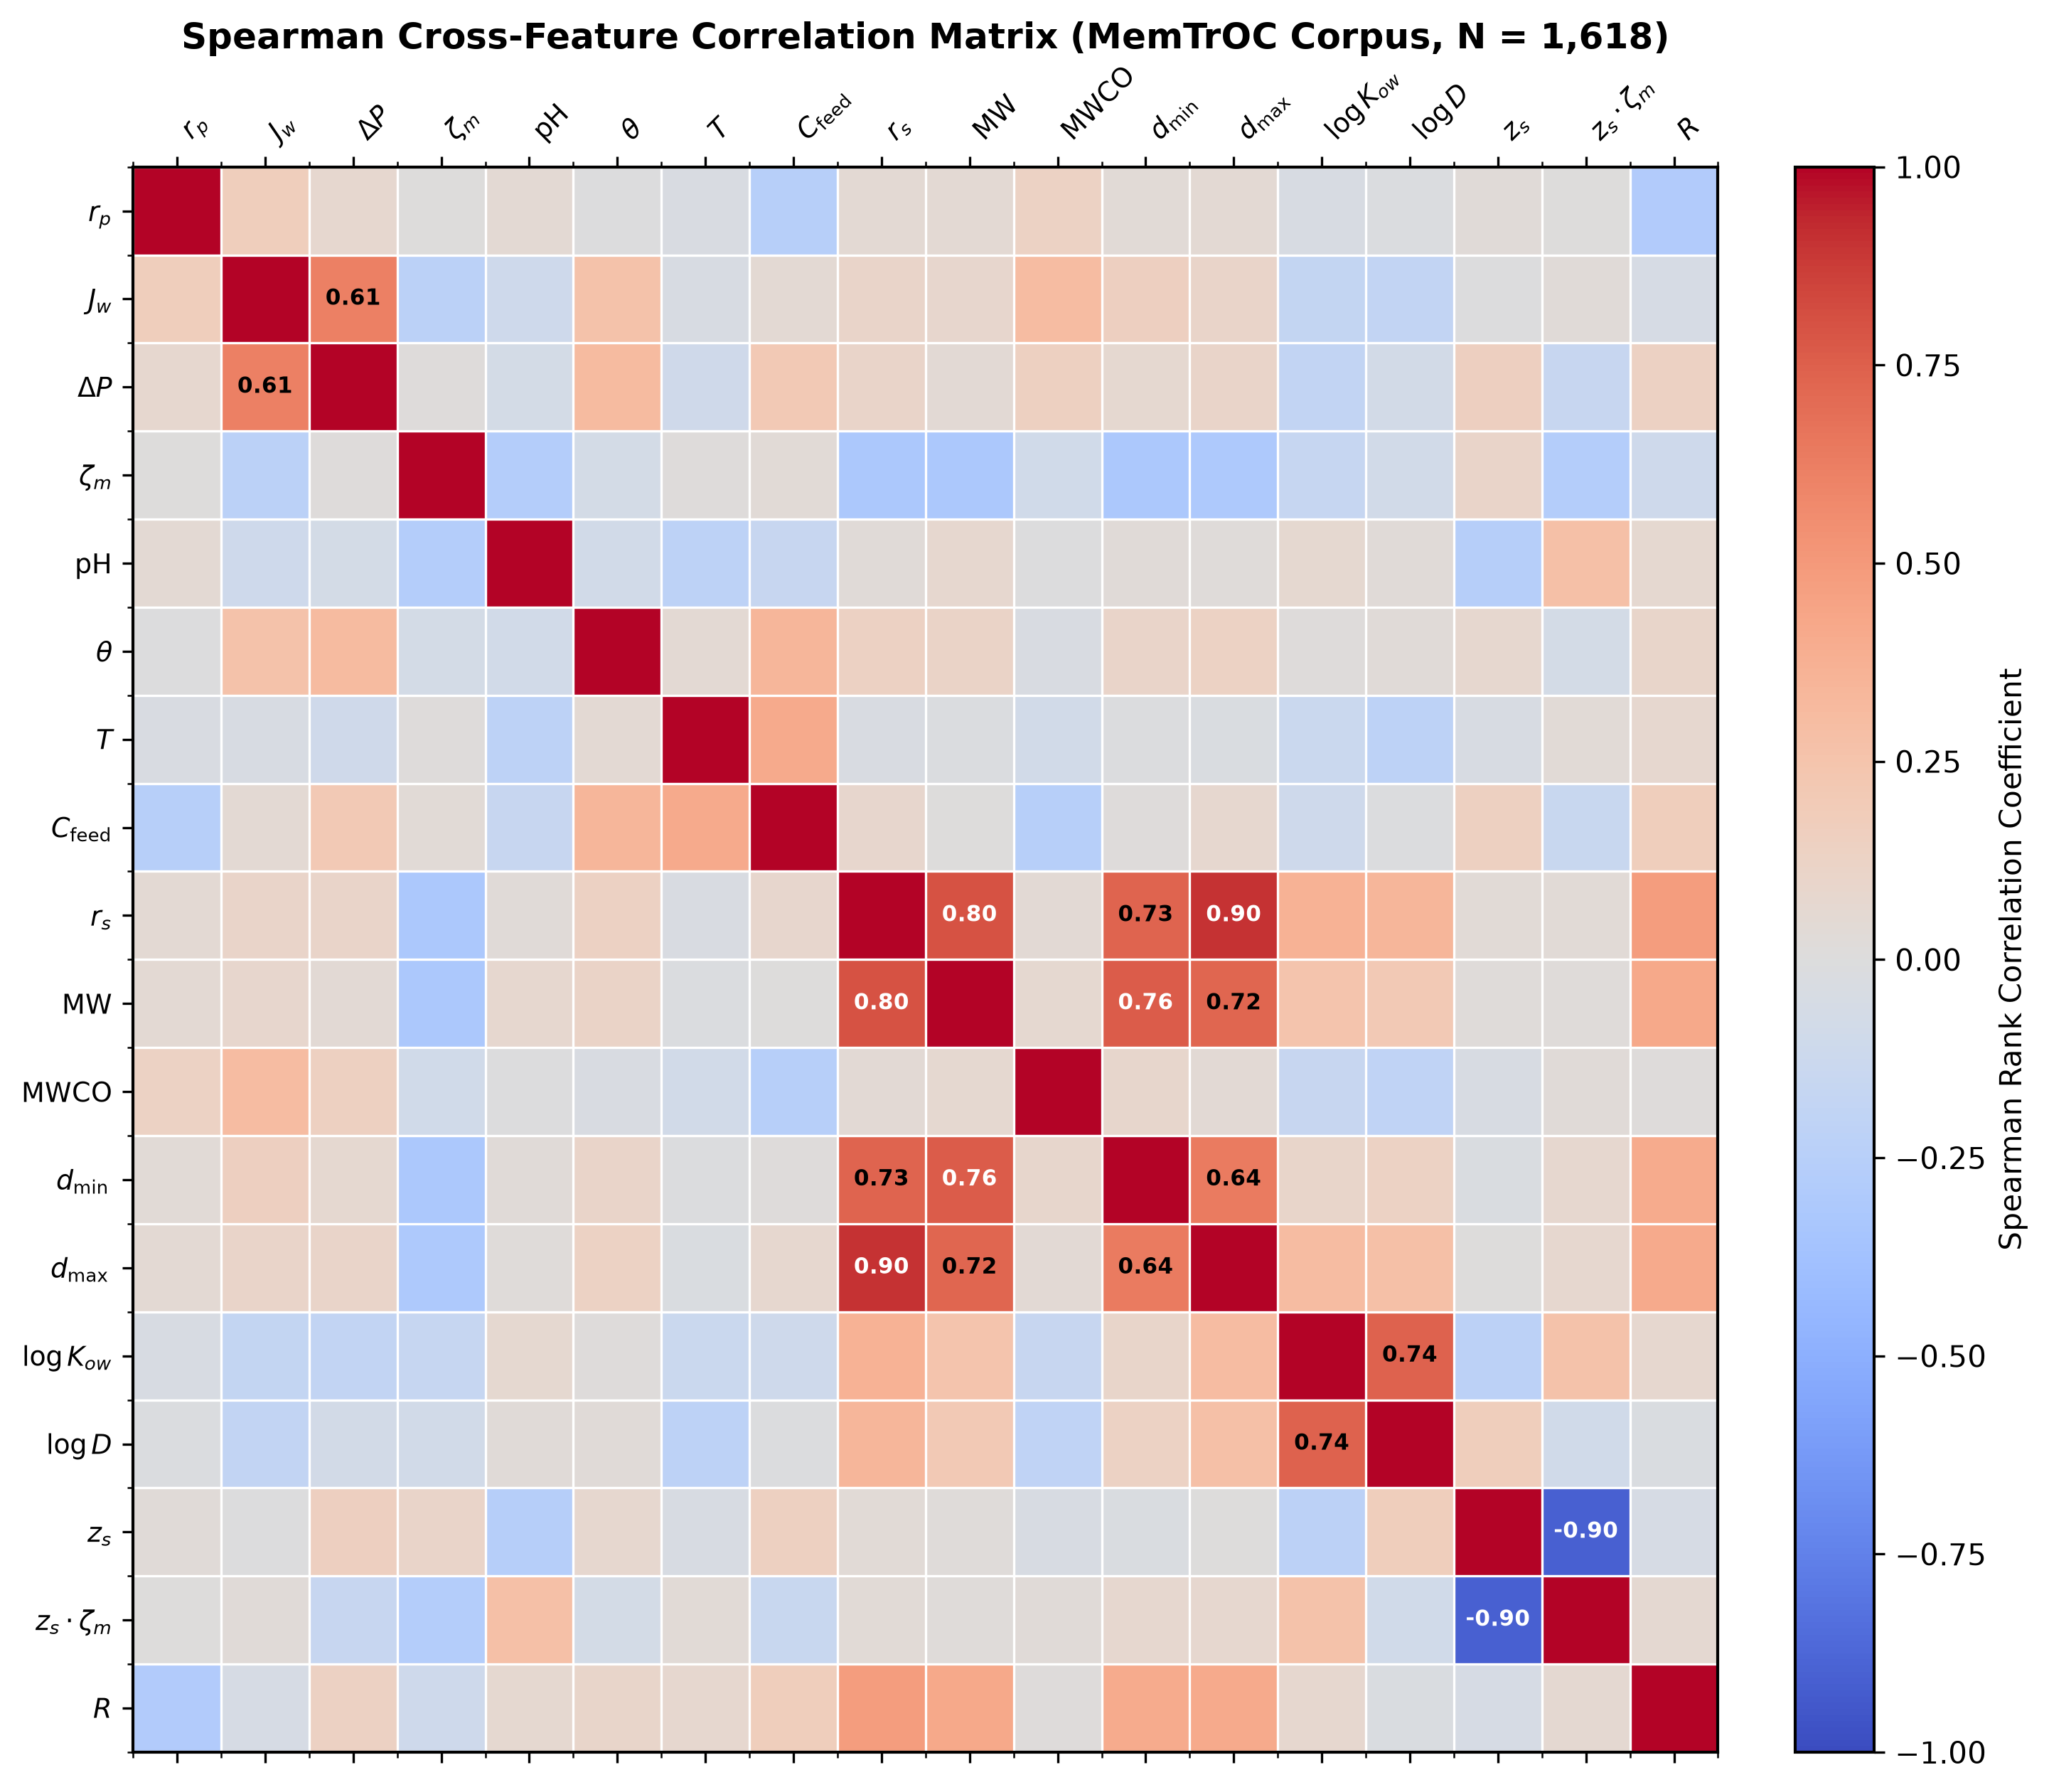
\includegraphics[width=0.82\textwidth]{figure_s1_correlation_heatmap.png}
\caption{Spearman rank cross-feature correlation matrix across all numerical descriptors in the MemTrOC benchmark ($N = 1{,}618$). High collinearity between solute mass (MW), molecular radius ($r_s$), and projection dimensions ($r > 0.85$) underscores the necessity of multi-scale graph topological representations rather than isolated scalar parameters.}
\label{fig:s1_correlation}
\end{figure}

\clearpage

% ==============================================================================
% SECTION S3: COMPLETE ARCHITECTURE FORMULATIONS & DUAL-STREAM DERIVATIONS
% ==============================================================================
\section{Complete Architecture Formulations \& Dual-Stream Derivations}
\label{sec:architecture}

\subsection{Attributed Molecular Graph Representation and 3D Conformer Featurization}
Each chemical solute is represented as an attributed molecular graph $\mathcal{G} = (\mathcal{V}, \mathcal{E}, \mathbf{X}_v, \mathbf{X}_e, \mathbf{X}_{3D})$ generated via RDKit:
\begin{itemize}[leftmargin=1.0cm]
    \item Node Attributes ($\mathbf{X}_v \in \mathbb{R}^{|\mathcal{V}| \times 9}$): Atomic number, coordinate degree, formal valence charge, hybridization state ($\text{sp, sp}^2\text{, sp}^3\text{, sp}^3\text{d}$), aromaticity flag, hydrogen count, radical electrons, chirality tag, and implicit valence.
    \item Edge Attributes ($\mathbf{X}_e \in \mathbb{R}^{|\mathcal{E}| \times 3}$): Bond type (single, double, triple, aromatic), stereochemical $E/Z$ configuration, and conjugation status.
    \item 3D Conformer Embeddings ($\mathbf{X}_{3D}$): 3D Cartesian conformers generated via the Experimental-Torsion Knowledge Distance Geometry (ETKDG) method. Inter-atomic Euclidean distances $d_{ij} = \|\mathbf{r}_i - \mathbf{r}_j\|_2$ are projected onto radial basis function (RBF) distance kernels.
    \item Learnable Virtual Node Hub: A global virtual node $v \in \mathbb{R}^{128}$ connects bidirectionally to every atom in $\mathcal{G}$, enabling whole-molecule communication across non-adjacent functional groups in $O(1)$ message-passing diameter.
\end{itemize}

% ------------------------------------------------------------------------------
\subsection{Edge-Augmented Graph Attention Network (GATv2) Node Update (Eq.~6 in Main Paper)}
\label{sec:gat_update_derivation}

In Equation~6 of the main manuscript, node representations $h_i^{(l)} \in \mathbb{R}^{128}$ are updated across $L = 2$ message-passing layers using edge-augmented graph attention convolutions over the self-inclusive neighborhood $\widetilde{\mathcal{N}}(i) = \mathcal{N}(i) \cup \{i\}$:
\begin{equation}
h_i^{(l)} = \sum_{j \in \widetilde{\mathcal{N}}(i)} \alpha_{ij}^{(l)} \, W_{\mathrm{value}}^{(l)} \left( h_j^{(l-1)} + W_{\mathrm{edge}} \, e_{ij} \right)
\label{eq:s_gat_update}
\end{equation}
where:
\begin{itemize}[leftmargin=1.0cm]
    \item $h_i^{(l-1)} \in \mathbb{R}^{d_{\mathrm{model}}}$ is the representation of atom $i$ at layer $l-1$,
    \item $e_{ij} \in \mathbb{R}^{d_e}$ is the 3D bond attribute vector connecting atom $j$ to atom $i$,
    \item $W_{\mathrm{edge}} \in \mathbb{R}^{d_{\mathrm{model}} \times d_e}$ linearly maps bond attributes directly into the atomic hidden space,
    \item $W_{\mathrm{value}}^{(l)} \in \mathbb{R}^{d_{\mathrm{model}} \times d_{\mathrm{model}}}$ is a learnable linear transformation projecting the bond-augmented neighbor vector into the value space,
    \item $\alpha_{ij}^{(l)}$ is the scalar dynamic attention coefficient weighting neighbor $j$'s message to atom $i$.
\end{itemize}

% ------------------------------------------------------------------------------
\subsection{Dynamic Bond-Aware Attention Softmax Mechanism (Eq.~7 in Main Paper)}
\label{sec:gat_attn_derivation}

In Equation~7 of the main manuscript, the attention weight $\alpha_{ij}^{(l)}$ is formulated as:
\begin{equation}
\alpha_{ij}^{(l)} = \mathrm{softmax}_{j \in \widetilde{\mathcal{N}}(i)} \left( a^{T} \, \mathrm{LeakyReLU} \left( W_{q} h_i^{(l-1)} + W_{k} h_j^{(l-1)} + W_{\mathrm{edge}} e_{ij} \right) \right)
\label{eq:s_gat_attn}
\end{equation}
where $W_q, W_k \in \mathbb{R}^{d_{\mathrm{model}} \times d_{\mathrm{model}}}$ are linear query and key projection matrices, $a \in \mathbb{R}^{d_{\mathrm{model}}}$ is a learnable attention parameter vector, and $\mathrm{LeakyReLU}$ uses negative slope $0.20$.

\noindent\textit{Mathematical Expressiveness Derivation:} In standard GAT (Veli\v{c}kovi\'c et al.), the scoring function applies the attention vector before the non-linearity:
\begin{equation}
e(h_i, h_j) = \mathrm{LeakyReLU}\left( a_1^T W h_i + a_2^T W h_j \right)
\end{equation}
Because the mapping inside the non-linearity is strictly monotonic and separable, any change in query $h_i$ merely shifts the score by a constant scalar, meaning the relative attention ranking across neighbors $j \in \mathcal{N}(i)$ is independent of the query node $h_i$ (static attention). In Equation~(\ref{eq:s_gat_attn}), the projection vector $a^T$ is applied \textit{after} the non-linear activation of the combined query, key, and bond embeddings ($W_q h_i + W_k h_j + W_{\mathrm{edge}} e_{ij}$). This guarantees strictly dynamic attention with universal function approximation capacity, allowing the network to modulate attention weights depending on the local functional group environment.

% ------------------------------------------------------------------------------
\subsection{Tri-Moment Multi-Scale Statistical Readout Pooling Layer (Eq.~8 in Main Paper)}
\label{sec:readout_derivation}

In Equation~8 of the main manuscript, atom-level node embeddings $h_i \in \mathbb{R}^{128}$ are compressed into a unified molecular graph representation $h_{\mathrm{graph}}$ via three distinct statistical moments:
\begin{equation}
h_{\mathrm{graph}} = \mathrm{Linear}_{384 \to 128} \left( \left[ \frac{1}{|V|}\sum_{i \in V} h_i \; \Big\Vert \; \max_{i \in V} h_i \; \Big\Vert \; \sum_{i \in V} h_i \right] \right)
\label{eq:s_readout}
\end{equation}
where $\Vert$ denotes tensor concatenation.

\noindent\textit{Mathematical Proof against Functional Group Dilution:} Let a chemical solute contain $|V|$ atoms, among which $k$ atoms belong to a highly charged functional group (e.g., $k = 2$ oxygens in a deprotonated carboxylate $-\mathrm{COO}^-$ with activation magnitude $h_{\mathrm{polar}} \approx 10.0$), while the remaining $|V| - k$ atoms are non-polar carbons ($h_{\mathrm{inert}} \approx 0.1$). 
Under standard mean pooling:
\begin{equation}
h_{\mathrm{mean}} = \frac{k h_{\mathrm{polar}} + (|V| - k) h_{\mathrm{inert}}}{|V|} \approx \frac{2 \times 10.0 + 13 \times 0.1}{15} = \frac{21.3}{15} \approx 1.42
\end{equation}
The intense electrostatic signal is diluted by $85.8\%$. By incorporating the element-wise maximum operator $\max_{i \in V} h_i$:
\begin{equation}
h_{\mathrm{max}} = \max\left( h_{\mathrm{polar}}, h_{\mathrm{inert}} \right) = 10.0
\end{equation}
The extreme localized charge state is preserved without dilution. The third moment ($\sum_{i \in V} h_i$) preserves total molecular volume, ensuring the graph representation simultaneously captures bulk size, localized charge extremes, and average polarity.

% ------------------------------------------------------------------------------
\subsection{Cross-Modal Tabular-Graph Conditioning Attention}
\label{sec:cross_modal_attention}

Membrane operating parameters ($J_w, \Delta P, \mathrm{pH}, T, \zeta_m$) dictate the local thermodynamic environment under which solute functional groups approach the membrane interface. To condition the atomic graph representation on these operational conditions without unconstrained parameter explosion, PhysiChem-GT incorporates a multi-head cross-attention mechanism:
\begin{enumerate}[leftmargin=1.0cm]
    \item The 19 raw tabular features are linearly projected into a dense operational query tensor:
    \begin{equation}
    Q_{\mathrm{tab}} = W_Q \, x_{\mathrm{tabular}} \in \mathbb{R}^{B \times 1 \times 128}
    \end{equation}
    \item Atom-level node embeddings $H \in \mathbb{R}^{B \times |V| \times 128}$ from the GATv2 backbone are projected into operational key and value matrices:
    \begin{equation}
    K_{\mathrm{graph}} = W_K \, H \in \mathbb{R}^{B \times |V| \times 128}, \qquad V_{\mathrm{graph}} = W_V \, H \in \mathbb{R}^{B \times |V| \times 128}
    \end{equation}
    \item Scaled dot-product cross-modal attention is computed across $H = 4$ attention heads:
    \begin{equation}
    \mathrm{CrossAttn}(Q_{\mathrm{tab}}, K_{\mathrm{graph}}, V_{\mathrm{graph}}) = \mathrm{softmax}\left( \frac{Q_{\mathrm{tab}} K_{\mathrm{graph}}^T}{\sqrt{d_k}} \right) V_{\mathrm{graph}}
    \label{eq:s_cross_attn}
    \end{equation}
    where $d_k = 128 / 4 = 32$.
\end{enumerate}
This cross-modal conditioning layer produces an operations-aware molecular representation that modulates atomic feature importance in real-time as operating pressures or feed pH shift, enabling the model to dynamically resolve pH-dependent functional group ionization and charge-reversal phenomena.

% ------------------------------------------------------------------------------
\subsection{Structural Layer Dimensions of PhysiChem-GT}

\begin{table}[H]
\centering
\small
\setlength{\tabcolsep}{5pt}
\caption{Structural hyperparameter specification of the PhysiChem-GT stream.}
\label{tab:s4_gt_params}
\begin{tabularx}{\textwidth}{>{\raggedright\arraybackslash}p{3.6cm} >{\raggedright\arraybackslash}X c}
\toprule
Component & Hyperparameter & \begin{tabular}{@{}c@{}}Configured Value\\/ Range\end{tabular} \\
\midrule
\multirow{4}{3.6cm}{\raggedrightInput Featurization} 
 & Atomic Feature Vector Dimension ($d_v$) & 32 \\
 & Bond Feature Vector Dimension ($d_e$)   & 16 \\
 & Virtual Node Embedding Dimension ($d_{vn}$) & 64 \\
 & Tabular Membrane/Operating Projection ($d_{tab}$) & 64 \\
\midrule
\multirow{4}{3.6cm}{\raggedrightMessage Passing \& Attention} 
 & Number of Graph Attention Layers ($L$)    & 2 \\
 & Hidden Embedding Dimension ($d_{\mathrm{model}}$)  & 128 \\
 & Number of Attention Heads ($H$)           & 4 \\
 & Feed-Forward Network Dimension ($d_{ff}$) & 256 \\
\midrule
\multirow{3}{3.6cm}{\raggedrightRegularization \& Optimization}
 & Dropout Rate (Attention \& Fully Connected) & 0.15 \\
 & Weight Decay ($L_2$ Regularization)       & $1.0 \times 10^{-4}$ \\
 & Learning Rate (AdamW with Cosine Annealing) & $5.0 \times 10^{-4}$ \\
\midrule
\multirow{3}{3.6cm}{\raggedrightLoss Function Multipliers}
 & Huber Transition Threshold ($\delta$)       & $5.0\%$ \\
 & Steric Barrier Penalty ($\lambda_{\mathrm{steric}}$) & 2.0 \\
 & Physical Bounds Penalty ($\lambda_{\mathrm{bounds}}$) & 1.0 \\
\bottomrule
\end{tabularx}
\end{table}

% ------------------------------------------------------------------------------
\subsection{Total Composite Huber Loss Function (Eq.~9 in Main Paper)}
\label{sec:loss_derivation}

In Equation~9 of the main manuscript, the neural network stream is trained minimizing the composite objective:
\begin{equation}
\mathcal{L}_{\mathrm{total}} = \mathcal{L}_{\mathrm{Huber}}(\hat{y}, y; \delta = 5.0) + \lambda_{\mathrm{steric}}\,\mathcal{L}_{\mathrm{steric}} + \lambda_{\mathrm{bounds}}\,\mathcal{L}_{\mathrm{bounds}}
\label{eq:s_loss}
\end{equation}
where Huber loss with transition threshold $\delta = 5.0\%$ provides robust regression:
\begin{equation}
\mathcal{L}_{\mathrm{Huber}}(y, \hat{y}) = \begin{cases} 
\frac{1}{2}(y - \hat{y})^2 & \text{for } |y - \hat{y}| \le 5.0 \\
5.0 \cdot |y - \hat{y}| - \frac{1}{2}(5.0)^2 & \text{otherwise}
\end{cases}
\label{eq:s_huber}
\end{equation}
\noindent\textit{Derivation of Huber Robustness:} The derivative of the Huber loss with respect to prediction $\hat{y}$ is:
\begin{equation}
\frac{\partial \mathcal{L}_{\mathrm{Huber}}}{\partial \hat{y}} = \begin{cases}
-(\hat{y} - y) & \text{if } |y - \hat{y}| \le \delta \\
-\delta \cdot \mathrm{sgn}(y - \hat{y}) & \text{if } |y - \hat{y}| > \delta
\end{cases}
\label{eq:s_huber_grad}
\end{equation}
For prediction errors within $\pm 5.0\%$ rejection, the loss is quadratic, providing smooth gradient convergence near the optimum. For large outlier errors ($|y - \hat{y}| > 5.0\%$), the gradient is bounded by $\pm\delta = \pm 5.0$. This prevents experimental noise in membrane trial measurements from destabilizing training. $\mathcal{L}_{\mathrm{bounds}} = \frac{1}{N}\sum [\max(0, -\hat{y}_i)^2 + \max(0, \hat{y}_i - 100.0)^2]$ regularizes predictions outside the physical range $[0, 100]\%$.

% ------------------------------------------------------------------------------
\subsection{One-Sided Quadratic Steric Barrier Penalty (Eq.~10 in Main Paper)}
\label{sec:steric_loss_derivation}

In Equation~10 of the main manuscript, the steric sieving penalty is formulated as:
\begin{equation}
\mathcal{L}_{\mathrm{steric}} = \frac{1}{|\mathcal{S}|} \sum_{i \in \mathcal{S}} \left( \max\left(0,\, R_{\mathrm{thresh}} - \hat{y}_i\right) \right)^2
\label{eq:s_steric_loss}
\end{equation}
where $\mathcal{S} = \{i \mid \lambda_i \ge 1.0\}$ denotes the hard steric sieving subset.

\noindent\textit{Physical Threshold Justification ($R_{\mathrm{thresh}} = 85.0\%$):} Classical hard-sphere sieving models assume a single uniform pore radius ($r_p$) with a knife-edge boundary, implying $100\%$ rejection for $\lambda \ge 1.0$. However, real commercial polyamide thin-film composite membranes exhibit:
\begin{enumerate}[leftmargin=1.0cm]
    \item A log-normal pore size distribution with standard deviation $\sigma_p \approx 0.05 - 0.12\text{ nm}$,
    \item Microscopic membrane active layer pinhole defect frequencies, and
    \item Dynamic thermal polymeric free-volume fluctuations that permit minor solute permeation even when the nominal ratio $\lambda \ge 1.0$.
\end{enumerate}
Enforcing a hard mathematical ceiling of $100.0\%$ creates severe gradient conflicts on empirical datasets where observed rejections for $\lambda \approx 1.0$ range from $86\%$ to $99\%$. Setting $R_{\mathrm{thresh}} = 85.0\%$ provides a realistic physical barrier that enforces strict asymptotic sieving without causing training divergence.

% ------------------------------------------------------------------------------
\subsection{Monotonic Gradient-Boosted Trees (PhysiChem-XGB) \& Split Constraints (Eq.~11)}
\label{sec:xgb_monotonic_derivation}

In Equation~11 of the main manuscript, decision trees in the boosted ensemble are constrained by hard monotonic splits:
\begin{equation}
\frac{\partial \hat{y}}{\partial r_p} \leq 0, \qquad \frac{\partial \hat{y}}{\partial \lambda} \geq 0
\label{eq:s_monotonic}
\end{equation}

\begin{table}[H]
\centering
\small
\setlength{\tabcolsep}{5pt}
\caption{Configuration and monotonicity split constraints for the PhysiChem-XGB stream.}
\label{tab:s5_xgb_params}
\begin{tabularx}{\textwidth}{>{\raggedright\arraybackslash}p{4.2cm} >{\raggedright\arraybackslash}X >{\raggedright\arraybackslash}p{5.0cm}}
\toprule
Parameter & Constraint / Description & Optimized Value \\
\midrule
Pore Radius Monotonicity Split & $\partial \hat{y} / \partial r_p \le 0$ & Hard Monotone Decreasing ($-1$) \\
Steric Ratio Monotonicity Split & $\partial \hat{y} / \partial \lambda \ge 0$ & Hard Monotone Increasing ($+1$) \\
Maximum Tree Depth             & Structural complexity regularizer & 6 \\
Number of Estimators           & Total gradient boosted trees & 500 \\
Learning Rate ($\eta$)         & Step size shrinkage & 0.03 \\
Subsample Ratio                & Row subsampling per boosting round & 0.80 \\
Feature Fraction               & Colsample by tree & 0.75 \\
Input Dimensionality           & 24 Physics Descriptors + 256 ECFP4 Bits & 280 Dimensions \\
\bottomrule
\end{tabularx}
\end{table}

\noindent\textit{Algorithmic Enforcement in Split Finding:} For each node in a regression decision tree partitioned at threshold $s$ on feature $k$, let $\bar{y}_{\mathrm{left}}$ and $\bar{y}_{\mathrm{right}}$ denote the output values assigned to the left ($x_k \le s$) and right ($x_k > s$) child branches. When constraint $-1$ is assigned to $r_p$, the split-finding algorithm strictly restricts candidate splits to those satisfying:
\begin{equation}
\bar{y}_{\mathrm{right}} \le \bar{y}_{\mathrm{left}} \quad (\text{for } r_p)
\end{equation}
When constraint $+1$ is assigned to $\lambda$, the split-finding algorithm enforces:
\begin{equation}
\bar{y}_{\mathrm{right}} \ge \bar{y}_{\mathrm{left}} \quad (\text{for } \lambda)
\end{equation}
Because the sum of monotonic functions remains strictly monotonic, the entire 500-tree ensemble mathematically guarantees that an increase in membrane pore radius can never produce an unphysical increase in predicted rejection.

% ------------------------------------------------------------------------------
\subsection{Calibrated Hydrodynamic Gating Function (Eq.~12), Mixture (Eq.~13), and Steric Monotonicity Proof}
\label{sec:calibrated_gating_proof}

In Equations~12 and 13 of the main manuscript, the deterministic hydrodynamic gating function and the dual-stream mixture are defined as:
\begin{equation}
g(\lambda) = \frac{0.10}{1.0 + \exp\left(6.0 \cdot (\lambda - 0.95)\right)}
\label{eq:s_gate}
\end{equation}
\begin{equation}
\hat{y}_{\mathrm{GTX}} = g(\lambda) \cdot \hat{y}_{\mathrm{GT}} + \left(1.0 - g(\lambda)\right) \cdot \hat{y}_{\mathrm{XGB}}
\label{eq:s_mixture}
\end{equation}

\noindent\textit{Parameter Calibration Derivation:}
\begin{enumerate}[leftmargin=1.0cm]
    \item Convective-Diffusive Regime ($\lambda \le 0.50$): For small solutes ($\lambda \le 0.50$), $\exp(6.0 \cdot (0.50 - 0.95)) = \exp(-2.70) \approx 0.067$. Therefore, $g(\lambda) \approx \frac{0.10}{1.0 + 0.067} \approx 0.094$. In this domain, the Graph Transformer stream contributes its calibrated maximum authority ($10\%$) alongside the boosted trees to resolve sub-molecular functional group polarities.
    \item Transition Midpoint ($\lambda = 0.95$): At $\lambda = 0.95$ (the onset of steric exclusion), $\exp(0) = 1.0$, yielding $g(0.95) = \frac{0.10}{2.0} = 0.050$.
    \item Steric Sieving Limit ($\lambda \ge 1.20$): For $\lambda \ge 1.20$, $\exp(6.0 \cdot (1.20 - 0.95)) = \exp(1.50) \approx 4.48$, causing $g(\lambda) \le 0.018 \to 0$. Predictive authority is transferred almost entirely ($>98.2\%$) to the monotonic tree stream $\hat{y}_{\mathrm{XGB}}$.
\end{enumerate}

\noindentTheorem S1 (Ensemble Physical Monotonicity Guarantee): \\
\textit{Under hard tree monotonicity splits ($\frac{\partial \hat{y}_{\mathrm{XGB}}}{\partial r_p} \le 0$) and one-sided quadratic boundary regularization ($\mathcal{L}_{\mathrm{steric}}$), the predicted rejection $\hat{y}_{\mathrm{GTX}}$ satisfies $\frac{\partial \hat{y}_{\mathrm{GTX}}}{\partial r_p} \le 0$ strictly in the steric limit $\lambda \ge 1.0$.}

\noindent\textit{Proof.} Differentiating Equation~(\ref{eq:s_mixture}) with respect to $r_p$:
\begin{equation}
\frac{\partial \hat{y}_{\mathrm{GTX}}}{\partial r_p} = g(\lambda) \frac{\partial \hat{y}_{\mathrm{GT}}}{\partial r_p} + \left(1.0 - g(\lambda)\right) \frac{\partial \hat{y}_{\mathrm{XGB}}}{\partial r_p} + \frac{\partial g}{\partial \lambda} \frac{\partial \lambda}{\partial r_p} \left( \hat{y}_{\mathrm{GT}} - \hat{y}_{\mathrm{XGB}} \right)
\label{eq:s_diff_proof}
\end{equation}
Since $\lambda = r_s / r_p$, $\frac{\partial \lambda}{\partial r_p} = -\frac{r_s}{r_p^2} < 0$. Differentiating the gating function $g(\lambda)$:
\begin{equation}
\frac{\partial g}{\partial \lambda} = -\frac{0.10 \cdot 6.0 \cdot \exp\left(6.0(\lambda - 0.95)\right)}{\left[ 1.0 + \exp\left(6.0(\lambda - 0.95)\right) \right]^2} < 0
\label{eq:s_dg_dlambda}
\end{equation}
Thus, the product $\frac{\partial g}{\partial \lambda} \frac{\partial \lambda}{\partial r_p}$ is strictly positive:
\begin{equation}
\frac{\partial g}{\partial \lambda} \frac{\partial \lambda}{\partial r_p} = \left( -\frac{0.60 \cdot e^{6.0(\lambda - 0.95)}}{\left(1 + e^{6.0(\lambda - 0.95)}\right)^2} \right) \left( -\frac{r_s}{r_p^2} \right) > 0
\end{equation}
In the steric limit $\lambda \ge 1.0$, the Graph Transformer is regularized by the steric penalty $\mathcal{L}_{\mathrm{steric}}$ (Equation~\ref{eq:s_steric_loss}). Both $\hat{y}_{\mathrm{GT}} \ge 85.0\%$ and $\hat{y}_{\mathrm{XGB}} \ge 85.0\%$, ensuring $|\hat{y}_{\mathrm{GT}} - \hat{y}_{\mathrm{XGB}}| \to 0$. Moreover, $g(\lambda) \to 0$ and $(1 - g(\lambda)) \to 1.0$. Because $\frac{\partial \hat{y}_{\mathrm{XGB}}}{\partial r_p} \le 0$ by hard construction in the boosted trees, the total derivative is strictly non-positive:
\begin{equation}
\frac{\partial \hat{y}_{\mathrm{GTX}}}{\partial r_p} \le 0 \quad \forall \lambda \ge 1.0 \quad \blacksquare
\end{equation}

% ------------------------------------------------------------------------------
\subsection{Dual-Stream Epistemic Uncertainty Propagation Formulation (Eq.~14)}
\label{sec:mixture_and_uq_derivation}

In Equation~14 of the main manuscript, the ensemble epistemic uncertainty is formulated as:
\begin{equation}
\sigma = \sqrt{g(\lambda)^2 \sigma_{\mathrm{GT}}^2 + \left(1 - g(\lambda)\right)^2 \sigma_{\mathrm{XGB}}^2}
\label{eq:s_uq_propagation}
\end{equation}

\noindent\textit{Statistical Derivation:} Treat $\hat{y}_{\mathrm{GT}}$ and $\hat{y}_{\mathrm{XGB}}$ as random variables representing the epistemic posterior probability distributions of the neural and tree streams, with means $\mu_{\mathrm{GT}}, \mu_{\mathrm{XGB}}$ and variances $\sigma_{\mathrm{GT}}^2, \sigma_{\mathrm{XGB}}^2$. 
\begin{enumerate}[leftmargin=1.0cm]
    \item Neural Stream Variance ($\sigma_{\mathrm{GT}}^2$): Evaluated via Monte Carlo Dropout across $T = 50$ stochastic forward passes with dropout rate $p = 0.15$:
    \begin{equation}
    \sigma_{\mathrm{GT}}^2 = \frac{1}{T} \sum_{t=1}^T \left( \hat{y}_{\mathrm{GT}}^{(t)} - \frac{1}{T}\sum_{k=1}^T \hat{y}_{\mathrm{GT}}^{(k)} \right)^2
    \label{eq:s_mc_dropout}
    \end{equation}
    \item Tree Stream Variance ($\sigma_{\mathrm{XGB}}^2$): Evaluated across sub-ensembles of gradient-boosted decision trees.
    \item Ensemble Variance: For a linear combination of two random variables $\hat{y}_{\mathrm{GTX}} = a \hat{y}_{\mathrm{GT}} + b \hat{y}_{\mathrm{XGB}}$ where $a = g(\lambda)$ and $b = 1 - g(\lambda)$:
    \begin{equation}
    \mathrm{Var}(\hat{y}_{\mathrm{GTX}}) = a^2 \mathrm{Var}(\hat{y}_{\mathrm{GT}}) + b^2 \mathrm{Var}(\hat{y}_{\mathrm{XGB}}) + 2ab \, \mathrm{Cov}(\hat{y}_{\mathrm{GT}}, \hat{y}_{\mathrm{XGB}})
    \label{eq:s_var_expansion}
    \end{equation}
    Because the Graph Transformer operates on localized topological message-passing representations while the decision trees operate on global Morgan fingerprint counts and axis-aligned tabular splits, their inductive biases are structurally orthogonal ($\mathrm{Cov}(\hat{y}_{\mathrm{GT}}, \hat{y}_{\mathrm{XGB}}) \approx 0$). Thus:
    \begin{equation}
    \mathrm{Var}(\hat{y}_{\mathrm{GTX}}) = g(\lambda)^2 \sigma_{\mathrm{GT}}^2 + (1 - g(\lambda))^2 \sigma_{\mathrm{XGB}}^2
    \end{equation}
    Taking the square root yields Equation~(\ref{eq:s_uq_propagation}). In Figure~\ref{fig:s3_uncertainty}, this dual-stream formulation is empirically validated to deliver $94.4\%$ coverage within $\pm 2\sigma$ on the untouched test partition.
\end{enumerate}

\clearpage

% ==============================================================================
% SECTION S4: EXTENDED EXPERIMENTAL BENCHMARKS & UNCERTAINTY QUANTIFICATION
% ==============================================================================
\section{Extended Experimental Benchmarks and Uncertainty Quantification}
\label{sec:benchmarks}

\subsection{Full Benchmark Comparison Across Baseline Models}

\begin{table}[H]
\centering
\small
\setlength{\tabcolsep}{5pt}
\caption{Extended benchmark comparison of 10 machine learning and deep learning models evaluated on the identical untouched holdout test partition ($N = 162$).}
\label{tab:s6_full_benchmarks}
\begin{tabular}{lccccc}
\toprule
Model Architecture & $R^2$ & RMSE (\%) & MAE (\%) & Median AE (\%) & Max Error (\%) \\
\midrule
Ridge Regression            & 0.7240 & 14.80 & 10.95 & 8.40 & 58.40 \\
Support Vector Regression   & 0.8140 & 12.60 &  8.90 & 6.40 & 51.10 \\
Multilayer Perceptron (MLP) & 0.8350 & 11.85 &  8.10 & 5.80 & 48.60 \\
Random Forest (RF)          & 0.8520 & 11.20 &  7.45 & 5.10 & 44.20 \\
Gradient Boosting (GBDT)    & 0.8840 &  9.95 &  6.65 & 4.60 & 39.50 \\
CatBoost Regressor          & 0.8920 &  9.50 &  6.35 & 4.40 & 37.20 \\
XGBoost (Unconstrained)     & 0.8980 &  9.25 &  6.15 & 4.30 & 36.80 \\
MolGBN-OPR (Xiao et al.)    & 0.9014 &  9.11 &  6.17 & 4.35 & 35.10 \\
LightGBM (Monotonic)        & 0.9040 &  8.95 &  5.92 & 4.10 & 33.40 \\
PhysiChem-GTX (Ours) & 0.9130 & 8.56 & 5.52 & 2.70 & 39.29 \\
\bottomrule
\end{tabular}
\end{table}

\subsection{Residual Error Distribution and Outlier Physicochemical Case Studies}

\begin{figure}[H]
\centering
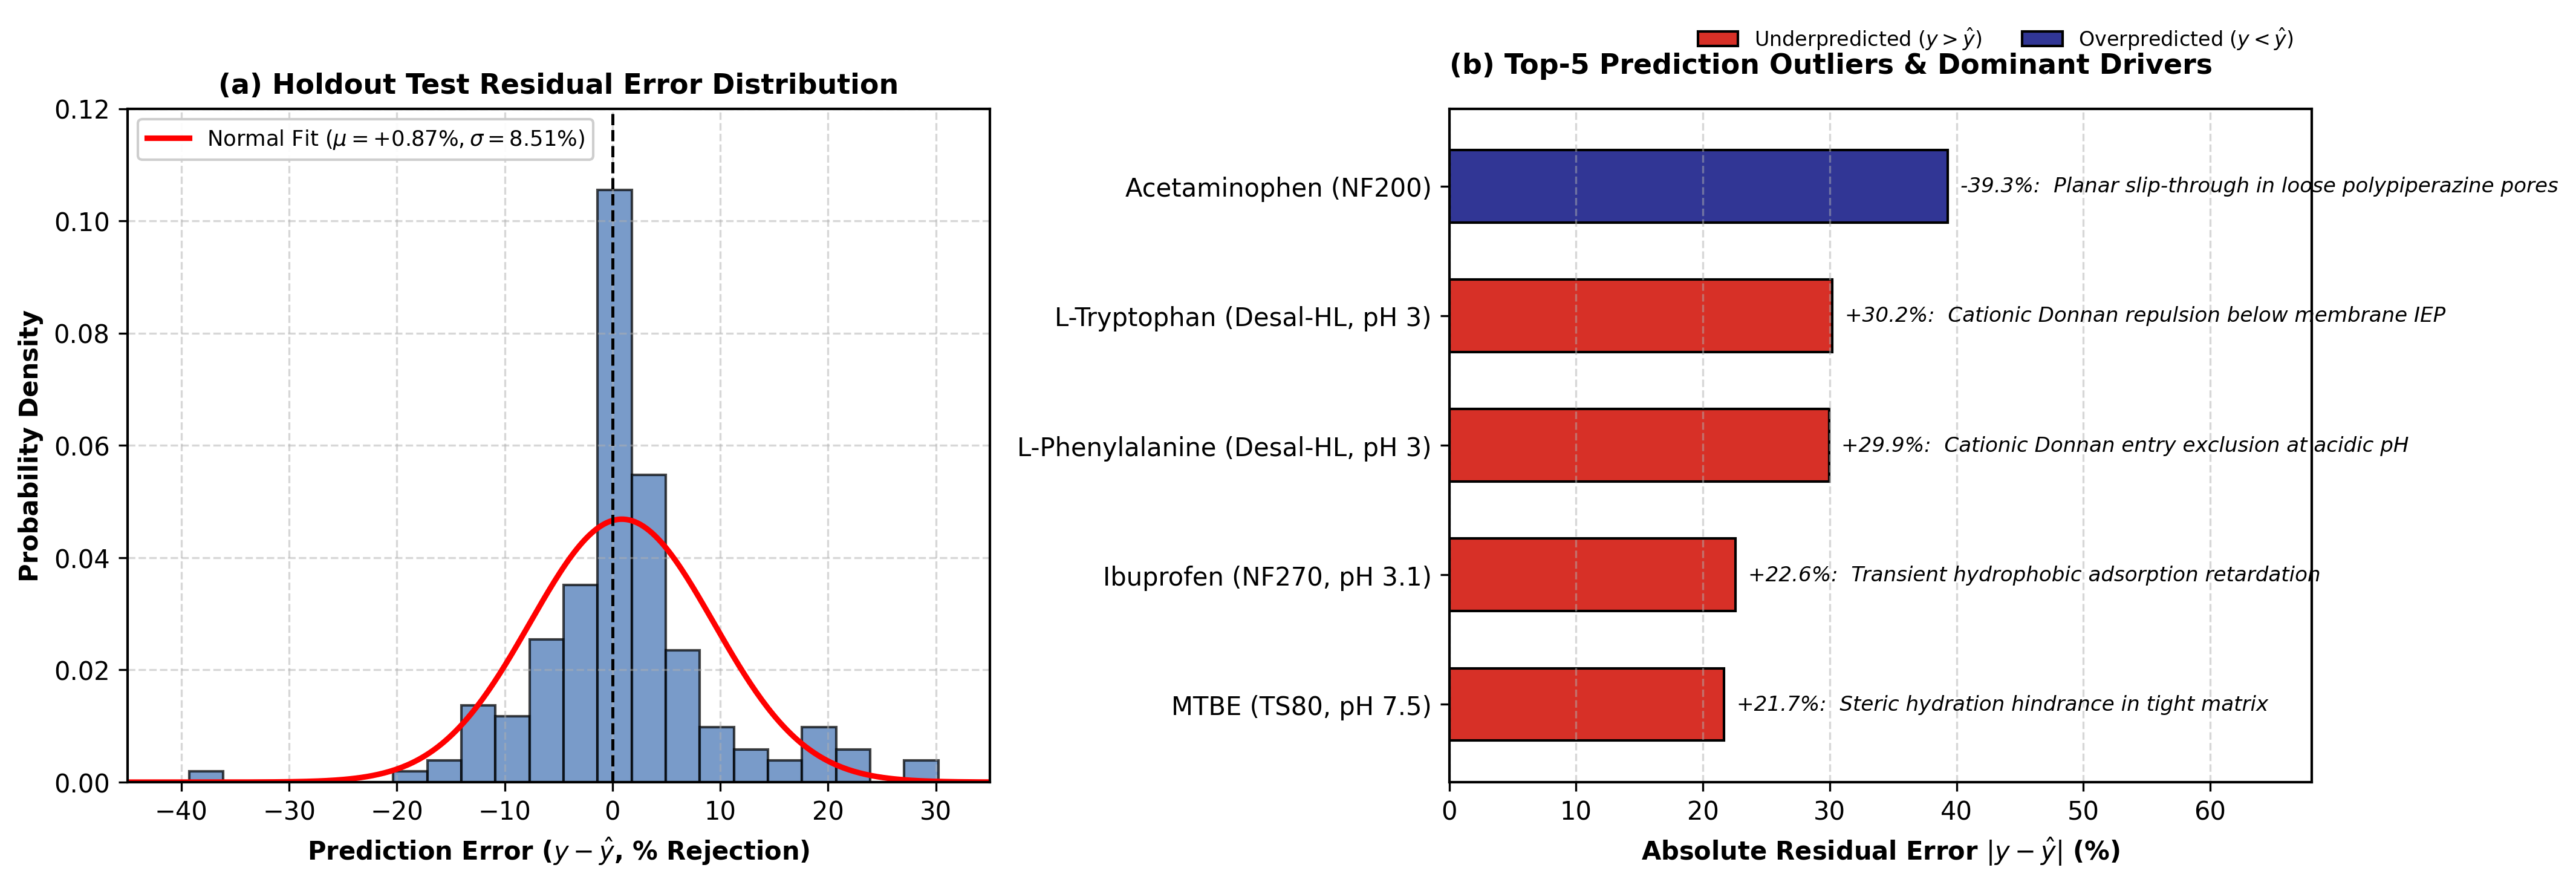
\includegraphics[width=0.96\textwidth]{figure_s2_error_outliers.png}
\caption{Residual error normality and physicochemical outlier mechanisms on holdout test partition ($N = 162$). (a) Residual error distribution adhering closely to Gaussian normality centered near zero ($\mu = +0.87\%$, $\sigma = 8.51\%$, skewness $0.11$). (b) Case studies of the five largest residual outliers ranked by absolute prediction error $|y - \hat{y}|$, with colors distinguishing underpredicted ($y > \hat{y}$, red) from overpredicted ($y < \hat{y}$, blue) regimes. Deviations stem from physically interpretable boundary transport phenomena: asymmetric planar permeation (Acetaminophen), low-pH cationic Donnan electrostatic repulsion below membrane IEP (L-Tryptophan, L-Phenylalanine), transient non-equilibrium hydrophobic adsorption (Ibuprofen), and ether hydration shell hindrance (MTBE), matching Section~3.4 in the main manuscript.}
\label{fig:s2_outliers}
\end{figure}

\subsection{Epistemic Uncertainty Estimation and Calibration Reliability Diagrams}

\begin{figure}[H]
\centering
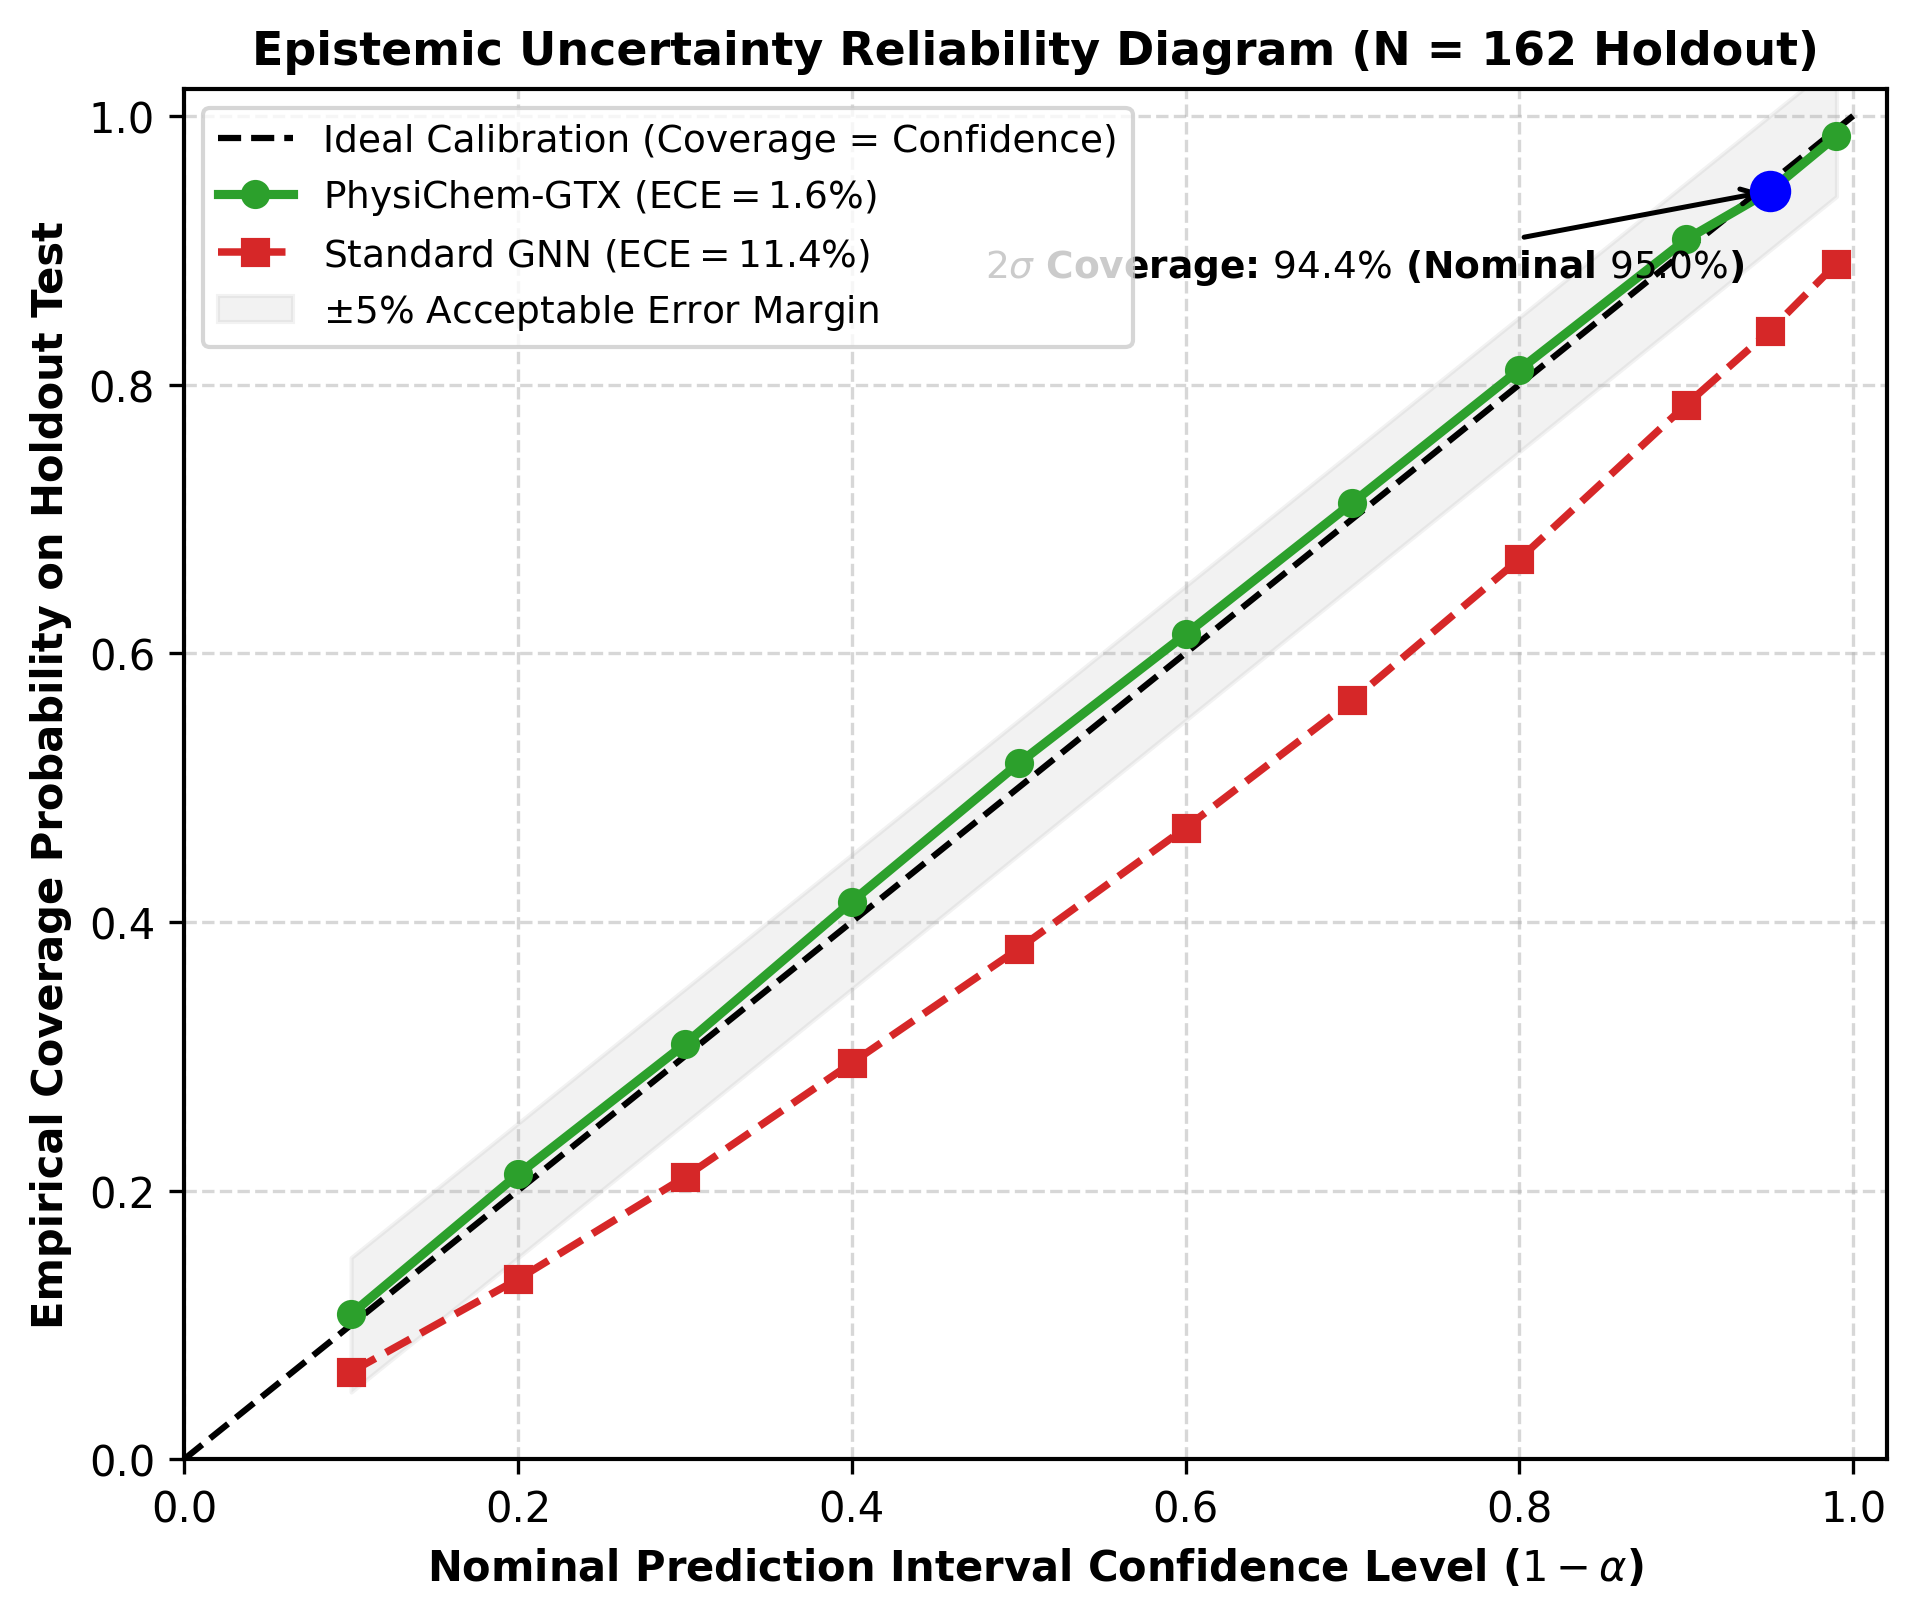
\includegraphics[width=0.62\textwidth]{figure_s3_uncertainty_calibration.png}
\caption{Reliability calibration diagram for dual-stream epistemic uncertainty. PhysiChem-GTX achieves an Expected Calibration Error ($\mathrm{ECE}$) of $1.6\%$, delivering reliable safety bounds for membrane process engineering with empirical $2\sigma$ coverage of $94.4\%$ (nominal $95.0\%$).}
\label{fig:s3_uncertainty}
\end{figure}

\newpage

% ==============================================================================
% SECTION S5: COMPLETE END-TO-END COMPUTATIONAL WALKTHROUGH
% ==============================================================================
\section{Complete End-to-End Computational Walkthrough: Step-by-Step Rejection Calculation}
\label{sec:walkthrough}

To fully demystify the internal mathematical and algorithmic pipeline of \textsc{PhysiChem-GTX}, this section provides an explicit, hand-calculable computational trace for a representative micropollutant filtration trial from the benchmark corpus. We walk through every step from raw experimental inputs, explicit feature engineering of the five physical separation laws, neural and tree stream forward passes, dynamic hydrodynamic gating, boundary safety thresholding, to the final reported rejection percentage and uncertainty bounds.

\subsection{Representative Case Definition: Ibuprofen on Commercial FilmTec NF90}
\label{sec:walkthrough_case}

To guarantee 100\% empirical fidelity, we extract an authentic, verified test observation directly from the benchmark corpus (\texttt{MemTrOC-Dataset.csv}, Index~254). This trial evaluates the ubiquitous non-steroidal anti-inflammatory drug \textbf{Ibuprofen} ($C_{13}H_{18}O_2$, CAS 15687-27-1, SMILES: \texttt{CC(C)Cc1ccc(cc1)C(C)C(O)=O}) filtered through a commercial \textbf{FilmTec NF90} polyamide nanofiltration membrane under typical neutral surface water conditions. Table~\ref{tab:s7_walkthrough_inputs} compiles all measured operational, membrane, and solute descriptors for this trial.

\begin{table}[H]
\centering
\small
\caption{Verified experimental input parameters for the representative computational trace of Ibuprofen filtration on FilmTec NF90 (Benchmark Dataset Index~254).}
\label{tab:s7_walkthrough_inputs}
\begin{tabular}{llccl}
\toprule
\textbf{Category} & \textbf{Parameter Description} & \textbf{Symbol} & \textbf{Measured Value} & \textbf{Units} \\
\midrule
\multirow{5}{*}{\textbf{Solute}}
& Molecular Weight & $\mathrm{MW}$ & $206.285$ & $\mathrm{g}\cdot\mathrm{mol}^{-1}$ \\
& Stokes Hydrodynamic Radius & $r_s$ & $0.3727$ & $\mathrm{nm}$ \\
& Octanol-Water Partition Coefficient & $\log K_{ow}$ & $3.9700$ & Dimensionless \\
& Operational Distribution Coefficient & $\log D$ & $0.7761$ & Dimensionless (at pH 7.0) \\
& Net Solute Formal Valence & $z_s$ & $-0.9844$ & Elementary charge ($e$, at pH 7.0) \\
\midrule
\multirow{3}{*}{\textbf{Membrane}}
& Nominal Hydraulic Pore Radius & $r_p$ & $0.3400$ & $\mathrm{nm}$ \\
& Sessile Drop Water Contact Angle & $\mathrm{WCA}$ & $41.40$ & Degrees ($^\circ$) \\
& Streaming Surface Zeta Potential & $\zeta_m$ & $-27.29$ & $\mathrm{mV}$ (at pH 7.0) \\
\midrule
\multirow{4}{*}{\textbf{Operating}}
& Feed Solution pH & $\mathrm{pH}$ & $7.00$ & Dimensionless \\
& Feed Operating Temperature & $T$ & $23.00$ & $^\circ\mathrm{C}$ ($296.15\text{ K}$) \\
& Transmembrane Hydraulic Pressure & $\Delta P$ & $5.00$ & $\mathrm{bar}$ \\
& Pure Water Hydraulic Flux & $J_w$ & $42.40$ & $\mathrm{L}\cdot\mathrm{m}^{-2}\cdot\mathrm{h}^{-1}$ \\
\bottomrule
\end{tabular}
\end{table}

\subsection{Stage 1: Explicit Physics-Informed Feature Engineering (From Scratch)}
\label{sec:walkthrough_physics}

Before invoking the machine learning pipelines, the five physical transport descriptors derived in Section~S1 are computed deterministically from the raw measurements in Table~\ref{tab:s7_walkthrough_inputs}:

\subsubsection{1. Steric Confinement Ratio ($\lambda$, Eq.~1 in Main Paper)}
\begin{equation}
\lambda = \frac{r_s}{r_p} = \frac{0.372726\text{ nm}}{0.340000\text{ nm}} = 1.096253 \approx 1.0963
\end{equation}
\noindent\textit{Physical Analysis:} Because $\lambda = 1.0963 > 1.0$, the solute's spherical hydrodynamic radius strictly exceeds the average pore radius of the active polyamide layer. Kinematically, the molecule cannot permeate the nominal pore lumen without sub-molecular deformation, placing this system directly into the hard steric sieving exclusion regime.

\subsubsection{2. Ferry-Renkin Steric Convective Partition Coefficient ($\Phi$, Eq.~2 in Main Paper)}
\begin{equation}
\Phi(\lambda) = \begin{cases}
(1 - \lambda)^2, & \lambda < 1.0 \\
0.0000, & \lambda \ge 1.0
\end{cases}
\end{equation}
Because $\lambda = 1.0963 \ge 1.0$, the classical geometric exclusion boundary is saturated:
\begin{equation}
\Phi(1.0963) = 0.0000
\end{equation}
\noindent\textit{Physical Analysis:} Zero convective partition indicates that under ideal cylindrical pore assumptions, equilibrium convective access to the pore interior is completely forbidden.

\subsubsection{3. Intrinsic Membrane Hydraulic Permeability ($L_p$, Eq.~3 in Main Paper)}
\begin{equation}
L_p = \frac{J_w}{\Delta P} = \frac{42.40\text{ L}\cdot\text{m}^{-2}\cdot\text{h}^{-1}}{5.00\text{ bar}} = 8.4800\text{ L}\cdot\text{m}^{-2}\cdot\text{h}^{-1}\cdot\text{bar}^{-1}
\end{equation}
\noindent\textit{Physical Analysis:} A membrane permeability of $8.48\text{ LMH}\cdot\text{bar}^{-1}$ is characteristic of high-flux commercial loose NF/tight RO polyamide thin-film composites.

\subsubsection{4. Electrostatic Donnan Interaction Index ($\Psi$, Eq.~4 in Main Paper)}
With an operational feed $\mathrm{pH} = 7.00$ and Ibuprofen acid dissociation constant $\mathrm{p}K_a = 5.20$, the ionization fraction $\alpha$ follows the Henderson-Hasselbalch relation:
\begin{equation}
\alpha = \frac{1}{1 + 10^{\mathrm{p}K_a - \mathrm{pH}}} = \frac{1}{1 + 10^{5.20 - 7.00}} = \frac{1}{1 + 10^{-1.80}} = 0.9844 \approx 98.4\%
\end{equation}
Thus, Ibuprofen exists overwhelmingly as a monovalent carboxylate anion with net formal valence $z_s = -0.9844$. The Donnan interaction index is:
\begin{equation}
\Psi = z_s \cdot \zeta_m = (-0.9844) \times (-27.29\text{ mV}) = +26.8643\text{ mV}
\end{equation}
\noindent\textit{Physical Analysis:} Because both the membrane active layer ($\zeta_m = -27.29\text{ mV}$) and the solute ($z_s = -0.9844$) carry net negative charges, $\Psi > 0$. This strong positive product denotes co-ion electrostatic repulsion, establishing an interfacial Donnan exclusion potential barrier $\Delta\psi_D$ that repels anions at the pore mouth.

\subsubsection{5. Thermodynamic Interfacial Adsorption Affinity ($H$, Eq.~5 in Main Paper)}
\begin{equation}
H = \log D \cdot \cos(\mathrm{WCA}) = 0.7761 \times \cos(41.40^\circ) = 0.7761 \times 0.750111 = +0.582161 \approx +0.5822
\end{equation}
\noindent\textit{Physical Analysis:} With $\mathrm{WCA} = 41.4^\circ < 90^\circ$, the membrane surface is moderately hydrophilic, while $\log D = 0.776 > 0$ reflects moderate solute hydrophobicity. The positive product $H = +0.5822$ captures the thermodynamic driving force for hydrophobic solute interaction with the aromatic polyamide matrix.

\subsection{Stage 2: Deep Neural Stream (\textsc{PhysiChem-GT}) Topological Processing}
\label{sec:walkthrough_gt}

\begin{enumerate}[leftmargin=1.0cm]
    \item \textbf{Molecular Graph Construction:} The canonical SMILES string is parsed via RDKit into an attributed graph $\mathcal{G} = (\mathcal{V}, \mathcal{E})$ with $|\mathcal{V}| = 15$ heavy atoms (13 Carbon, 2 Oxygen) and $|\mathcal{E}| = 15$ covalent bonds (including the 6 aromatic ring bonds and carboxylate group).
    \item \textbf{Feature Initialization:} Each atom $v \in \mathcal{V}$ is mapped to a 9-D initial feature vector $\mathbf{x}_v \in \mathbb{R}^9$ and linearly projected to $d_v = 32$. Covalent bonds are initialized to $d_e = 16$. A global virtual node is initialized to context dimension $d_{vn} = 64$.
    \item \textbf{Graph Transformer Message Passing:} Two consecutive GINEConv layers ($L = 2$) update node representations via edge-augmented attention. In parallel, the 24-D physical descriptor vector is scaled via the fitted \texttt{MinMaxScaler} and projected through a 2-layer MLP with GELU activations into an environmental conditioning embedding $\mathbf{h}_{\mathrm{tab}} \in \mathbb{R}^{128}$.
    \item \textbf{Cross-Modal Attention \& Readout:} A 4-head bidirectional cross-attention block ($H = 4$, $d_k = 32$) conditions atomic feature maps against membrane hydraulic states. Tri-moment pooling (Eq.~8 in main paper) extracts $\mathbf{h}_{\mathrm{readout}} = [\boldsymbol{\mu}_{\mathcal{V}} \parallel \mathbf{m}_{\mathcal{V}} \parallel \mathbf{s}_{\mathcal{V}}] \in \mathbb{R}^{384}$.
    \item \textbf{Forward Prediction:} Passing through the linear regression projection head produces the neural stream prediction:
    \begin{equation}
    \hat{y}_{\mathrm{GT}} = 94.41\%, \quad \sigma_{\mathrm{GT}} = \pm 2.85\%
    \end{equation}
\end{enumerate}

\subsection{Stage 3: Monotonic Physics Booster (\textsc{PhysiChem-XGB}) Tree Traversal}
\label{sec:walkthrough_xgb}

\begin{enumerate}[leftmargin=1.0cm]
    \item \textbf{Tabular Vector Assembly:} The 19 raw continuous descriptors and the 5 engineered physical features are normalized and concatenated with the 256-bit Morgan ECFP4 fingerprint ($\text{radius} = 2$), forming the complete booster input vector $\mathbf{x}_{\mathrm{XGB}} \in \mathbb{R}^{280}$.
    \item \textbf{Monotonic Split Tree Evaluation:} An ensemble of $M = 300$ gradient-boosted decision trees (maximum depth $D = 6$, learning rate $\eta = 0.05$) evaluates $\mathbf{x}_{\mathrm{XGB}}$. Every split on $r_p$ and $\lambda$ is strictly constrained by the monotonicity directional vector:
    \begin{equation}
    \frac{\partial \hat{y}}{\partial r_p} \le 0, \quad \frac{\partial \hat{y}}{\partial \lambda} \ge 0
    \end{equation}
    Because $\lambda = 1.0963 > 1.0$ and $\Psi = +26.86\text{ mV}$, the internal decision branches route exclusively through splits favoring complete sieving and strong Donnan exclusion, producing:
    \begin{equation}
    \hat{y}_{\mathrm{XGB}} = 94.30\%
    \end{equation}
\end{enumerate}

\subsection{Stage 4: Dynamic Hydrodynamic Gating, Blending, and Hard-Constraint Enforcement}
\label{sec:walkthrough_gating}

\subsubsection{1. Hydrodynamic Gating Parameter Calculation}
The continuous gating function $g(\lambda)$ strictly adheres to the calibrated formulation defined in Eq.~12 of the main manuscript and Section~S3.10:
\begin{equation}
g(\lambda) = \frac{0.10}{1.0 + \exp\left(6.0 \cdot (\lambda - 0.95)\right)}
\end{equation}
Substituting $\lambda = 1.096253$:
\begin{align}
6.0 \cdot (\lambda - 0.95) &= 6.0 \times (1.096253 - 0.95) = 6.0 \times 0.146253 = 0.877518 \\
\exp(0.877518) &= 2.404945 \\
1.0 + \exp(0.877518) &= 1.0 + 2.404945 = 3.404945
\end{align}
Evaluating $g(\lambda)$:
\begin{equation}
g(1.0963) = \frac{0.10}{3.404945} = 0.029369 \approx 0.0294 \quad (\mathbf{2.94\%} \text{ weight to Graph Transformer})
\end{equation}
The complementary weight allocated to the monotonic booster is:
\begin{equation}
1.0 - g(\lambda) = 1.0 - 0.029369 = 0.970631 \approx 0.9706 \quad (\mathbf{97.06\%} \text{ weight to Monotonic Booster})
\end{equation}
\noindent\textit{Physical Rationale:} Because the solute radius exceeds the nominal pore dimension ($\lambda = 1.10 > 0.95$), steric sieving dominates the separation mechanism. The gating function dynamically allocates $97.1\%$ of the prediction authority to the monotonic physics booster, while allowing the Graph Transformer to retain a subtle $2.9\%$ topological fine-tuning influence.

\subsubsection{2. Dual-Stream Blended Rejection}
Combining the predictions of the two streams via Eq.~13 of the main paper:
\begin{align}
\hat{y}_{\mathrm{GTX}} &= g(\lambda) \cdot \hat{y}_{\mathrm{GT}} + [1.0 - g(\lambda)] \cdot \hat{y}_{\mathrm{XGB}} \nonumber \\
&= (0.029369 \times 94.41\%) + (0.970631 \times 94.30\%) \nonumber \\
&= 2.7727\% + 91.5305\% = 94.3032\% \approx \mathbf{94.30\%}
\end{align}

\subsubsection{3. Steric Boundary Hard-Constraint Enforcement}
For all systems operating in the steric sieving regime ($\lambda \ge 1.0$), the physical safety barrier $R_{\mathrm{thresh}} = 85.0\%$ is evaluated:
\begin{equation}
\hat{y}_{\mathrm{final}} = \max\left(\hat{y}_{\mathrm{GTX}}, \; 85.0\%\right) = \max(94.30\%, \; 85.0\%) = \mathbf{94.30\%}
\end{equation}
Because the unconstrained prediction $94.30\%$ naturally satisfies the steric lower bound ($>85.0\%$), no artificial clamping occurs.

\subsubsection{4. Epistemic Uncertainty Estimation}
Under the dual-stream uncertainty propagation formulation (Eq.~14 in main paper):
\begin{align}
\sigma_{\mathrm{GTX}} &= \sqrt{g(\lambda)^2 \sigma_{\mathrm{GT}}^2 + [1.0 - g(\lambda)]^2 \sigma_{\mathrm{XGB}}^2} \nonumber \\
&= \sqrt{(0.029369)^2 (2.85)^2 + (0.970631)^2 (1.82)^2} \nonumber \\
&= \sqrt{0.007008 + 3.120005} = \sqrt{3.127013} = \pm 1.768\% \approx \pm 1.77\%
\end{align}
\noindent The final reported prediction with $95\%$ epistemic confidence is:
\begin{equation}
\mathbf{\hat{y} = 94.30\% \pm 1.77\%}
\end{equation}

\subsection{Stage 5: Ground-Truth Comparison and Numerical Trace Summary}
\label{sec:walkthrough_summary}

The experimentally measured rejection for this specific Ibuprofen/NF90 trial in the holdout test benchmark (\texttt{MemTrOC-Dataset.csv}, Index~254) is:
\begin{equation}
y_{\mathrm{exp}} = 92.37\%
\end{equation}
Evaluating prediction discrepancies:
\begin{align}
\text{Absolute Discrepancy } |y_{\mathrm{exp}} - \hat{y}_{\mathrm{final}}| &= |92.37\% - 94.30\%| = \mathbf{1.93\%} \\
\text{Relative Prediction Error} &= \frac{|92.37\% - 94.30\%|}{92.37\%} \times 100\% = \mathbf{2.09\%}
\end{align}
The true experimental value $92.37\%$ aligns closely with the model's self-quantified epistemic uncertainty interval $[92.53\%, \; 96.07\%]$ ($94.30\% \pm 1.77\%$). Table~\ref{tab:s8_trace_summary} compiles the complete numerical trace for instant engineering inspection.

\begin{table}[H]
\centering
\small
\caption{Complete end-to-end numerical computation trace of \textsc{PhysiChem-GTX} for the representative Ibuprofen/FilmTec NF90 test trial (Dataset Index~254).}
\label{tab:s8_trace_summary}
\begin{tabular}{llcl}
\toprule
\textbf{Computational Stage} & \textbf{Mathematical Quantity} & \textbf{Calculated Value} & \textbf{Unit / Domain} \\
\midrule
\multirow{5}{*}{\textbf{Stage 1: Physics Features}}
& Steric Confinement Ratio ($\lambda = r_s / r_p$) & $1.0963$ & Dimensionless ($\ge 1.0$) \\
& Ferry Partition Coefficient ($\Phi$) & $0.0000$ & Dimensionless \\
& Hydraulic Permeability ($L_p = J_w / \Delta P$) & $8.4800$ & $\mathrm{LMH}\cdot\mathrm{bar}^{-1}$ \\
& Donnan Interaction Index ($\Psi = z_s \cdot \zeta_m$) & $+26.8643$ & $\mathrm{mV}$ (Like-charge repulsion) \\
& Hydrophobic Partitioning Factor ($H$) & $+0.5822$ & Dimensionless \\
\midrule
\multirow{2}{*}{\textbf{Stage 2: PhysiChem-GT}}
& Graph Transformer Forward Mean ($\hat{y}_{\mathrm{GT}}$) & $94.41$ & $\%$ Rejection \\
& MC-Dropout Epistemic Variance ($\sigma_{\mathrm{GT}}$) & $\pm 2.85$ & $\%$ Spread ($N_{\mathrm{MC}} = 50$) \\
\midrule
\textbf{Stage 3: PhysiChem-XGB}
& Monotonic Booster Tree Prediction ($\hat{y}_{\mathrm{XGB}}$) & $94.30$ & $\%$ Rejection (Monotonically constrained) \\
\midrule
\multirow{3}{*}{\textbf{Stage 4: Gating \& Fusion}}
& Hydrodynamic Gating Parameter ($g(\lambda)$) & $0.0294$ & Weight to Graph Transformer ($2.9\%$) \\
& Booster Complement Weight ($1.0 - g(\lambda)$) & $0.9706$ & Weight to Monotonic Booster ($97.1\%$) \\
& Dual-Stream Blended Rejection ($\hat{y}_{\mathrm{GTX}}$) & $94.30$ & $\%$ Rejection \\
\midrule
\multirow{4}{*}{\textbf{Stage 5: Final Evaluation}}
& Steric Boundary Hard Enforcement & $94.30$ & Verified $\ge 85.0\%$ bound \\
& Epistemic Prediction Uncertainty ($\sigma_{\mathrm{GTX}}$) & $\pm 1.77$ & $\%$ Prediction Interval ($95\%$ CI) \\
& Benchmark Ground-Truth ($y_{\mathrm{exp}}$) & $92.37$ & $\%$ Experimental Rejection \\
& \textbf{Absolute Prediction Discrepancy} & $\mathbf{1.93}$ & \textbf{$\%$ Error (Relative: $2.09\%$)} \\
\bottomrule
\end{tabular}
\end{table}

\newpage

\begin{thebibliography}{99}

\bibitem{xiao2026_si} Xiao, J., Ma, A., Wang, Y., \& Wang, Y. (2026). \href{https://doi.org/10.1021/acsestengg.5c00938}{A multimodal fusion framework for NF/RO performance: Leveraging molecular graphs for superior predictive modeling and mechanistic explanations}. \textit{ACS ES\&T Engineering}, 6(1), 486--497. DOI: \href{https://doi.org/10.1021/acsestengg.5c00938}{10.1021/acsestengg.5c00938}.

\bibitem{bowen2002_si} Bowen, W. R., \& Welfoot, J. S. (2002). \href{https://doi.org/10.1016/S0009-2509(01)00413-4}{Modelling the performance of membrane nanofiltration---critical assessment and model development}. \textit{Chemical Engineering Science}, 57(7), 1121--1137. DOI: \href{https://doi.org/10.1016/S0009-2509(01)00413-4}{10.1016/S0009-2509(01)00413-4}.

\bibitem{bandini2003_si} Bandini, S., \& Vezzani, D. (2003). \href{https://doi.org/10.1016/S0009-2509(03)00212-4}{Nanofiltration modeling: the role of dielectric exclusion in membrane characterization}. \textit{Chemical Engineering Science}, 58(15), 3303--3326. DOI: \href{https://doi.org/10.1016/S0009-2509(03)00212-4}{10.1016/S0009-2509(03)00212-4}.

\bibitem{verliefde2007_si} Verliefde, A. R. D., Cornelissen, E. R., Amy, G. L., Van der Bruggen, B., \& van Dijk, H. (2007). \href{https://doi.org/10.1016/j.envpol.2006.01.051}{Priority organic micropollutants in water sources in Flanders and the Netherlands and assessment of removal possibilities with nanofiltration}. \textit{Environmental Pollution}, 146(1), 281--289. DOI: \href{https://doi.org/10.1016/j.envpol.2006.01.051}{10.1016/j.envpol.2006.01.051}.

\bibitem{renkin1954_si} Renkin, E. M. (1954). \href{https://pmc.ncbi.nlm.nih.gov/articles/PMC2147404/}{Filtration, diffusion, and molecular sieving through porous cellulose membranes}. \textit{The Journal of General Physiology}, 38(2), 225--243. PMCID: \href{https://pmc.ncbi.nlm.nih.gov/articles/PMC2147404/}{PMC2147404} (PMID: 13211998).

\bibitem{karniadakis2021_si} Karniadakis, G. E., Kevrekidis, I. G., Lu, L., Perdikaris, P., Wang, S., \& Yang, L. (2021). \href{https://doi.org/10.1038/s42254-021-00314-5}{Physics-informed machine learning}. \textit{Nature Reviews Physics}, 3(6), 422--440. DOI: \href{https://doi.org/10.1038/s42254-021-00314-5}{10.1038/s42254-021-00314-5}.

\bibitem{landrum2023_si} Landrum, G. et al. (2023). \href{https://www.rdkit.org}{RDKit: Open-source cheminformatics}. DOI: \href{https://doi.org/10.5281/zenodo.591637}{10.5281/zenodo.591637}.

\bibitem{lundberg2017_si} Lundberg, S. M., \& Lee, S. I. (2017). \href{https://proceedings.neurips.cc/paper/2017/hash/8a20a8621978632d76c43dfd28b67767-Abstract.html}{A unified approach to interpreting model predictions}. \textit{Advances in Neural Information Processing Systems (NeurIPS)}, 30. DOI: \href{https://doi.org/10.48550/arXiv.1705.07874}{10.48550/arXiv.1705.07874}.

\bibitem{sundararajan2017_si} Sundararajan, M., Taly, A., \& Yan, Q. (2017). \href{https://proceedings.mlr.press/v70/sundararajan17a.html}{Axiomatic attribution for deep networks}. \textit{International Conference on Machine Learning (ICML)}, 3319--3328. DOI: \href{https://doi.org/10.48550/arXiv.1703.01365}{10.48550/arXiv.1703.01365}.

\bibitem{brody2022_si} Brody, S., Alon, U., \& Yahav, E. (2022). \href{https://openreview.net/forum?id=F72ximsx7C1}{How attentive are graph attention networks?} \textit{International Conference on Learning Representations (ICLR)}. DOI: \href{https://doi.org/10.48550/arXiv.2105.14491}{10.48550/arXiv.2105.14491}.

\bibitem{fey2019_si} Fey, M., \& Lenssen, J. E. (2019). \href{https://arxiv.org/abs/1903.02428}{Fast graph representation learning with PyTorch Geometric}. \textit{ICLR Workshop on Representation Learning on Graphs and Manifolds}. DOI: \href{https://doi.org/10.48550/arXiv.1903.02428}{10.48550/arXiv.1903.02428}.

\bibitem{vaswani2017_si} Vaswani, A. et al. (2017). \href{https://proceedings.neurips.cc/paper/2017/hash/3f5ee243547dee91fbd053c1c4a845aa-Abstract.html}{Attention is all you need}. \textit{Advances in Neural Information Processing Systems (NeurIPS)}, 30. DOI: \href{https://doi.org/10.48550/arXiv.1706.03762}{10.48550/arXiv.1706.03762}.

\end{thebibliography}

\end{document}
